\documentclass[a4paper]{article}
%-----------------------------
% preamble
%-----------------------------
\usepackage[sumlimits,]{amsmath}
\usepackage[utf8]{inputenc}
\usepackage[english]{babel}
\usepackage{graphicx}
\usepackage{subcaption}
\usepackage{hyperref}
\usepackage{float}
\usepackage{geometry}
\geometry{a4paper, margin=2cm}
%\usepackage[document]{ragged2e}

\graphicspath{ 
    {../figures/} 
    {../figures/pre-ex1/} 
    {../figures/ex1/} 
    {../figures/ex2-multiclass_classification/} 
    {../figures/ex2-knn/} 
}


%-----------------------------
% body
%-----------------------------
\begin{document}

\begin{figure}
    \centering
    % UNICAMP logo
    \begin{subfigure}{0.45\textwidth}
        \centering
        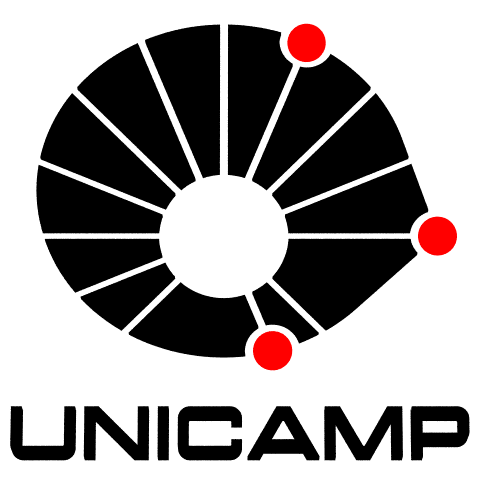
\includegraphics[width=1.5cm]{unicamp}
        \label{fig:unicamp}
    \end{subfigure}
    \hfill
    % FEEC logo
    \begin{subfigure}{0.45\textwidth}
        \centering
        
\includegraphics[width=1.5cm]{feec}
        \label{fig:feec}
    \end{subfigure}
\end{figure}

\title{EFC2 - Exercise 2}
\author{Rafael Claro Ito}
%R.A.: 118430
%ito.rafael@gmail.com
\date{September 2019}
\maketitle
\newpage

%=================================================
\section{Source files}
%=================================================

\paragraph{All code presented and all figures showed here can be found at the following GitHub repository:\\
\url{https://github.com/ito-rafael/IA006C-MachineLearning/tree/master/efc2}\\
In this repository, one can found the following files:\\}

\begin{itemize}
    \item Jupyter Notebook
    \begin{itemize}
        \item \href{https://github.com/ito-rafael/IA006C-MachineLearning/blob/master/efc2/efc2_pre-ex1.ipynb}{efc2\_pre-ex1.ipynb}
        \item \href{https://github.com/ito-rafael/IA006C-MachineLearning/blob/master/efc2/efc2_ex1_binary_classification.ipynb}{efc2\_ex1\_binary\_classification.ipynb}
        \item \href{https://github.com/ito-rafael/IA006C-MachineLearning/blob/master/efc2/efc2_ex2_multiclass_classification.ipynb}{efc2\_ex2\_multiclass\_classification.ipynb}
        \item \href{https://github.com/ito-rafael/IA006C-MachineLearning/blob/master/efc2/efc2_ex2_knn.ipynb}{efc2\_ex2\_knn.ipynb}
    \end{itemize}
    \item \LaTeX
    \begin{itemize}
        \item \href{https://github.com/ito-rafael/IA006C-MachineLearning/blob/master/efc2/LaTeX/efc2.tex}{efc2.tex}
    \end{itemize}
\end{itemize}

\paragraph{The notebook "efc2\_pre-ex1" plots the histograms for the exercise 1 and it is mainly used for data visualization. It shows the input features histograms for the raw data and also after a data stardardization.}

\paragraph{The notebook "efc2\_ex1\_binary\_classification" effectively implements the logistic regression used to perform a binary classification.}

\paragraph{The notebooks "efc2\_ex2\_multiclass\_classification" and "efc2\_ex2\_knn" implements the algorithms to perform a multiclass classification proposed in exercise 2. The former one uses the softmax approach while latter one implements the K-Nearest Neighbors (KNN) algorithm.}

%=================================================
\section{Part 1 - Binary Classification}
%=================================================

%=======================================
\subsection{a) Input features characteristics analysis considering the histograms and correlation measures between them.}
%=======================================

\paragraph{The first thing we did before starting this exercise was to plot all the data, as can be seen in figure \ref{fig:pre-ex1-logistic}.}

%\paragraph{In this method, only past data is used to predict forward-looking data. The first fold is formed by only the first year of the dataset, the year 1981, while the year used at the validation step is the next year, 1982. The second fold uses all the data of the previous fold (train plus validation) as the data to be trained, and the next year, 1983, as the validation data. Doing this for all the folds we get the configuration showed in figure \ref{fig:pre-ex1-kfold}.}

% histograms of raw features

\begin{figure}
    \centering
    % sd
    \begin{subfigure}{0.32\textwidth}
        \centering
        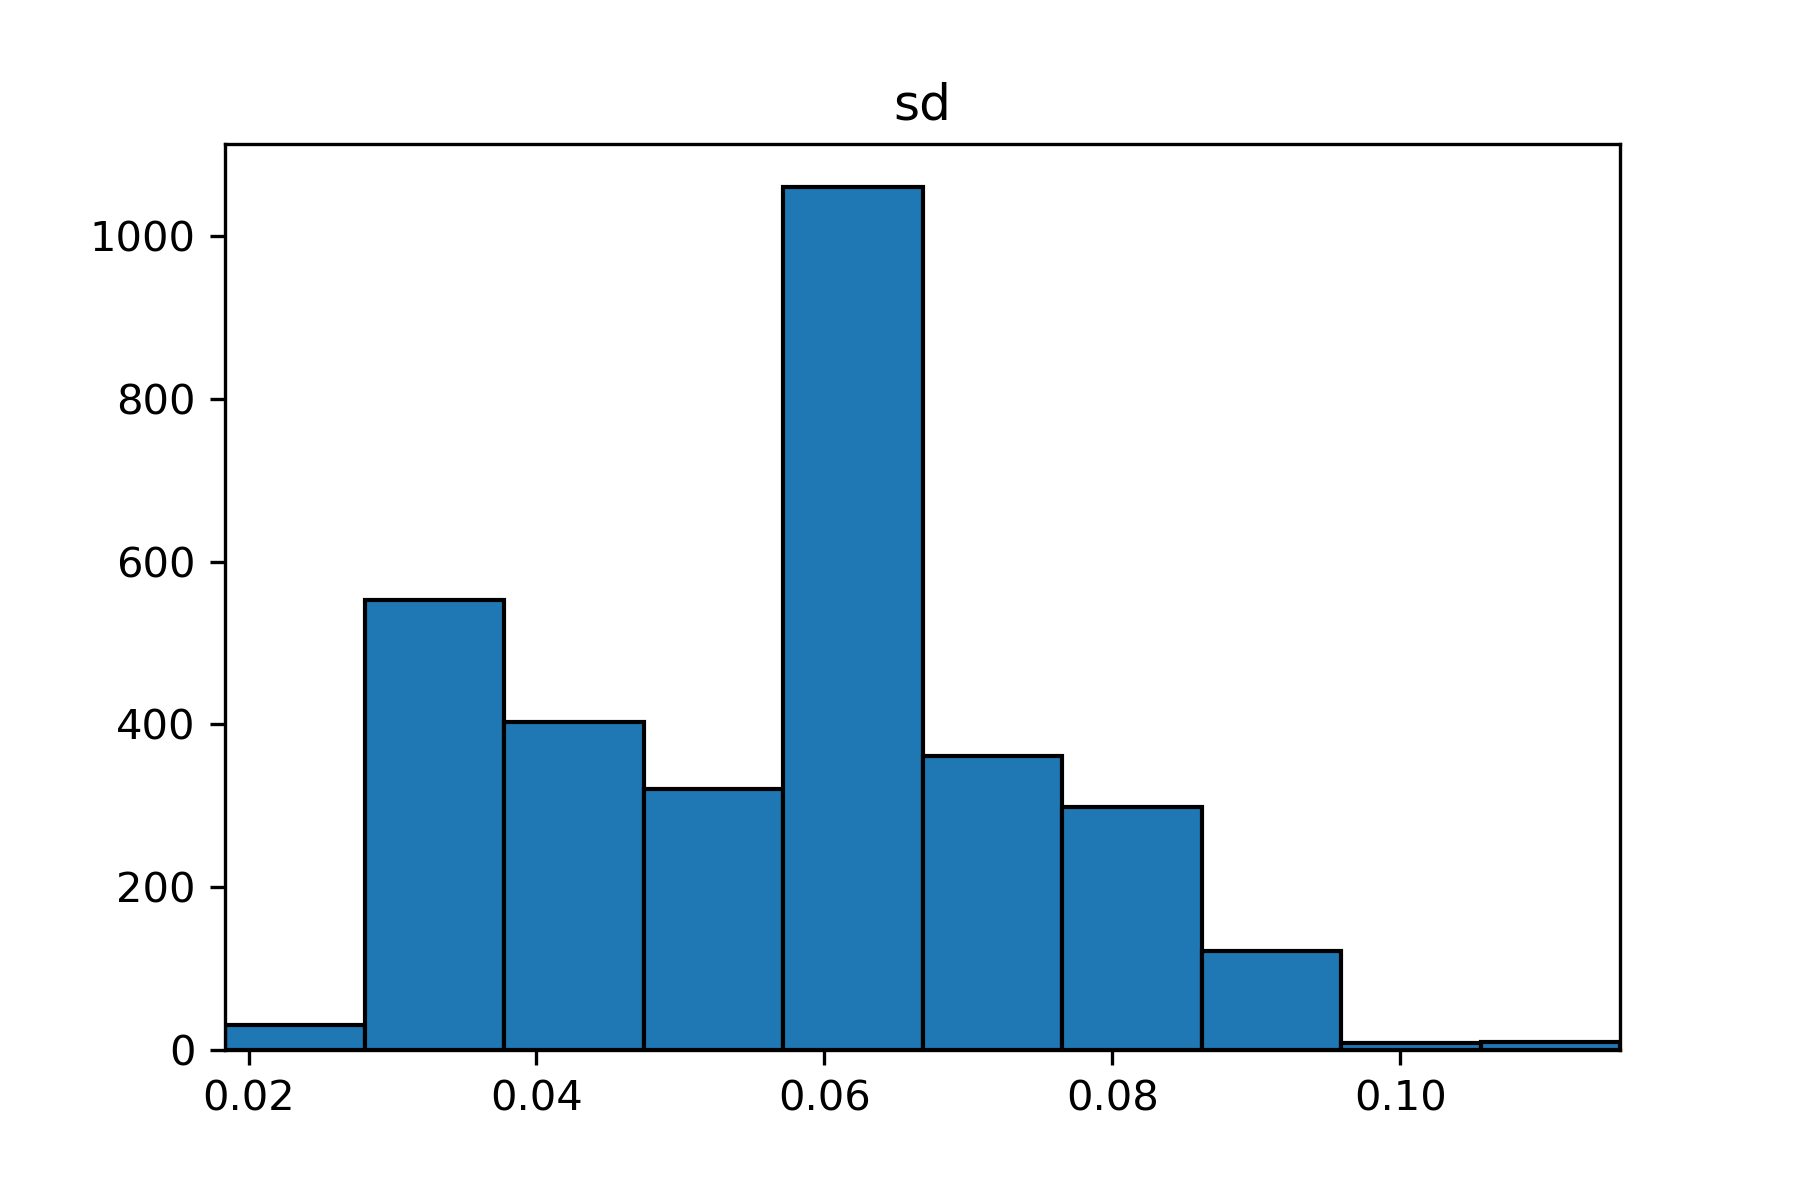
\includegraphics[width=3.85cm]{raw_0_sd}
        \caption{sd}
        \label{fig:sub_raw_1}
    \end{subfigure}
    \hfill
    % median
    \begin{subfigure}{0.32\textwidth}
        \centering
        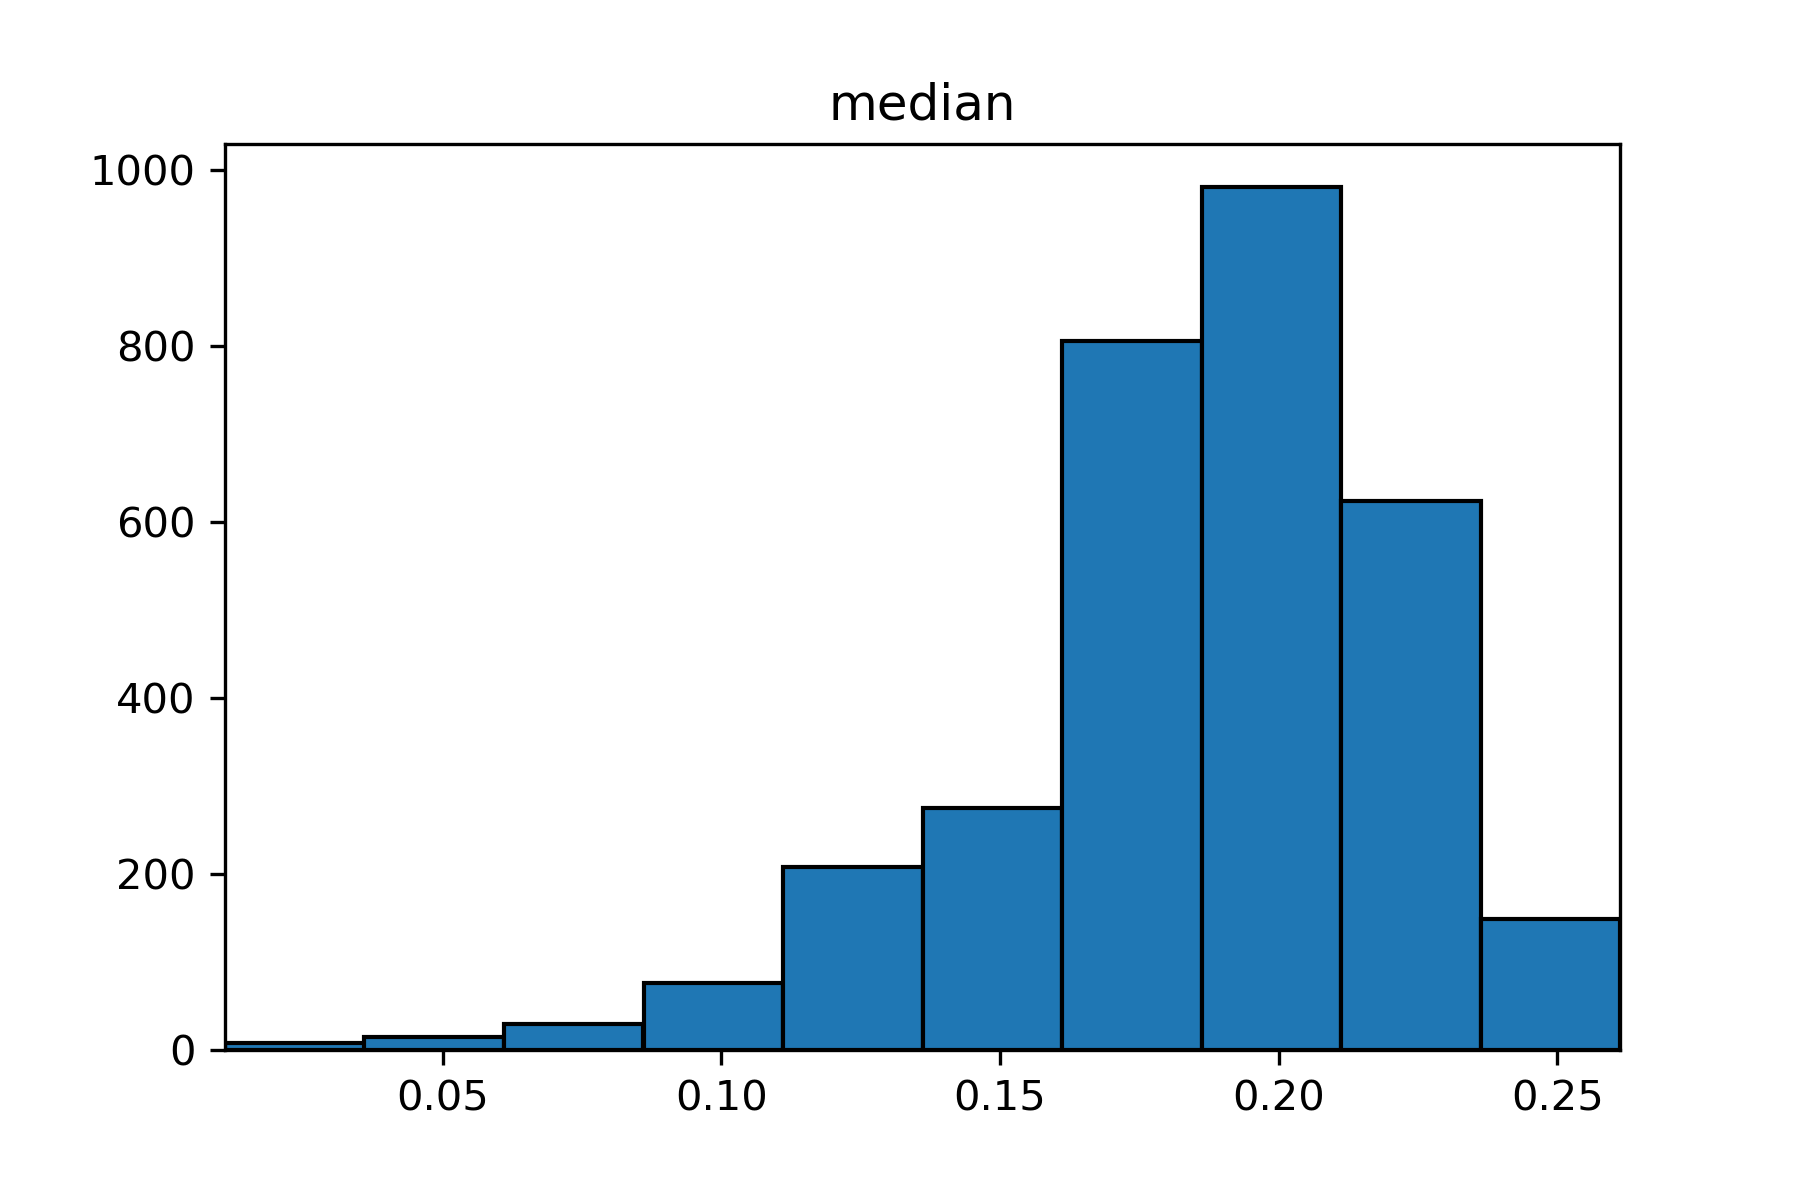
\includegraphics[width=3.85cm]{raw_1_median}
        \caption{median}
        \label{fig:sub_raw_2}
    \end{subfigure}
    \hfill
    % Q25
    \begin{subfigure}{0.32\textwidth}
        \centering
        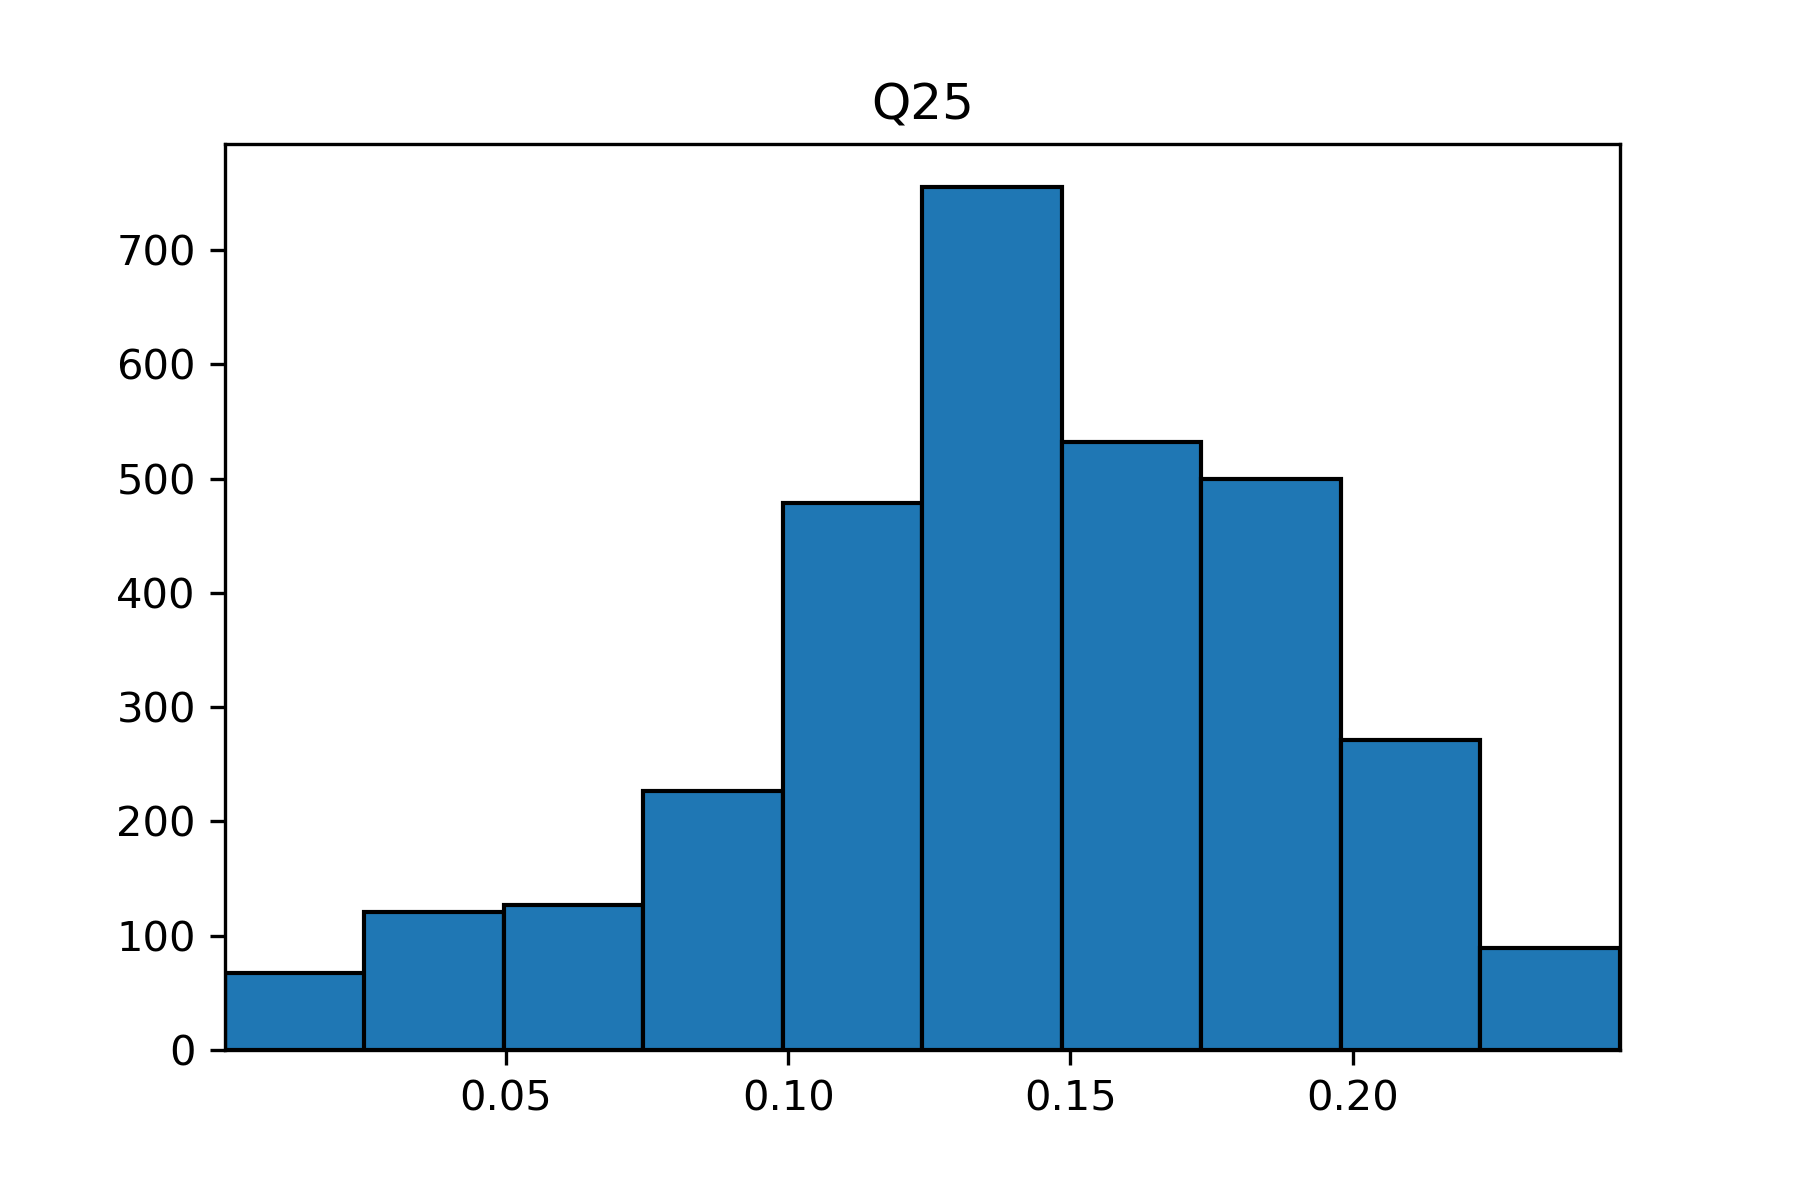
\includegraphics[width=3.85cm]{raw_2_Q25}
        \caption{Q25}
        \label{fig:sub_raw_3}
    \end{subfigure}%
    \\
    % Q75
    \begin{subfigure}{0.32\textwidth}
        \centering
        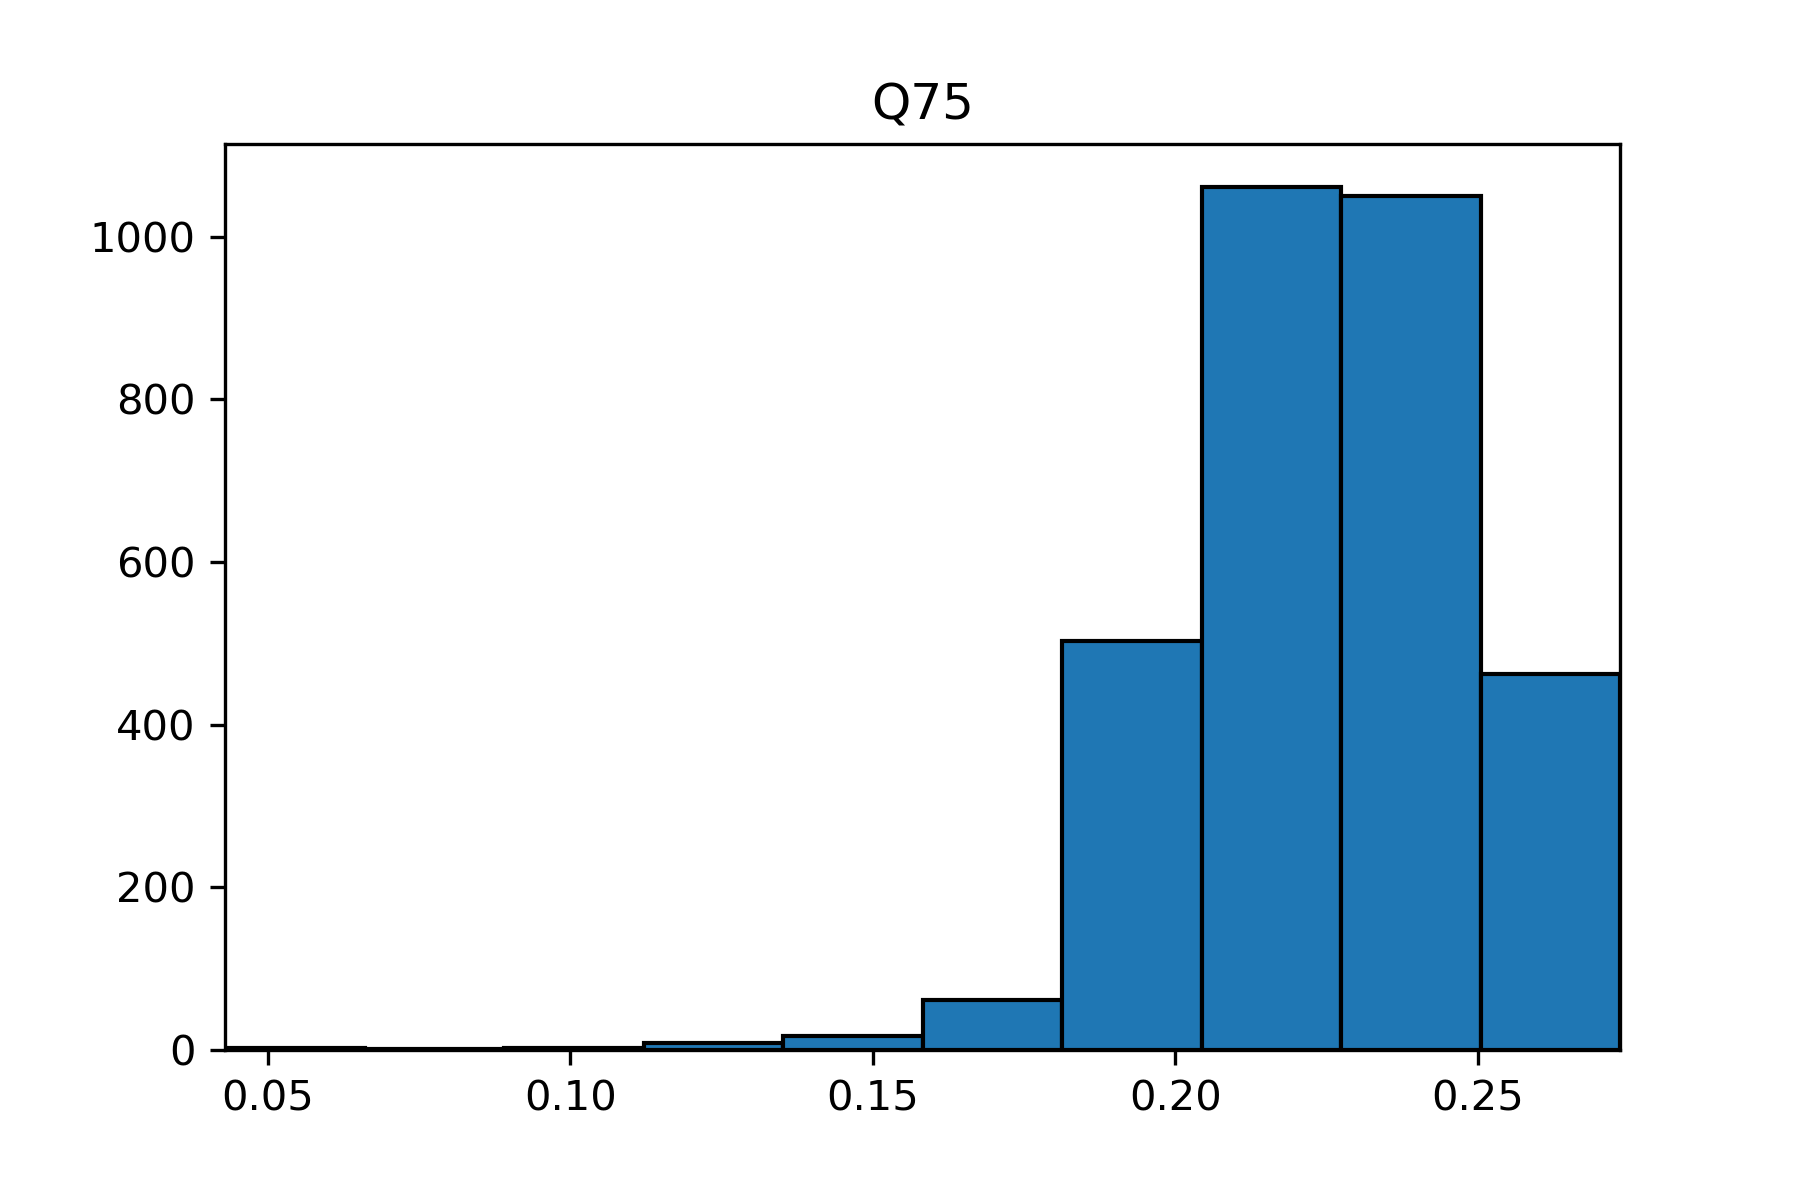
\includegraphics[width=3.85cm]{raw_3_Q75}
        \caption{Q75}
        \label{fig:sub_raw_4}
    \end{subfigure}\hfill
    % Q75
    \begin{subfigure}{0.32\textwidth}
        \centering
        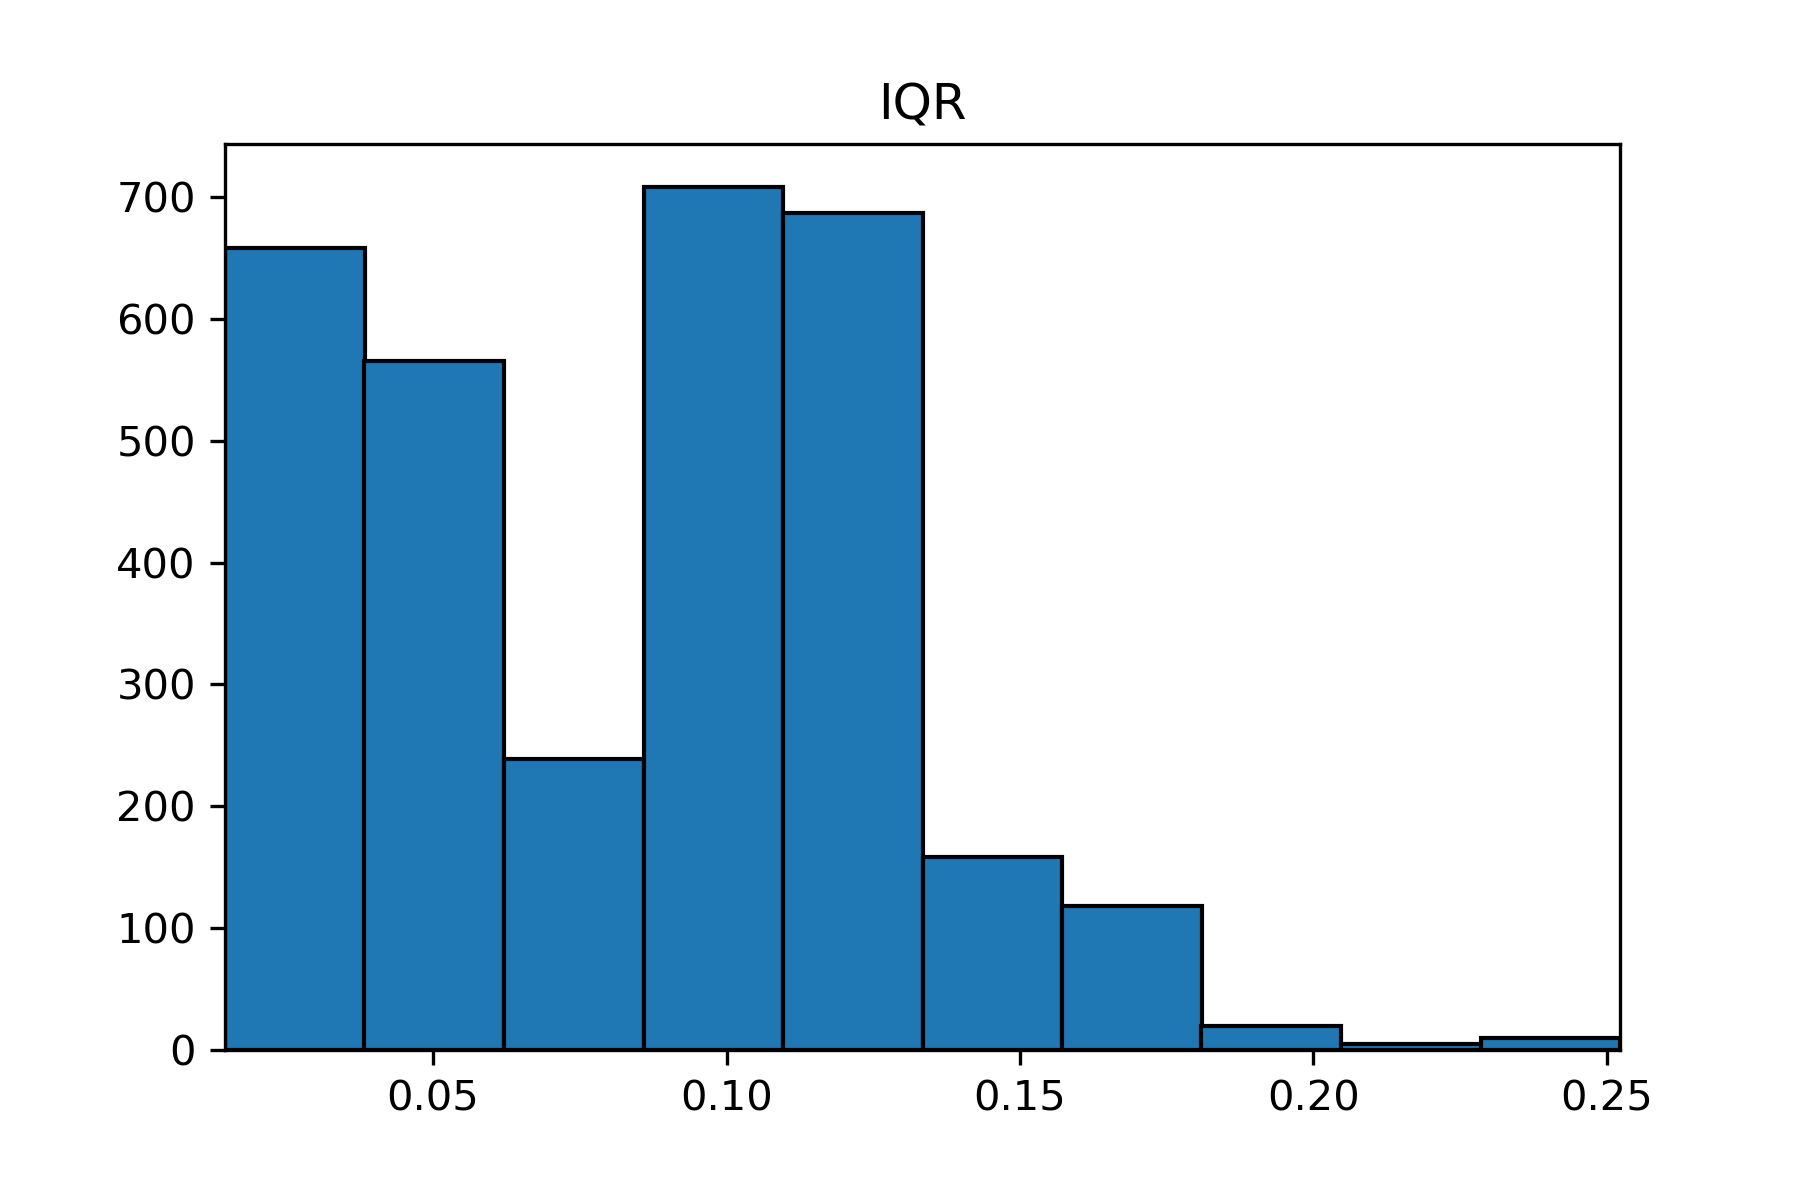
\includegraphics[width=3.85cm]{raw_4_IQR}
        \caption{IQR}
        \label{fig:sub_raw_5}
    \end{subfigure}\hfill
    % skew
    \begin{subfigure}{0.32\textwidth}
        \centering
        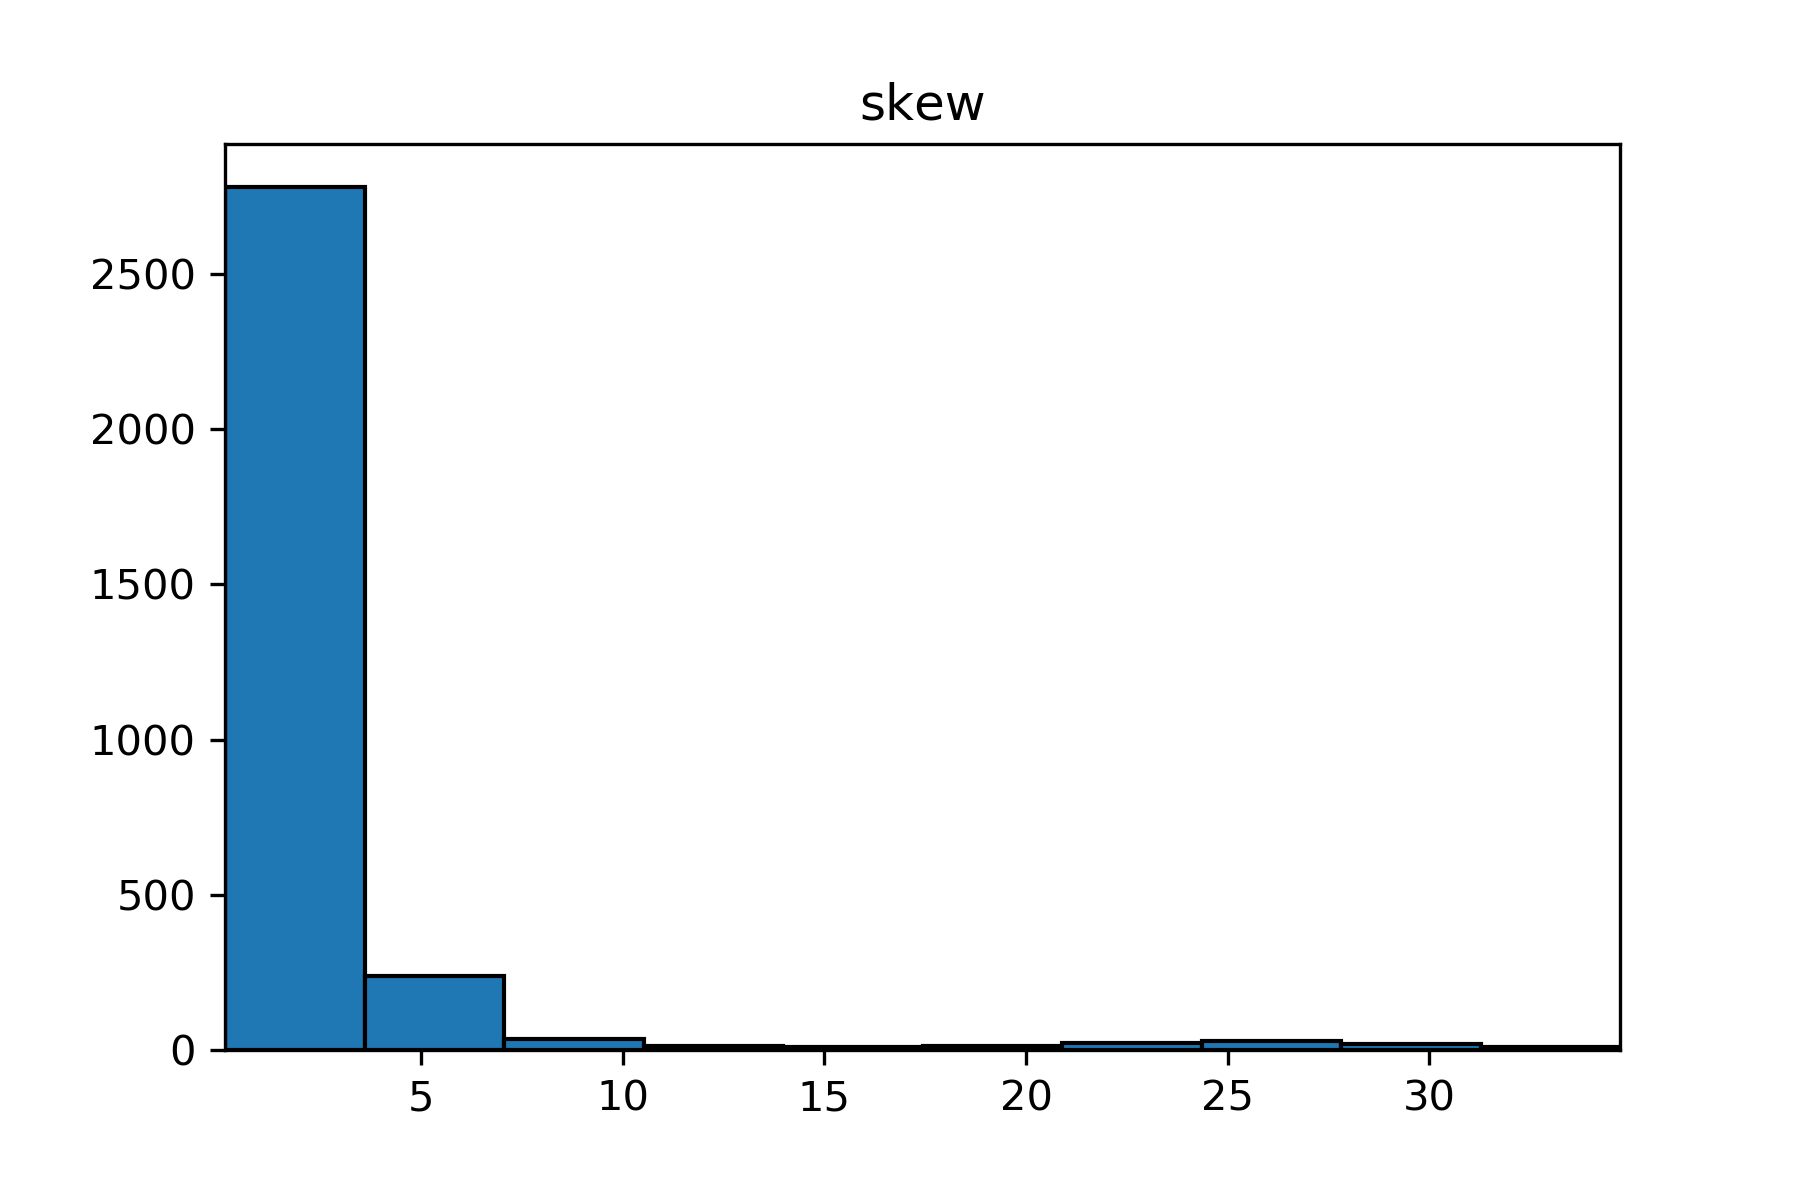
\includegraphics[width=3.85cm]{raw_5_skew}
        \caption{skew}
        \label{fig:sub_raw_6}
    \end{subfigure}
    \\
    % kurt
    \begin{subfigure}{0.32\textwidth}
        \centering
        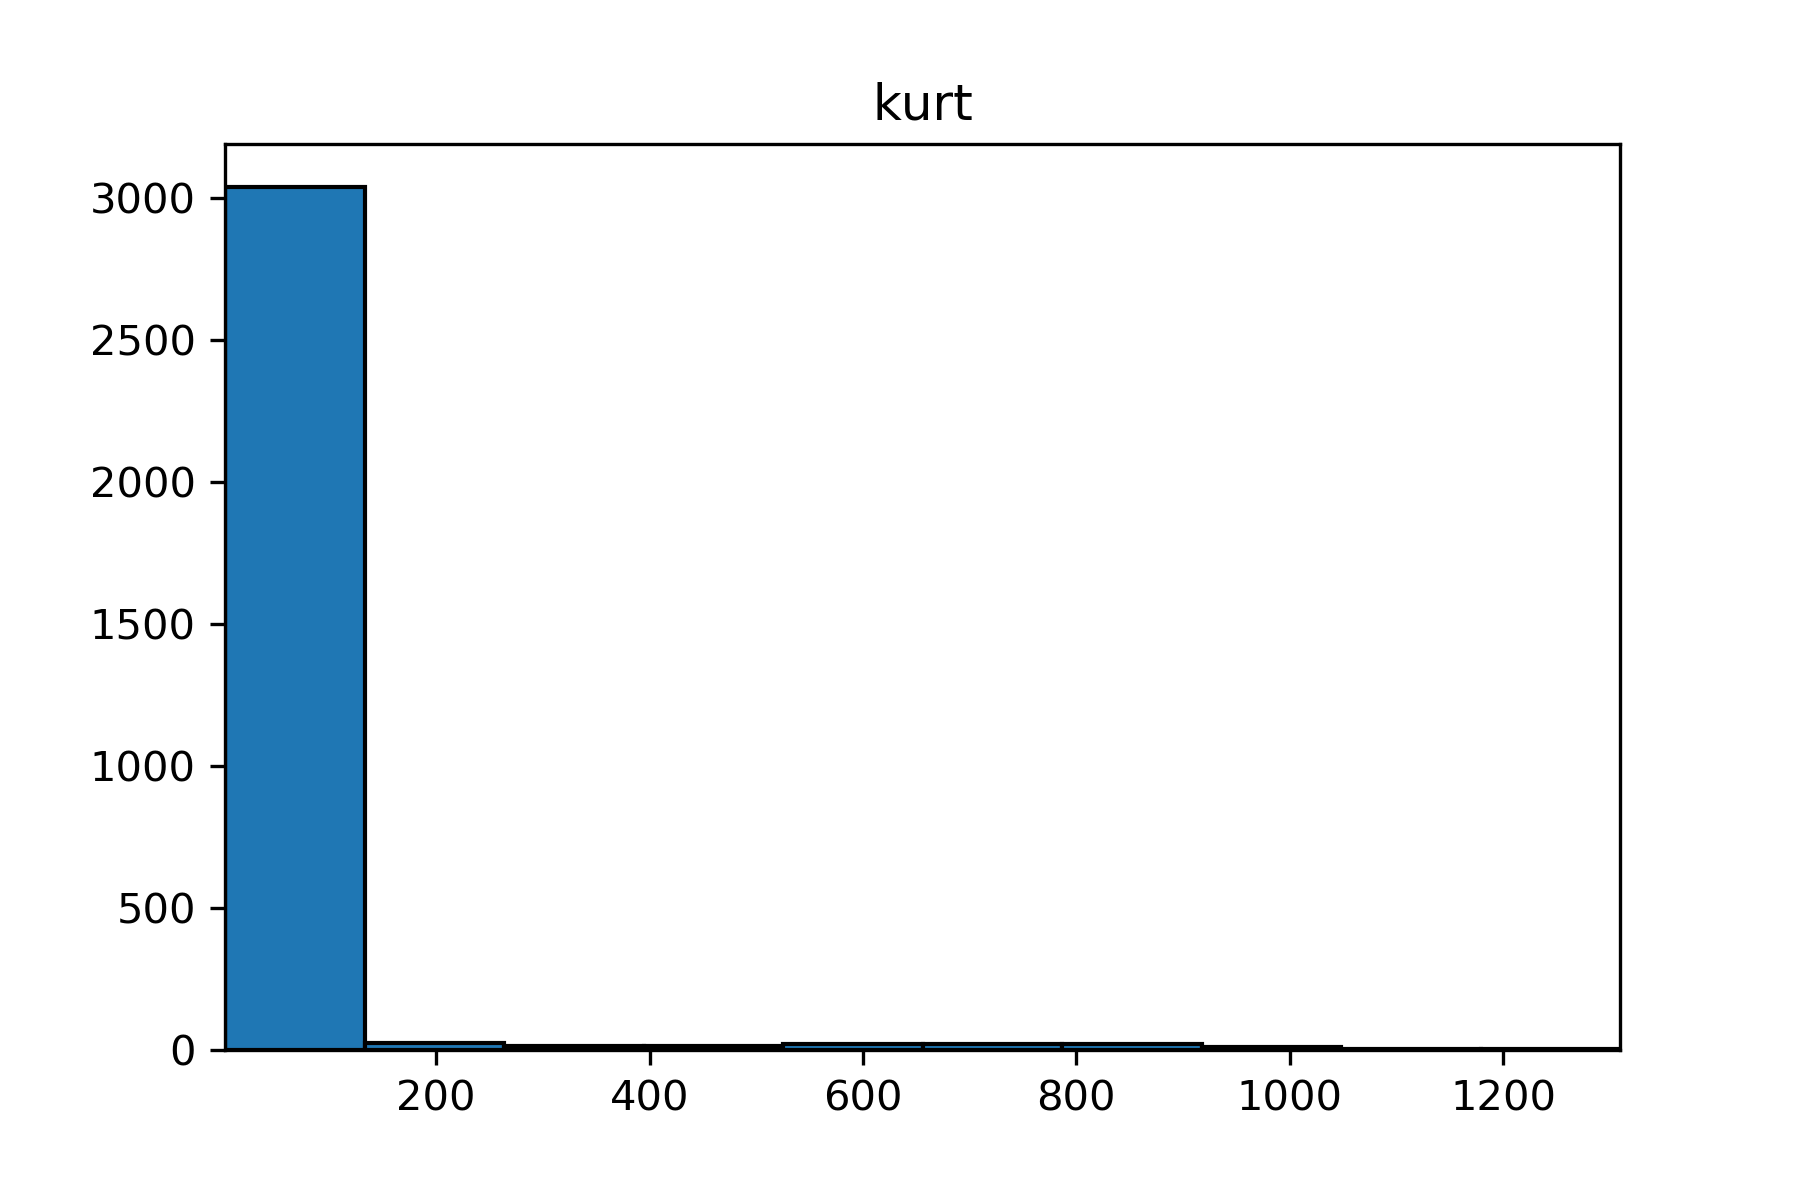
\includegraphics[width=3.85cm]{raw_6_kurt}
        \caption{kurt}
        \label{fig:sub_raw_7}
    \end{subfigure}\hfill
    % sp ent
    \begin{subfigure}{0.32\textwidth}
        \centering
        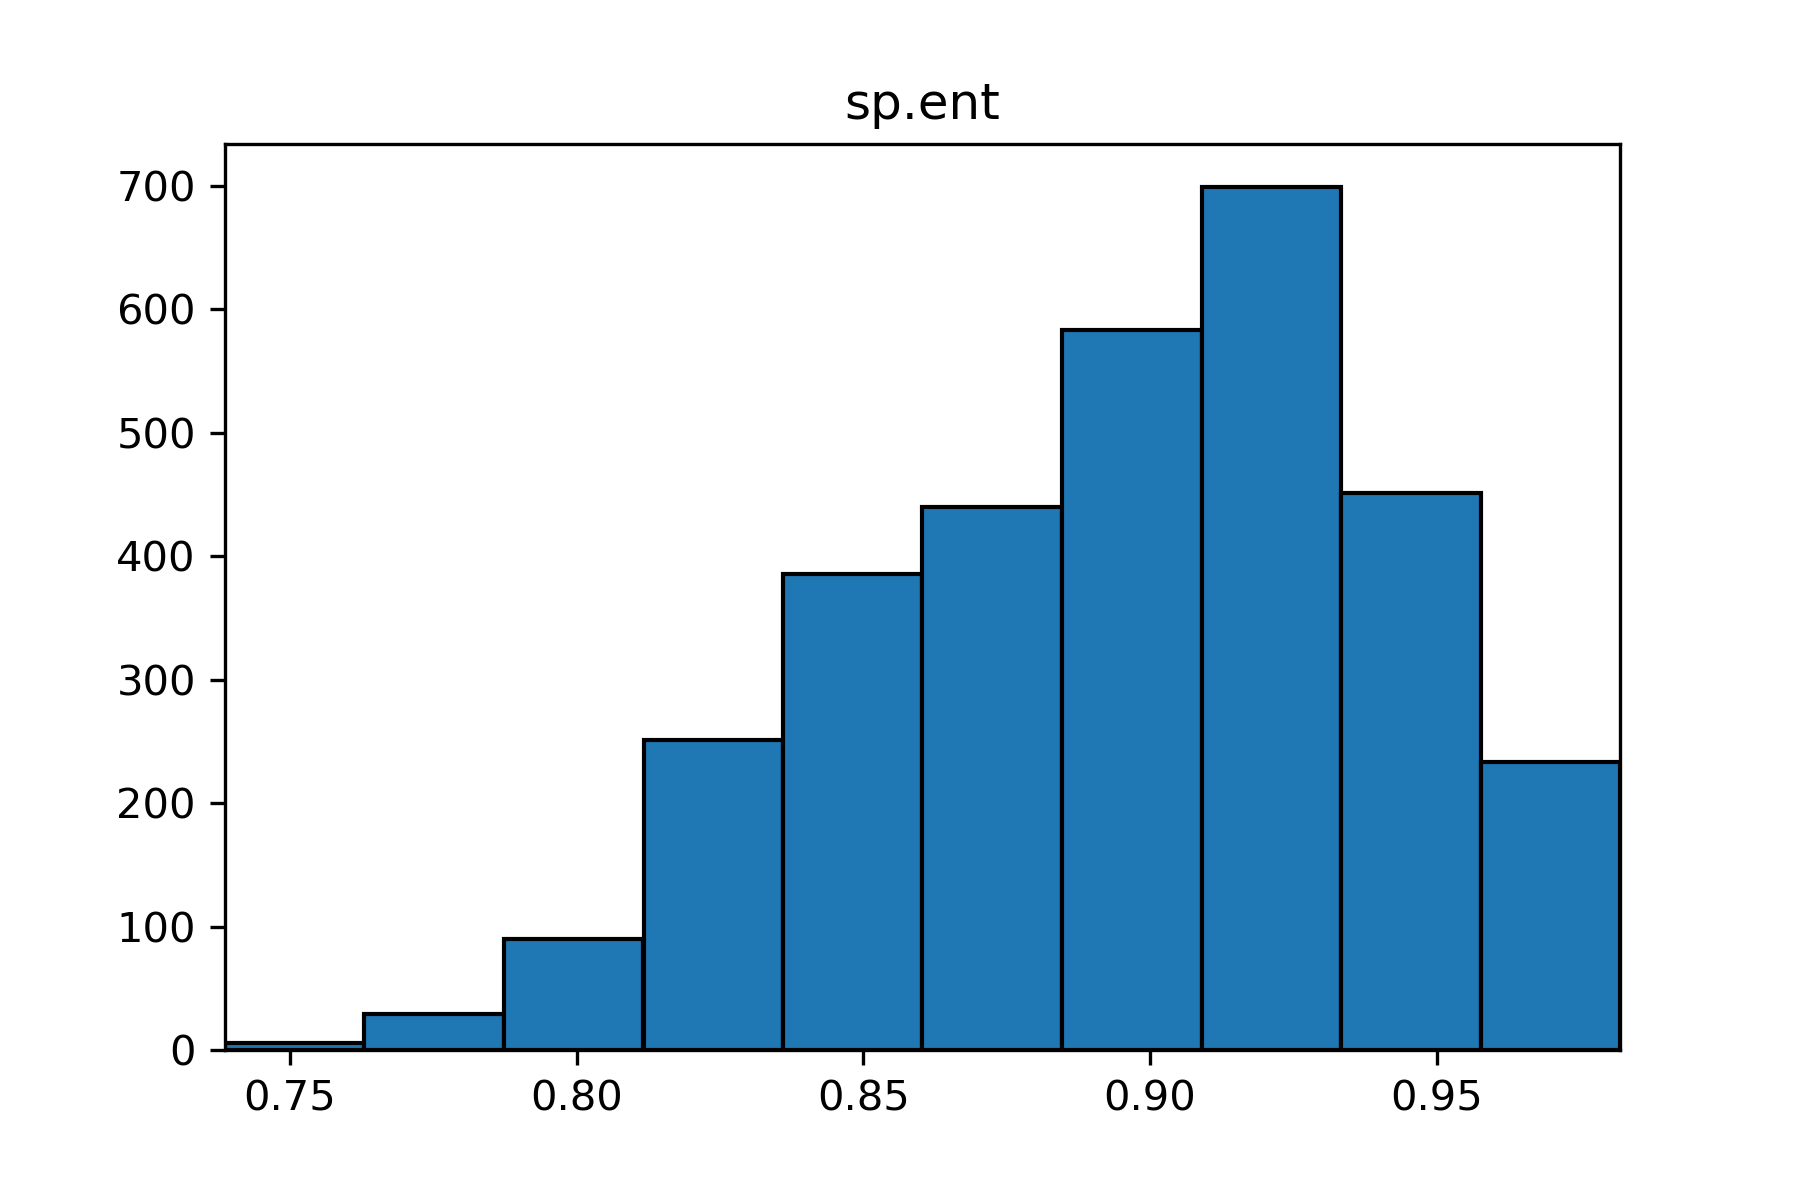
\includegraphics[width=3.85cm]{raw_7_sp_ent}
        \caption{sp ent}
        \label{fig:sub_raw_8}
    \end{subfigure}\hfill
    % sfm
    \begin{subfigure}{0.32\textwidth}
        \centering
        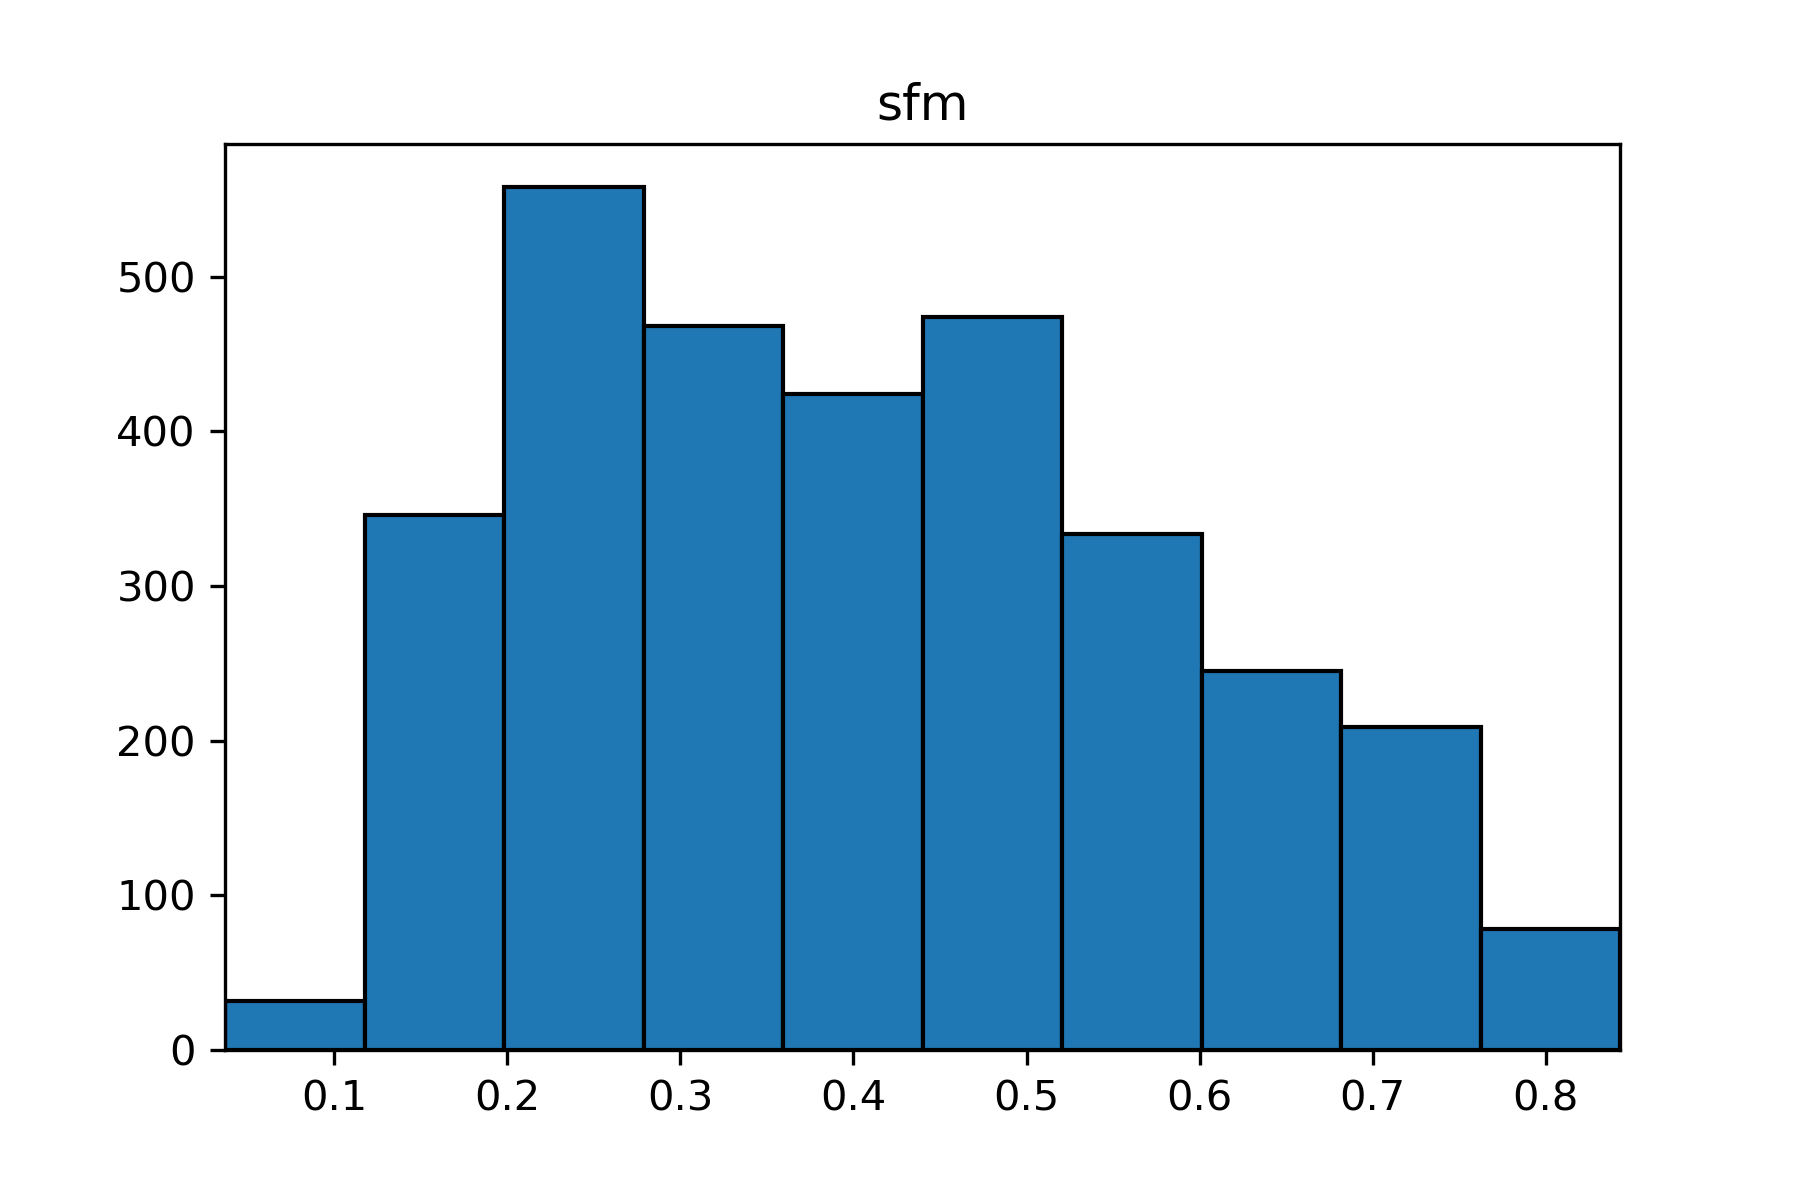
\includegraphics[width=3.85cm]{raw_8_sfm}
        \caption{smf}
        \label{fig:sub_raw_9}
    \end{subfigure}\hfill
    % mode
    \begin{subfigure}{0.32\textwidth}
        \centering
        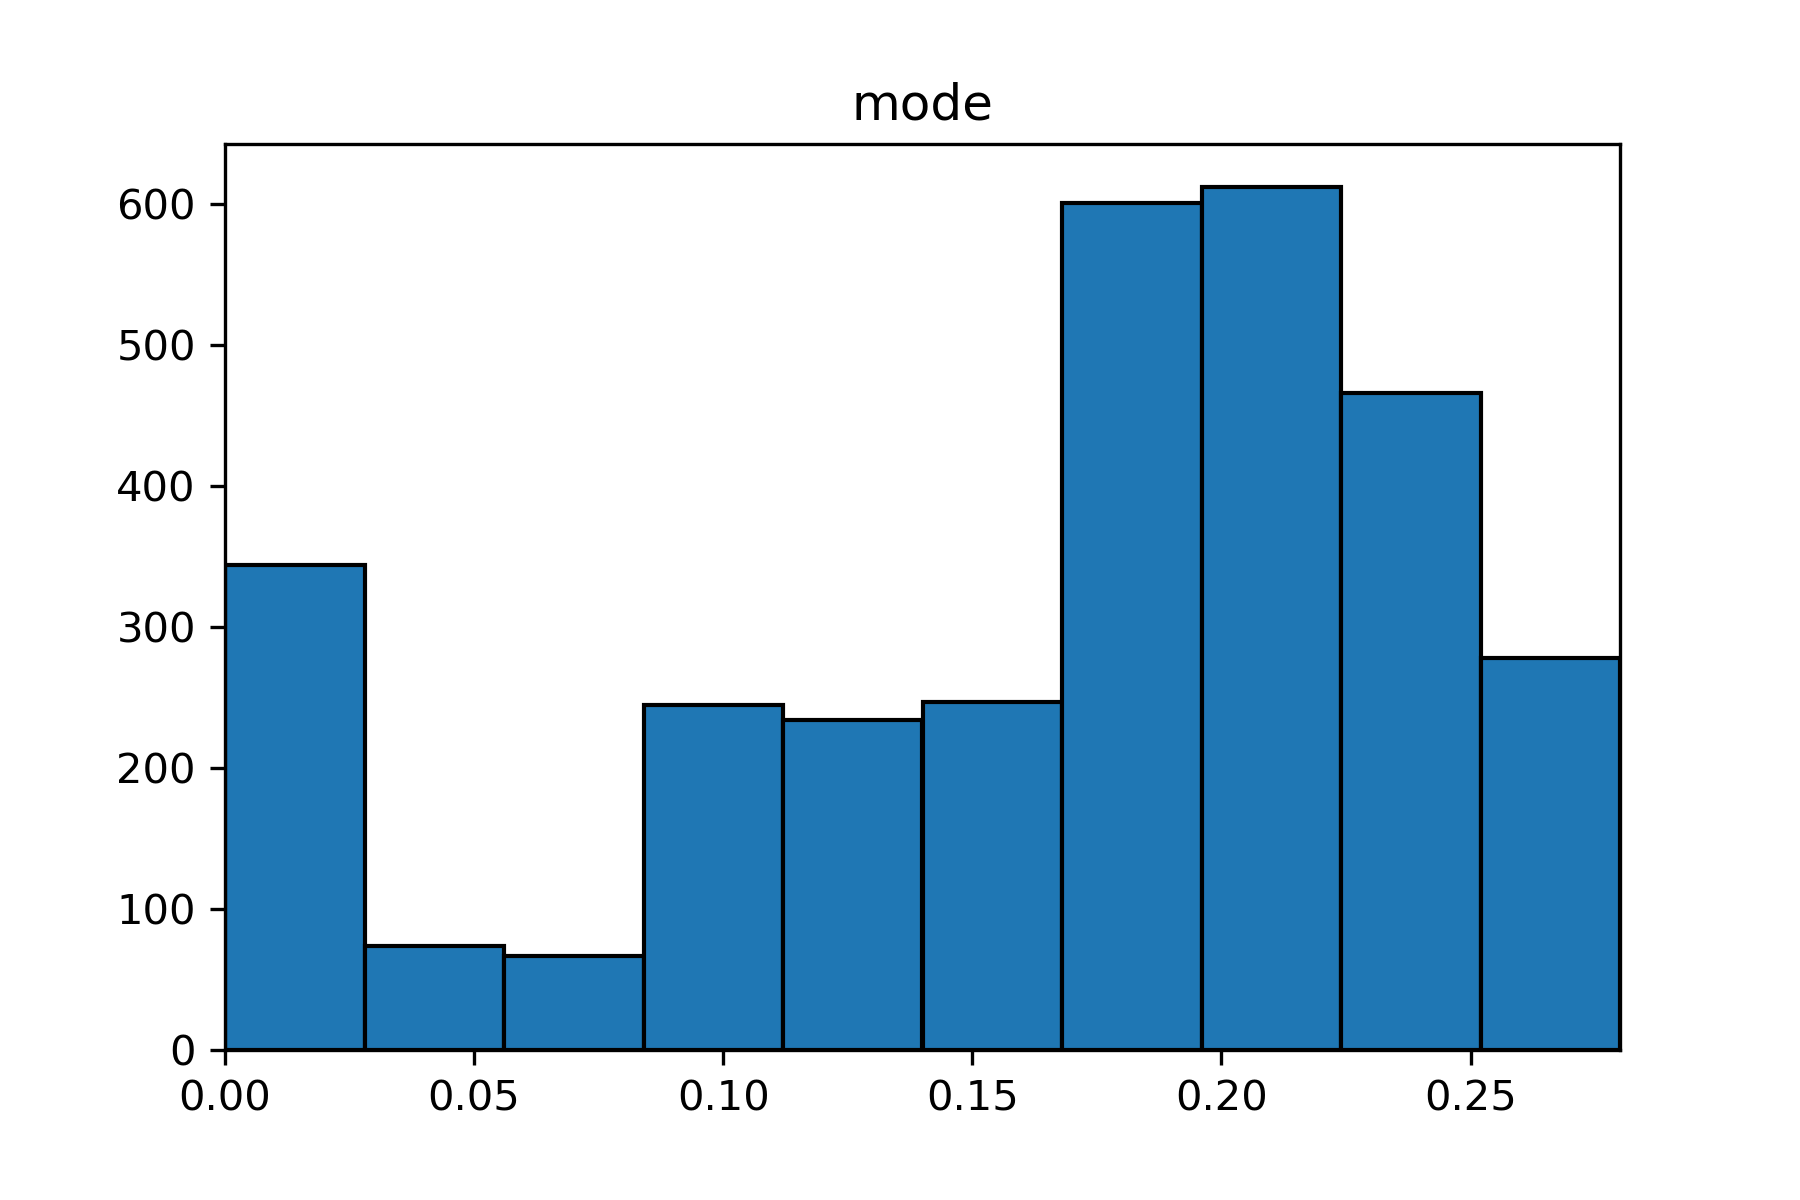
\includegraphics[width=3.85cm]{raw_9_mode}
        \caption{mode}
        \label{fig:sub_raw_10}
    \end{subfigure}\hfill
    % centroid
    \begin{subfigure}{0.32\textwidth}
        \centering
        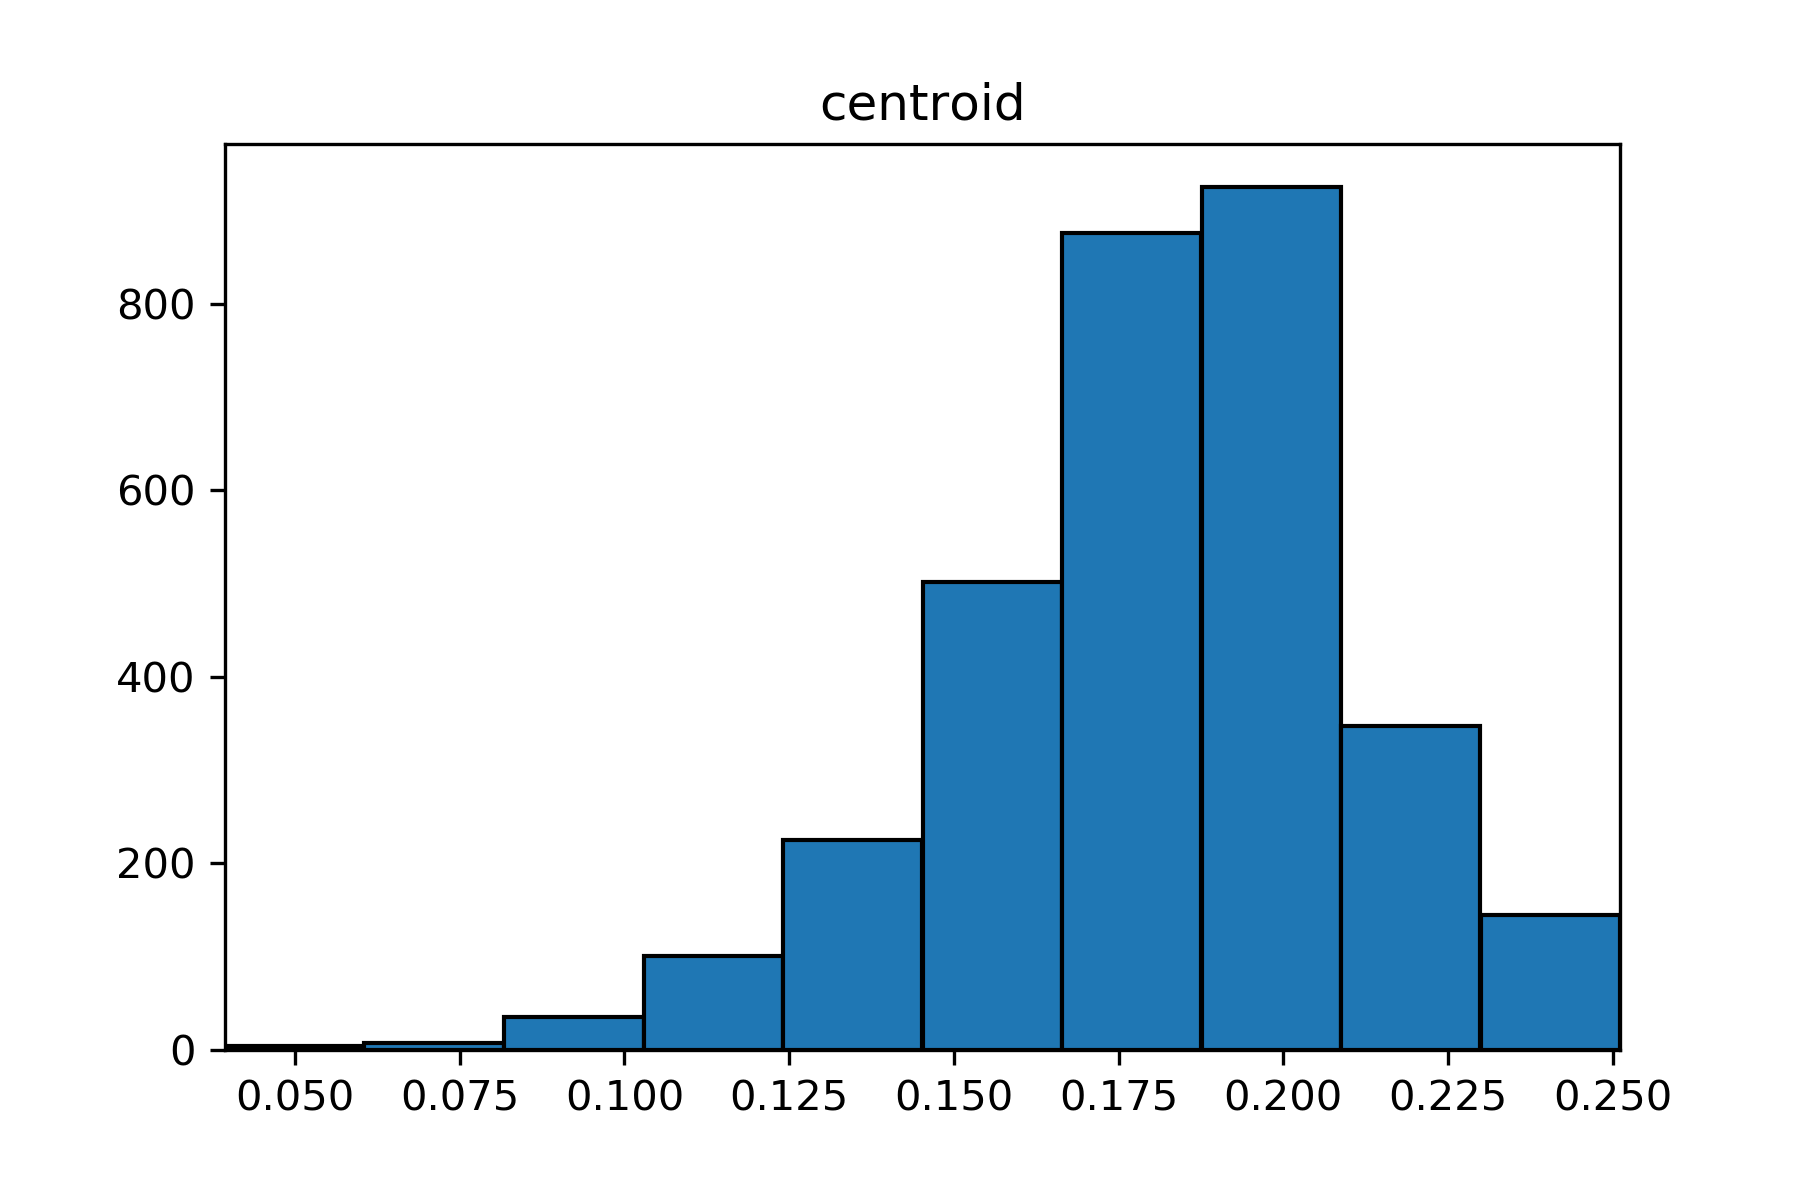
\includegraphics[width=3.85cm]{raw_10_centroid}
        \caption{centroid}
        \label{fig:sub_raw_11}
    \end{subfigure}\hfill
    % meanfun
    \begin{subfigure}{0.32\textwidth}
        \centering
        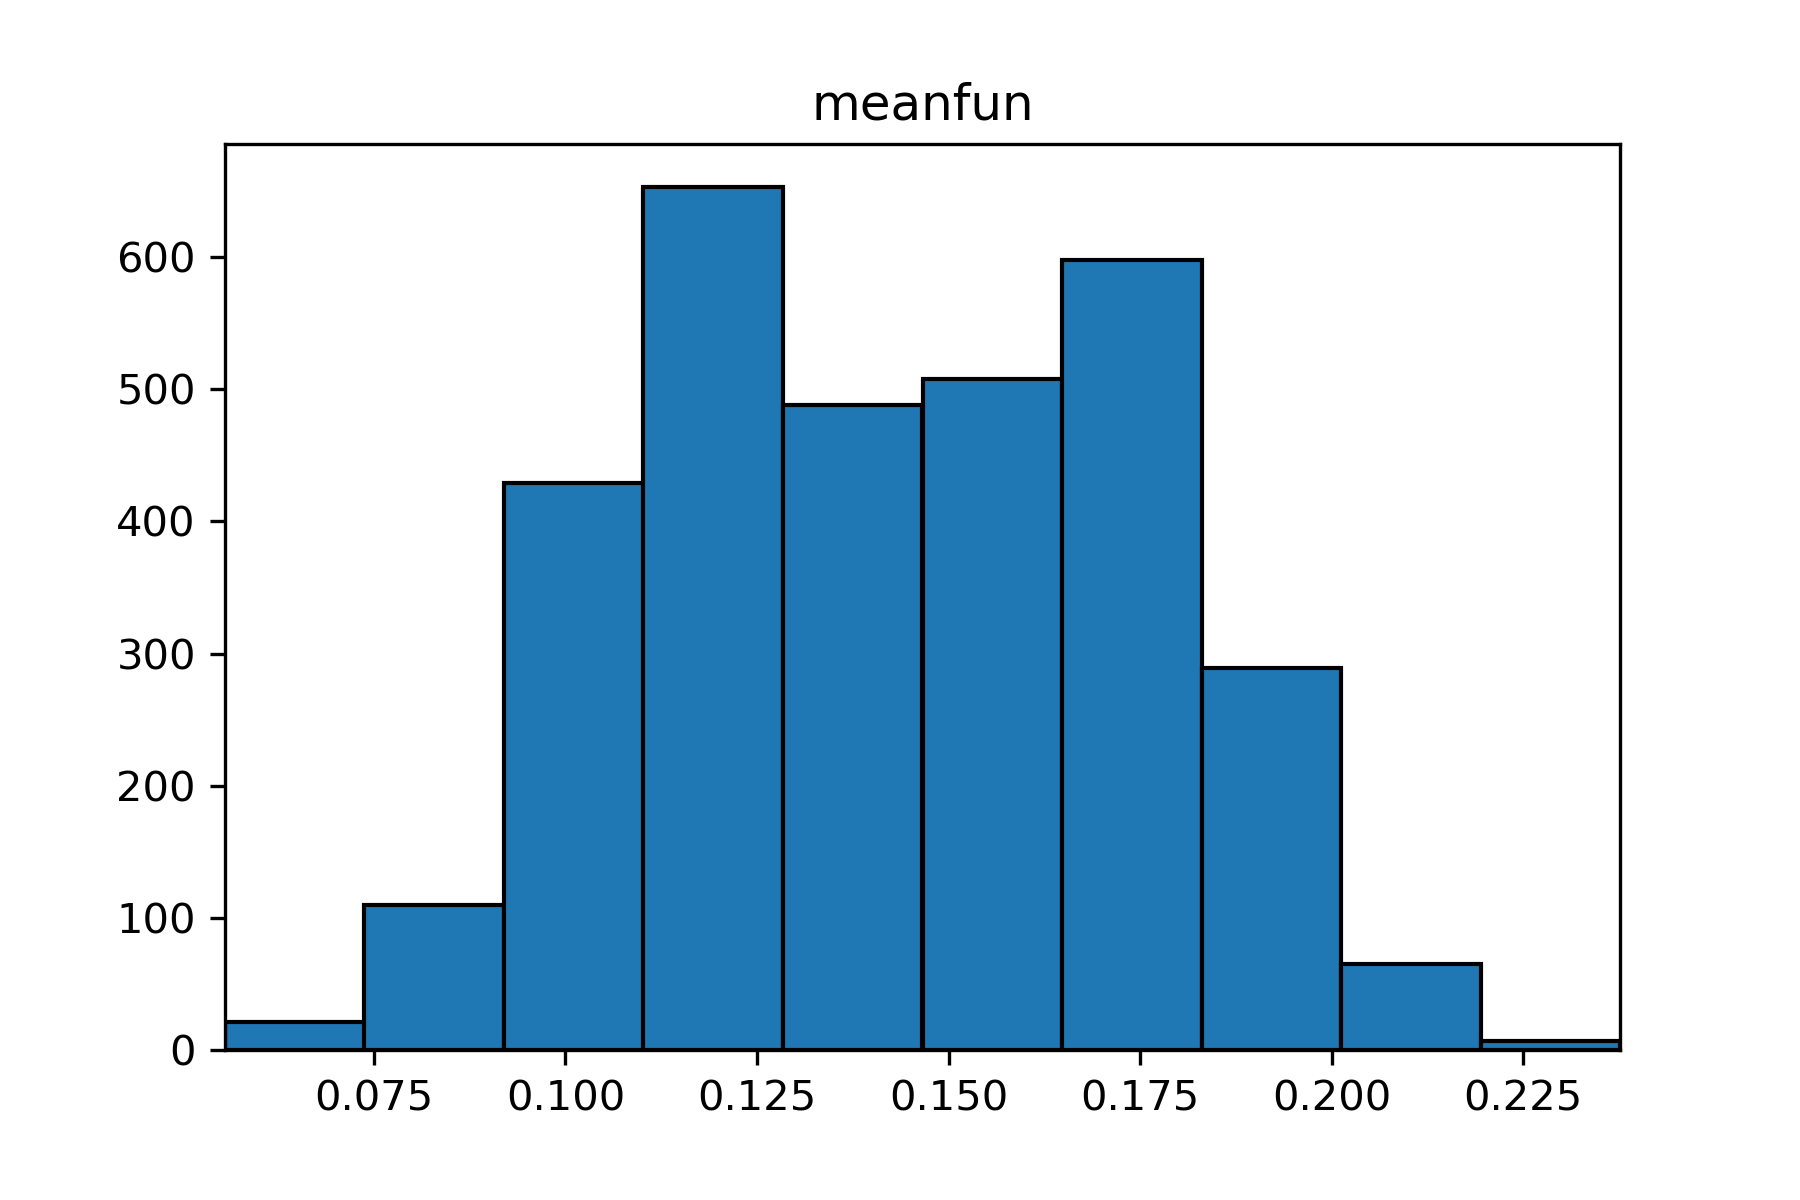
\includegraphics[width=3.85cm]{raw_11_meanfun}
        \caption{meanfun}
        \label{fig:sub_raw_12}
    \end{subfigure}\hfill
    % minfun
    \begin{subfigure}{0.32\textwidth}
        \centering
        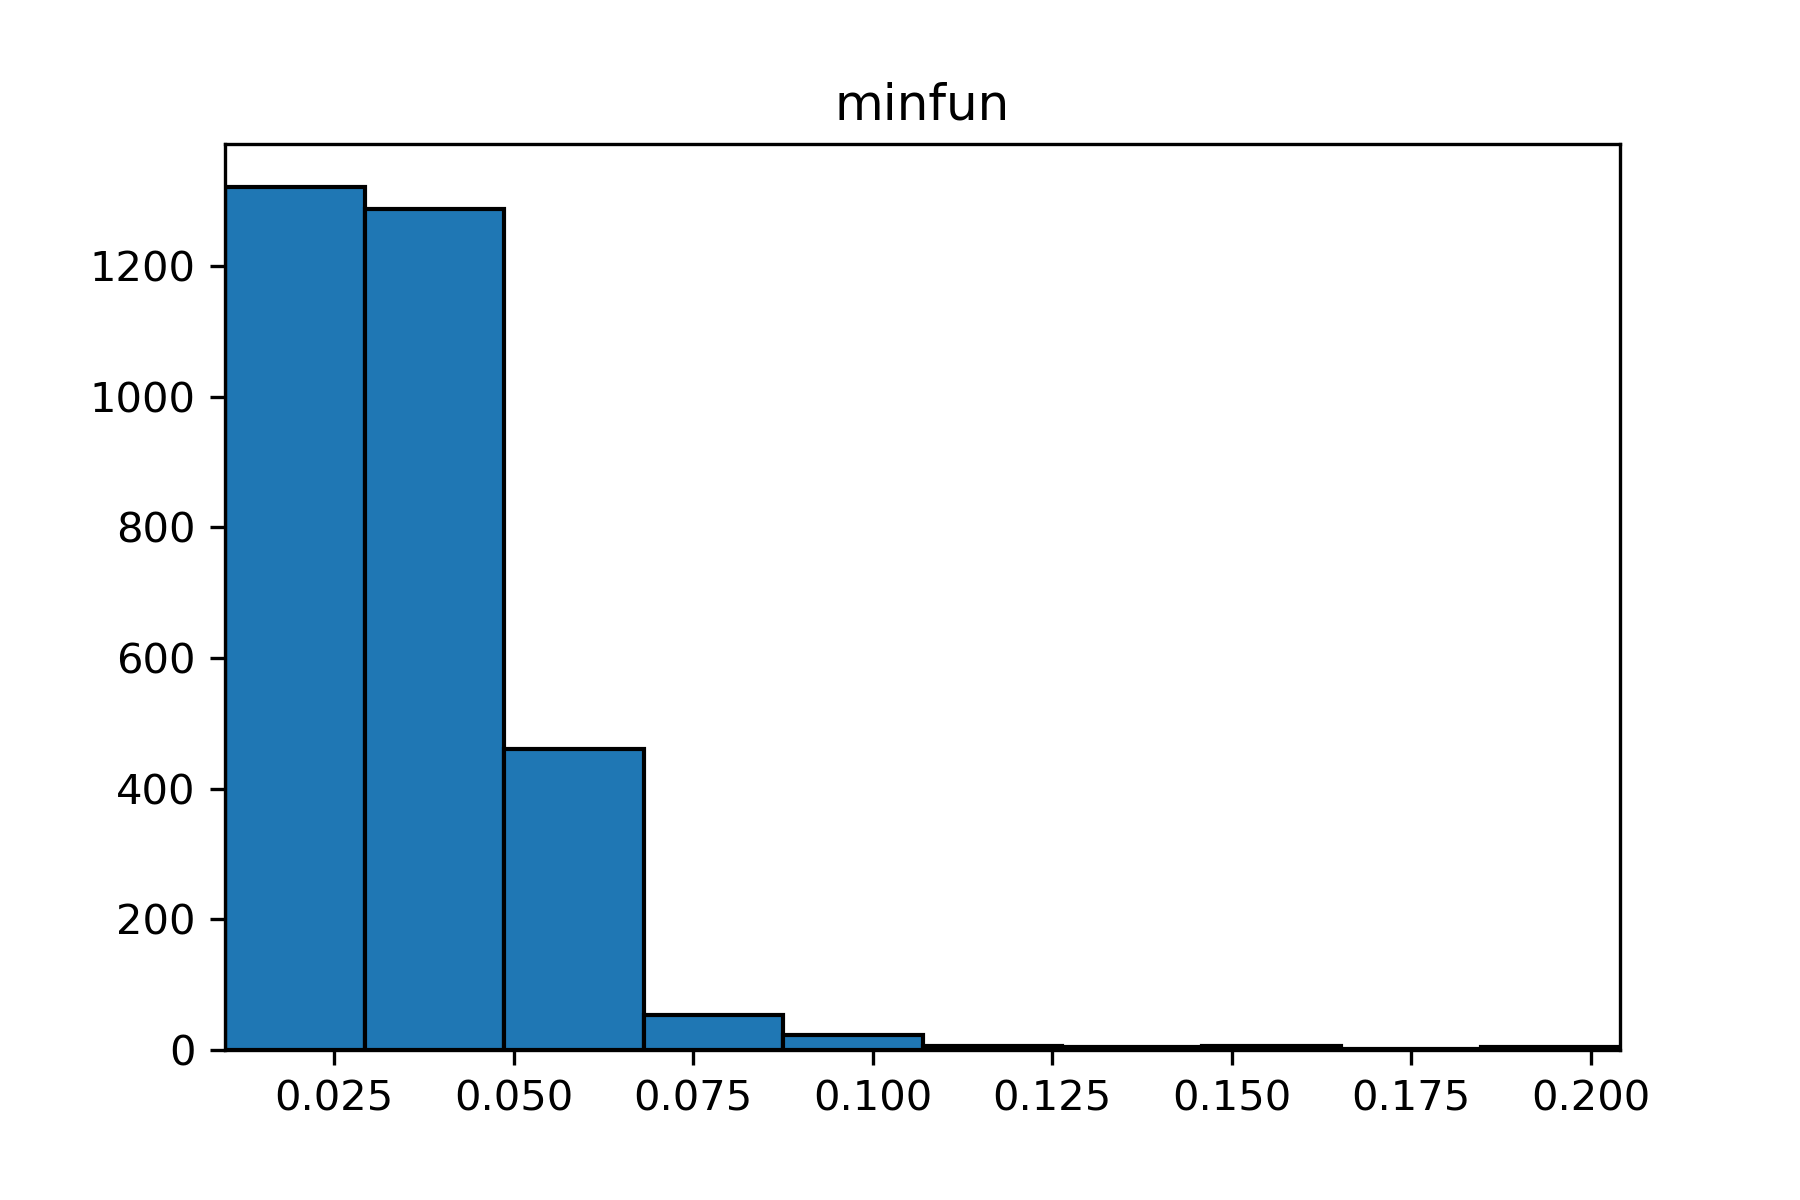
\includegraphics[width=3.85cm]{raw_12_minfun}
        \caption{minfun}
        \label{fig:sub_raw_13}
    \end{subfigure}\hfill
    % maxfun
    \begin{subfigure}{0.32\textwidth}
        \centering
        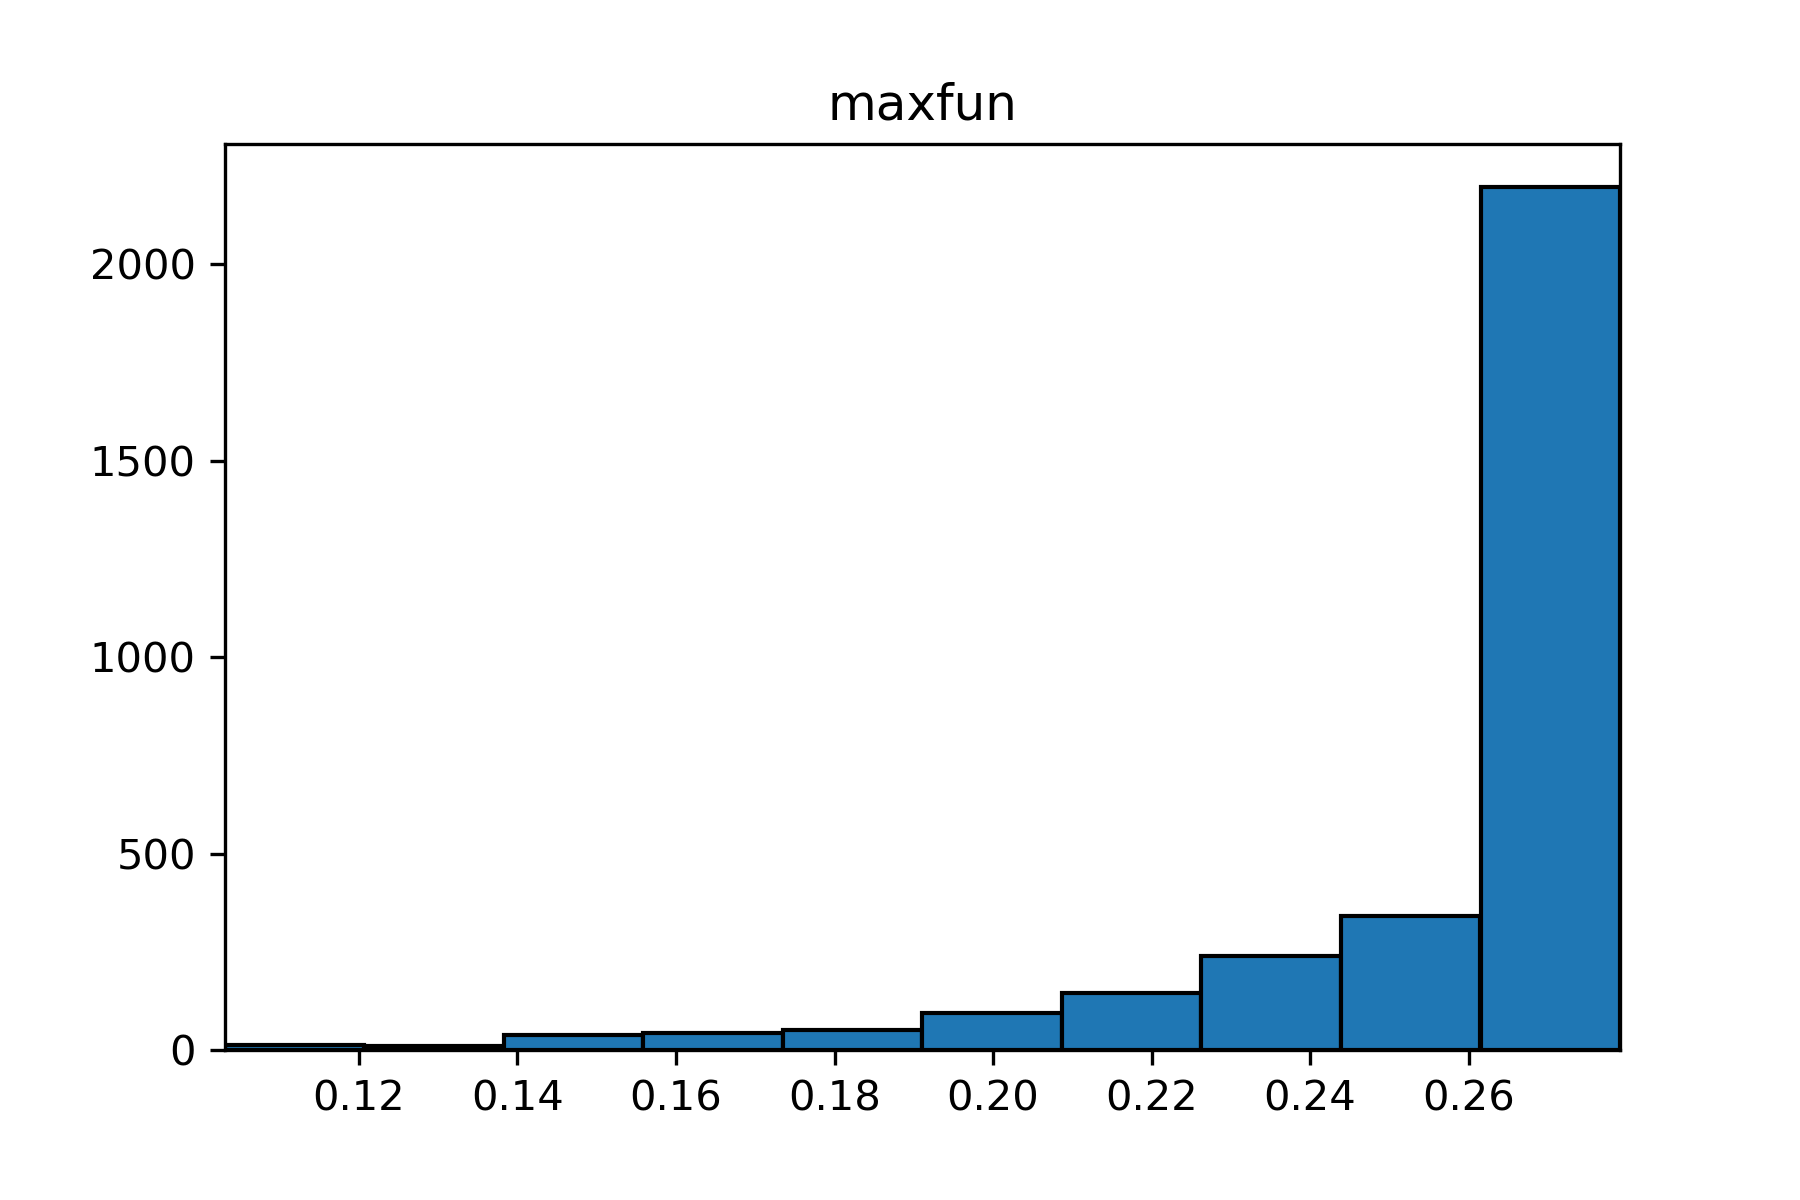
\includegraphics[width=3.85cm]{raw_13_maxfun}
        \caption{maxfun}
        \label{fig:sub_raw_14}
    \end{subfigure}\hfill
    % meandom
    \begin{subfigure}{0.32\textwidth}
        \centering
        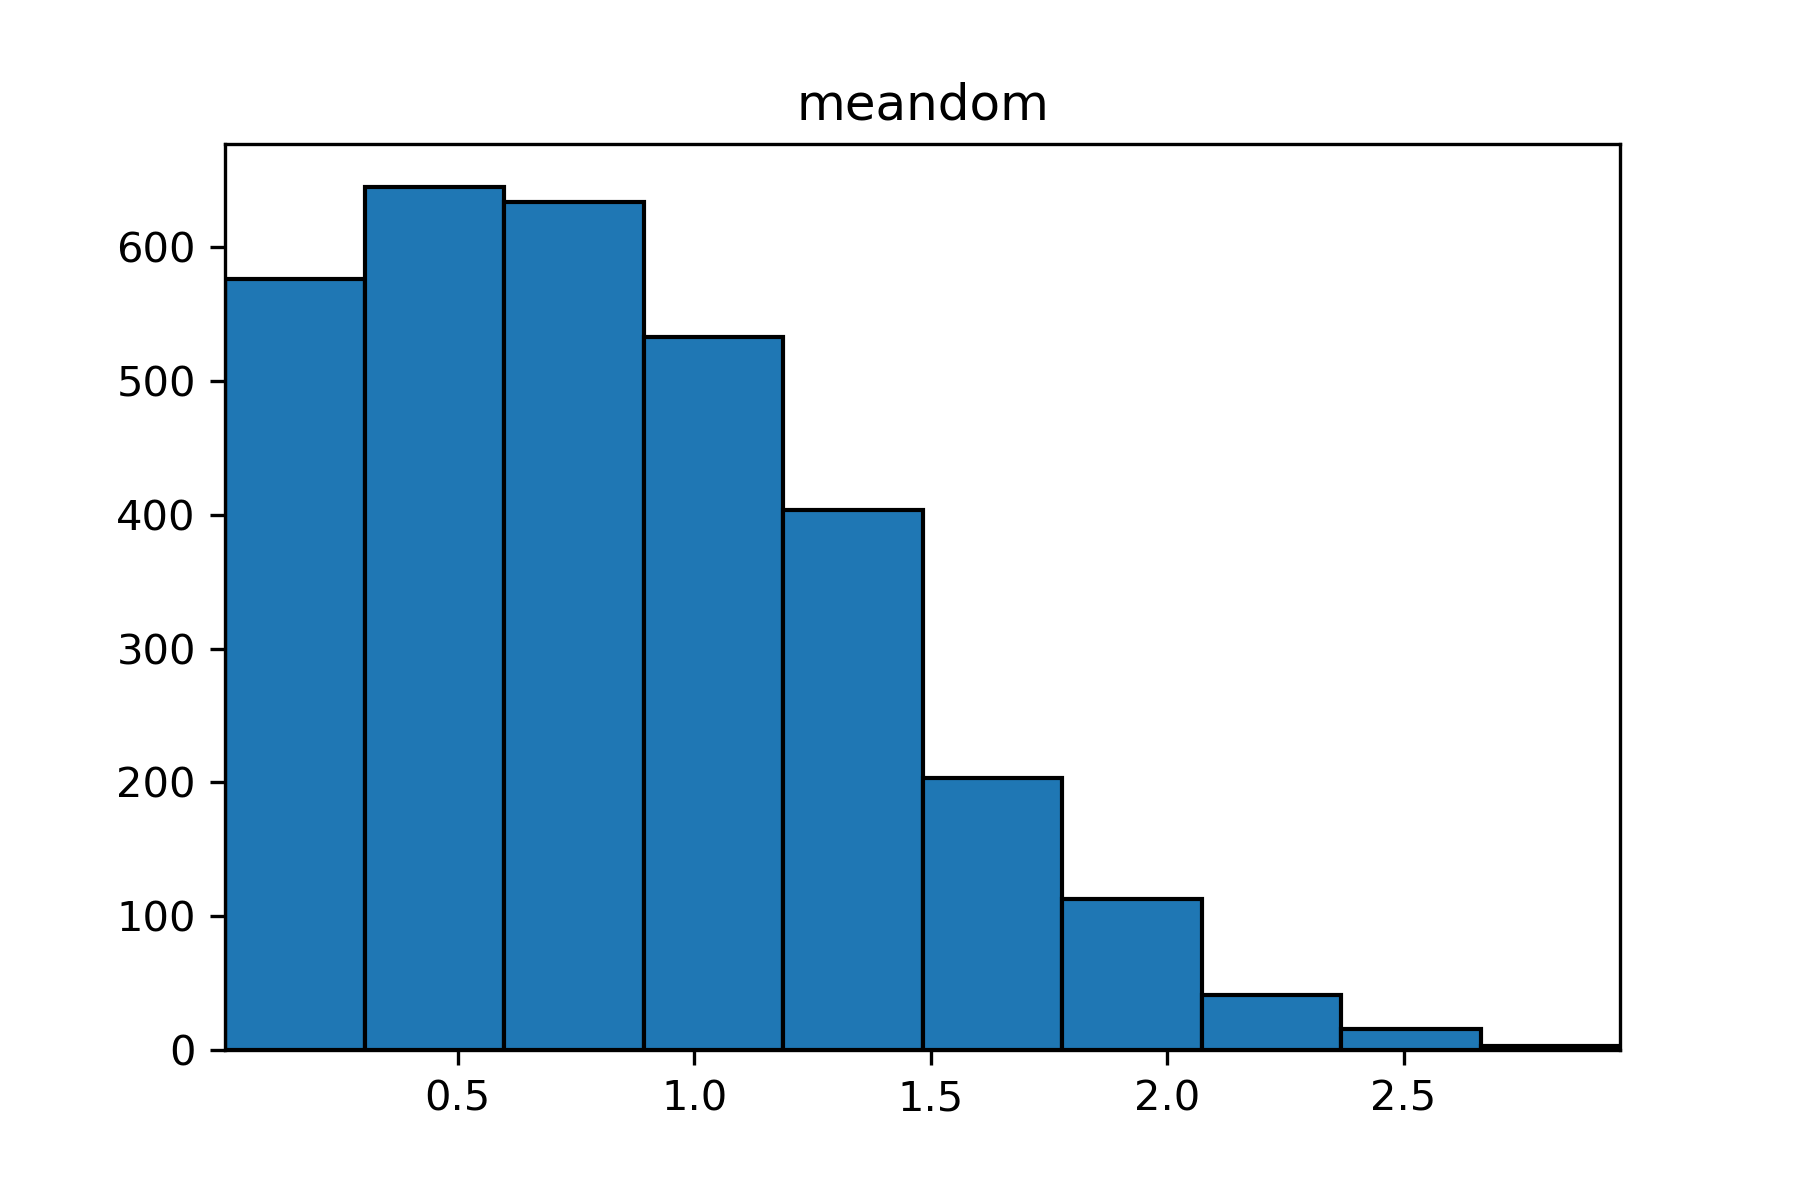
\includegraphics[width=3.85cm]{raw_14_meandom}
        \caption{meandom}
        \label{fig:sub_raw_15}
    \end{subfigure}\hfill
    % mindom
    \begin{subfigure}{0.32\textwidth}
        \centering
        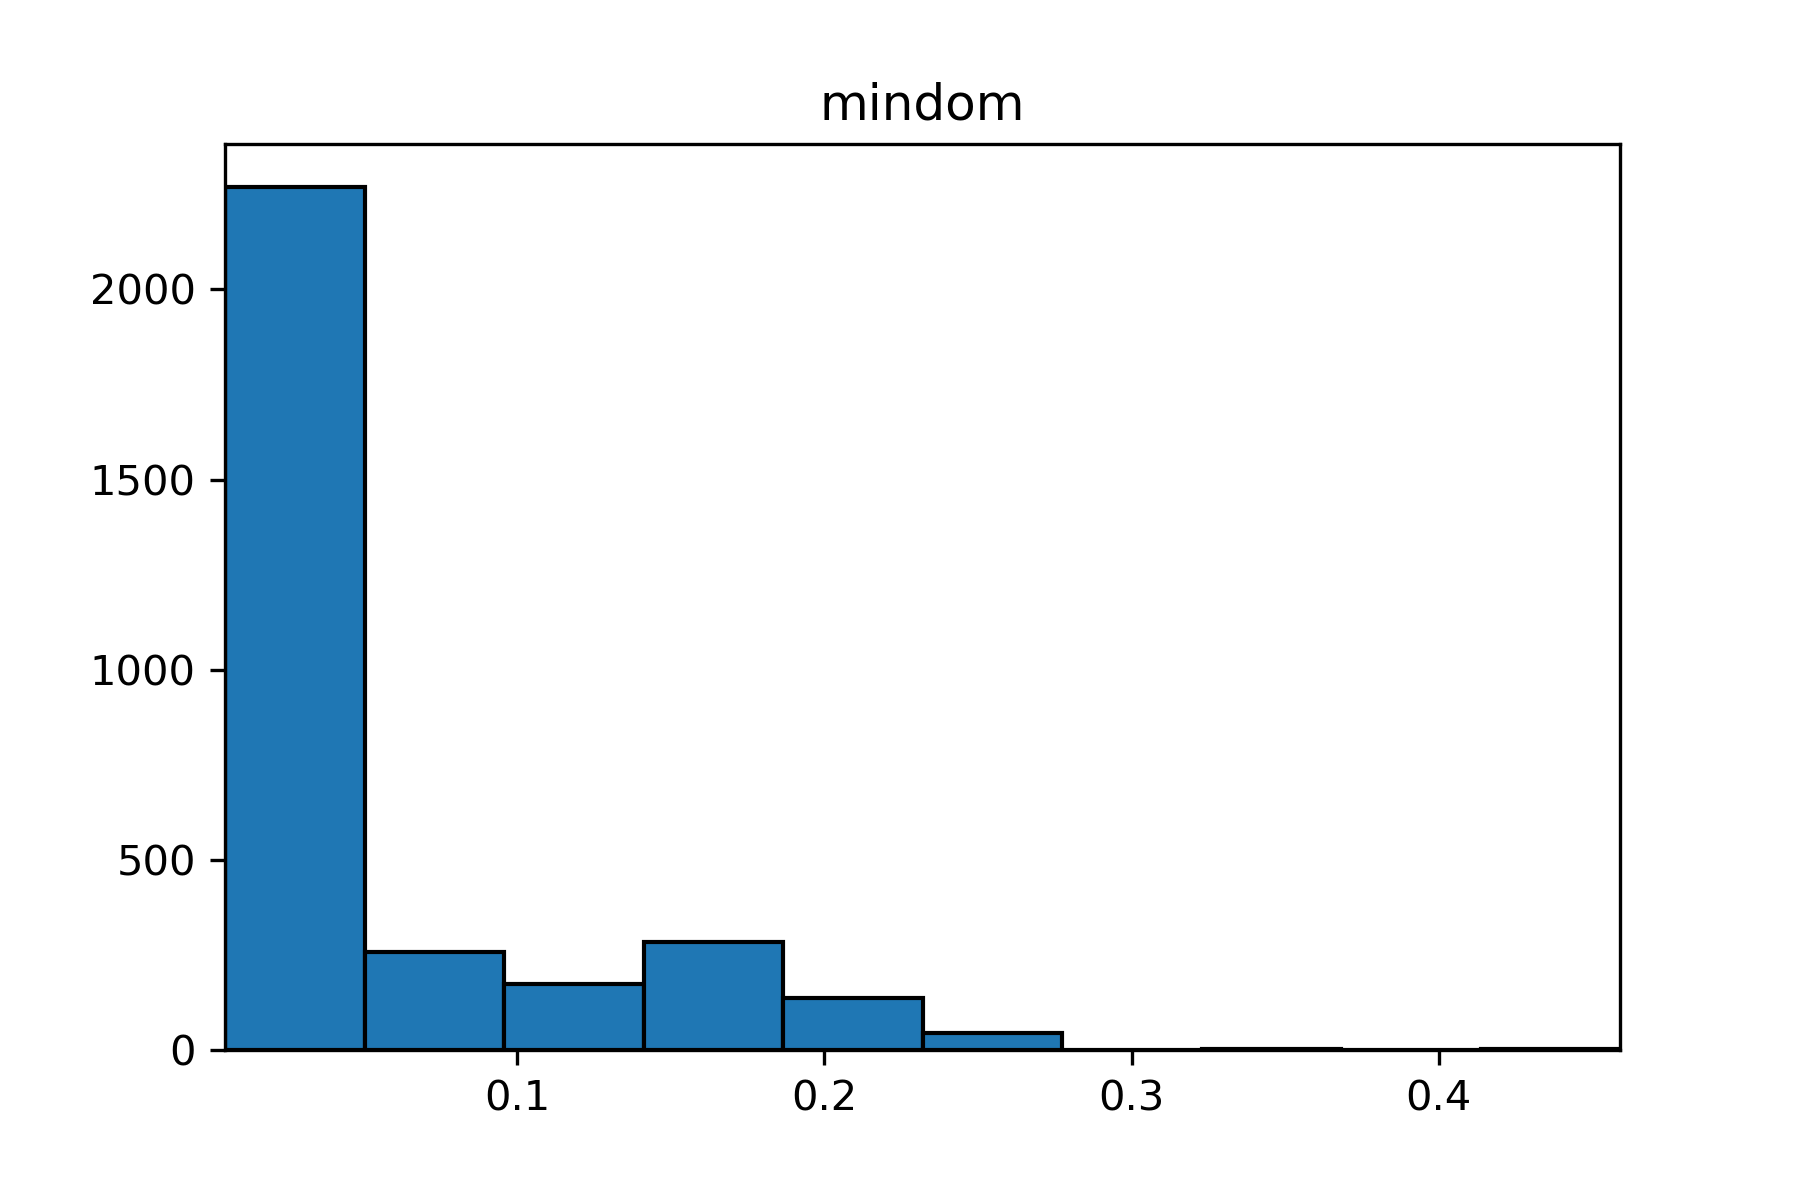
\includegraphics[width=3.85cm]{raw_15_mindom}
        \caption{mindom}
        \label{fig:sub_raw_16}
    \end{subfigure}\hfill
    % maxdom
    \begin{subfigure}{0.32\textwidth}
        \centering
        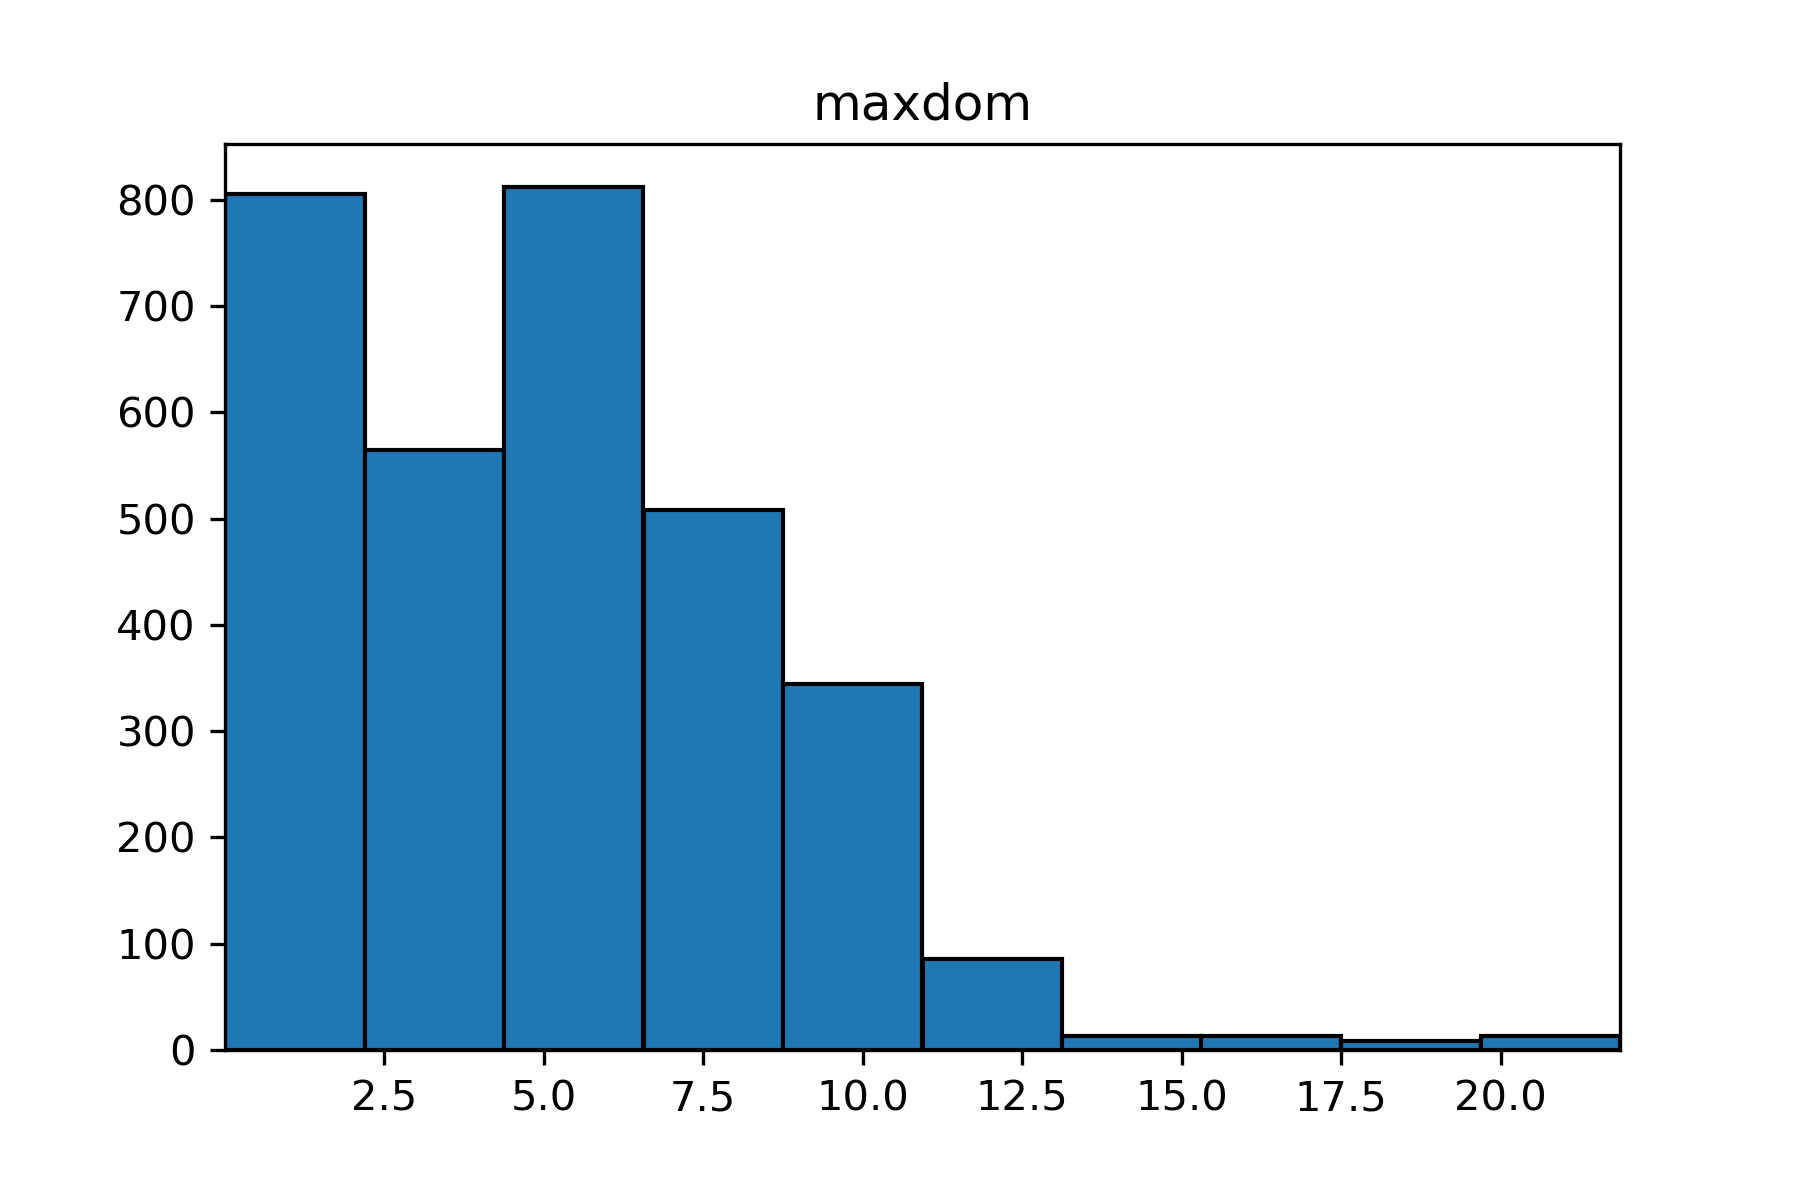
\includegraphics[width=3.85cm]{raw_16_maxdom}
        \caption{maxdom}
        \label{fig:sub_raw_17}
    \end{subfigure}\hfill
    % dfrange
    \begin{subfigure}{0.32\textwidth}
        \centering
        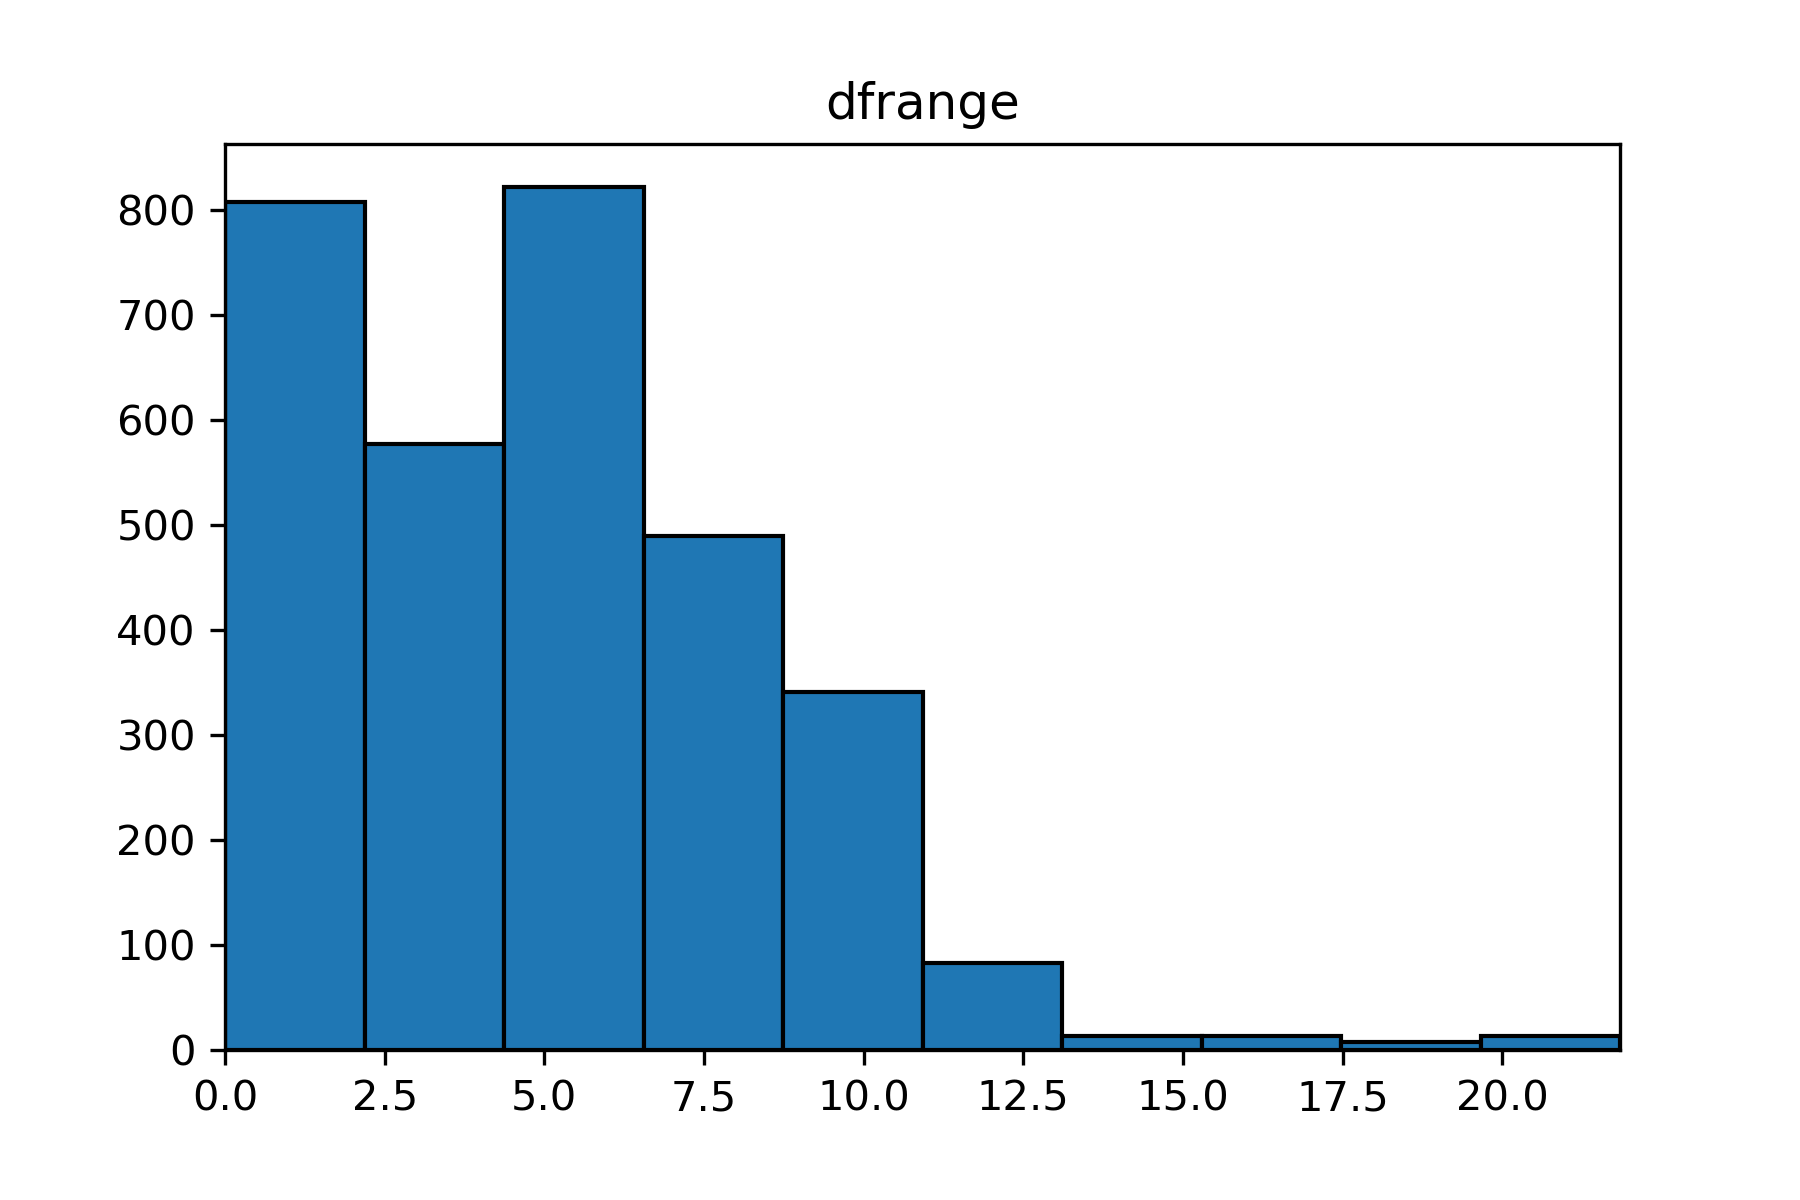
\includegraphics[width=3.85cm]{raw_17_dfrange}
        \caption{dfrange}
        \label{fig:sub_raw_18}
    \end{subfigure}\hfill
    % modindx
    \begin{subfigure}{0.32\textwidth}
        \centering
        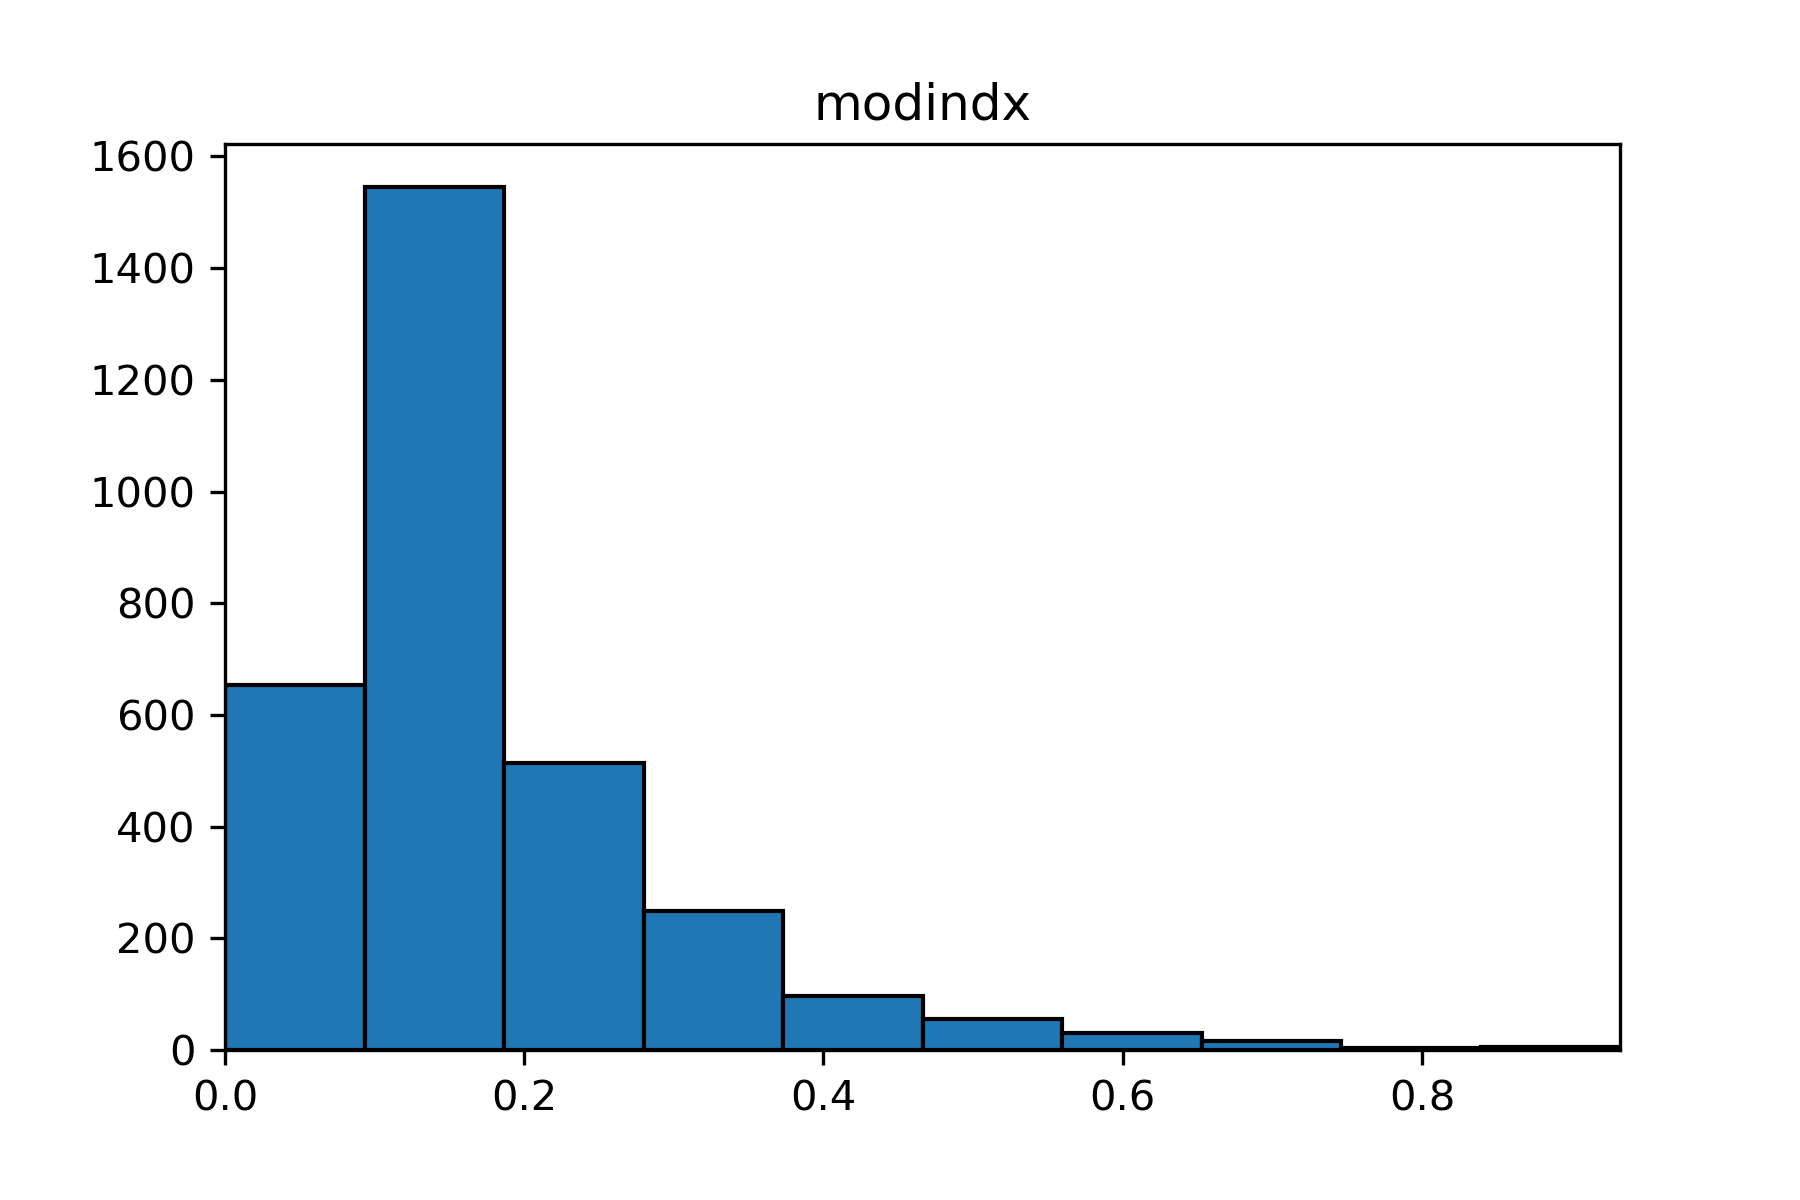
\includegraphics[width=3.85cm]{raw_18_modindx}
        \caption{modindx}
        \label{fig:sub_raw_19}
    \end{subfigure}
    % caption and label
    \caption{Histograms of raw input features}
    \label{fig:pre-ex1-raw_histograms}
\end{figure}

% histograms of stardardized features

\begin{figure}
    \centering
    % sd
    \begin{subfigure}{0.32\textwidth}
        \centering
        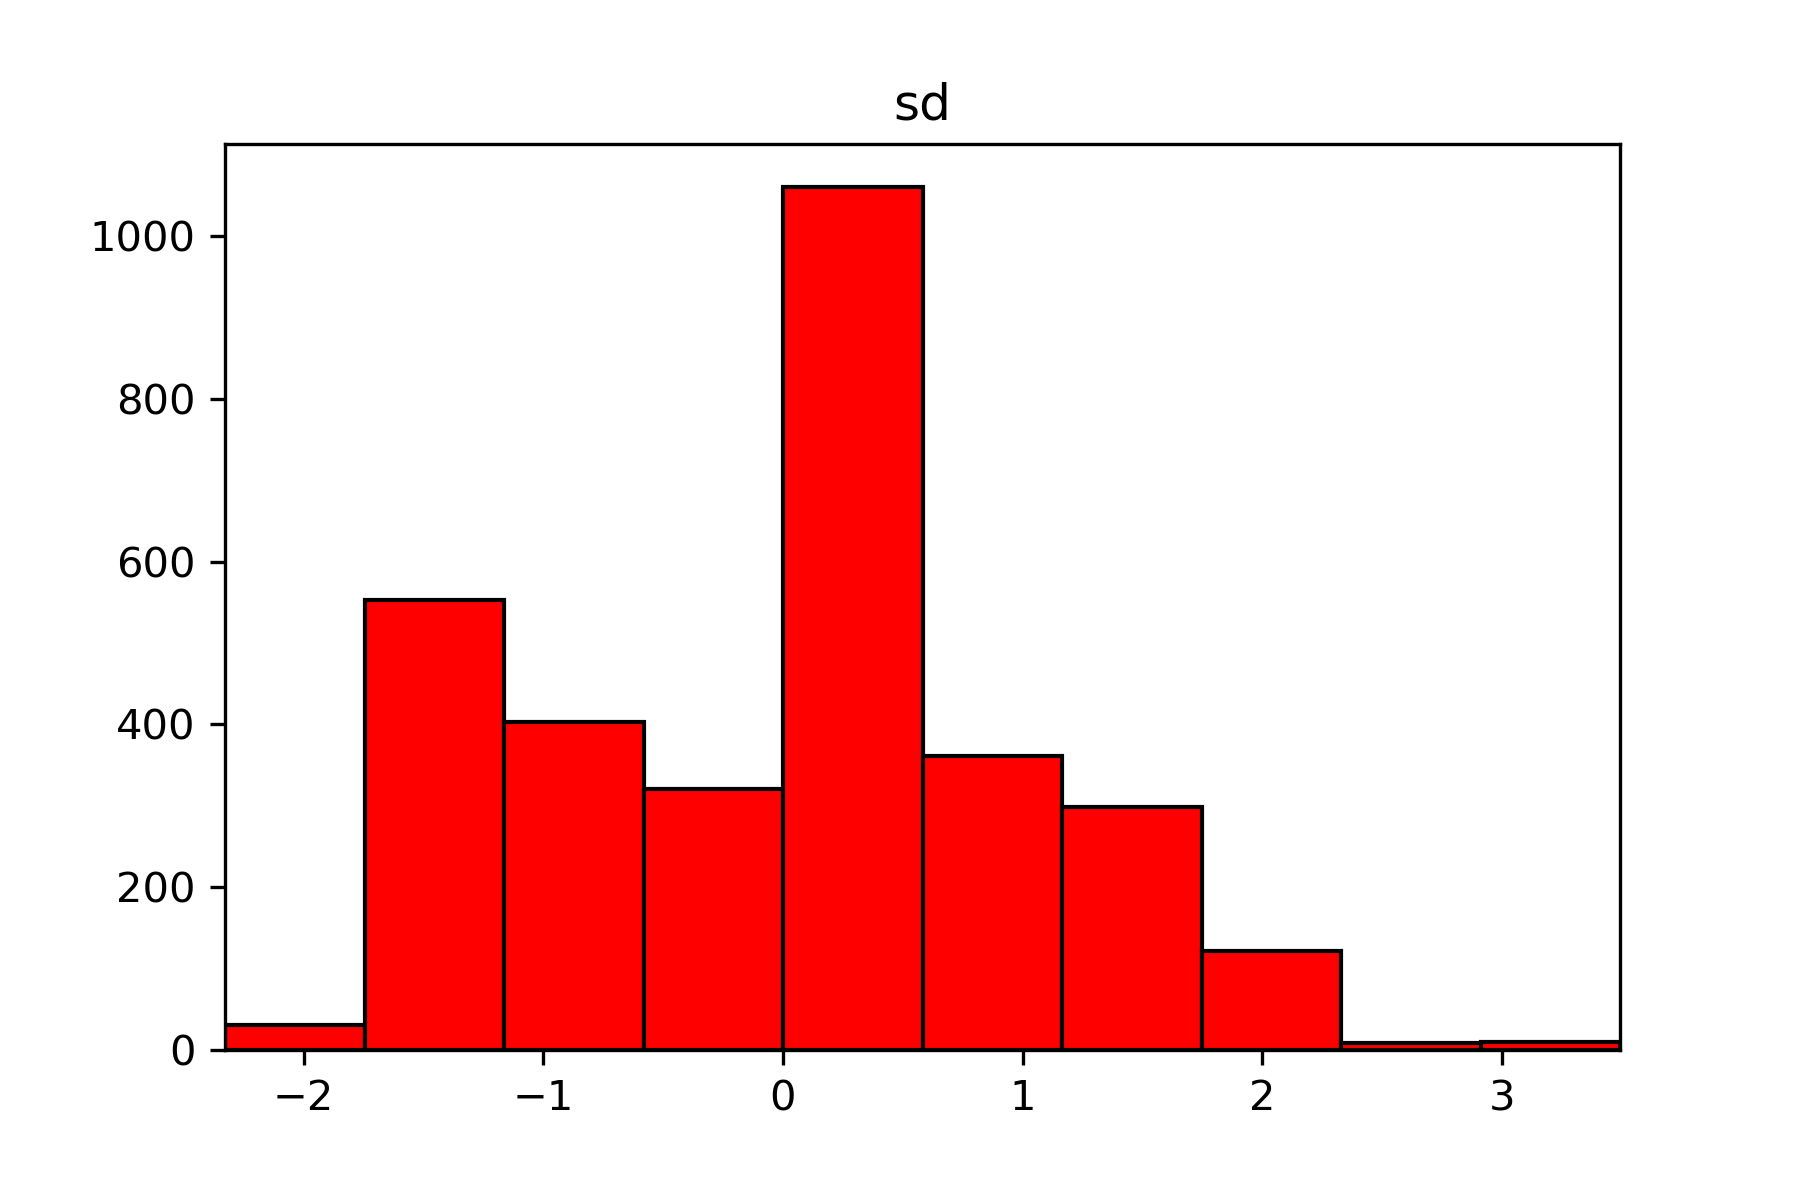
\includegraphics[width=3.85cm]{std_0_sd}
        \caption{sd}
        \label{fig:sub_std_1}
    \end{subfigure}
    \hfill
    % median
    \begin{subfigure}{0.32\textwidth}
        \centering
        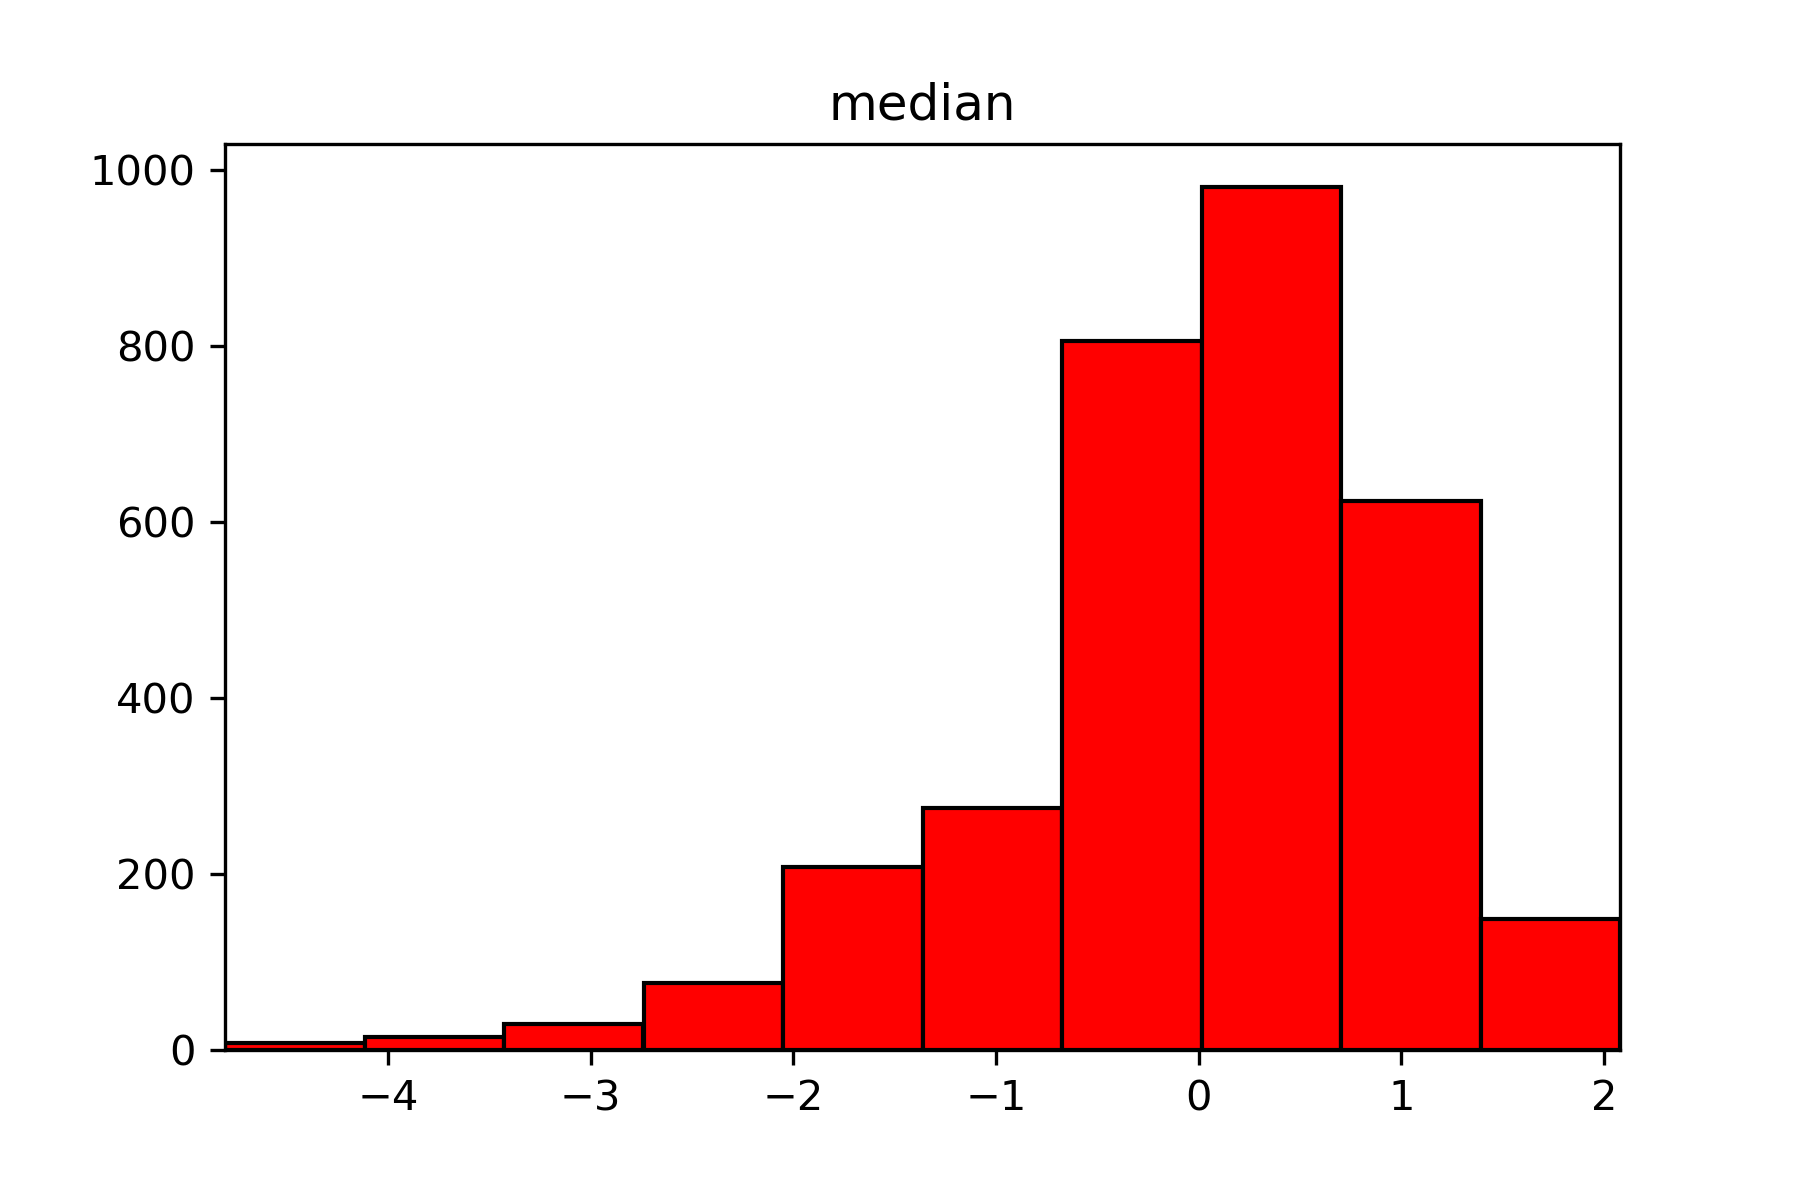
\includegraphics[width=3.85cm]{std_1_median}
        \caption{median}
        \label{fig:sub_std_2}
    \end{subfigure}
    \hfill
    % Q25
    \begin{subfigure}{0.32\textwidth}
        \centering
        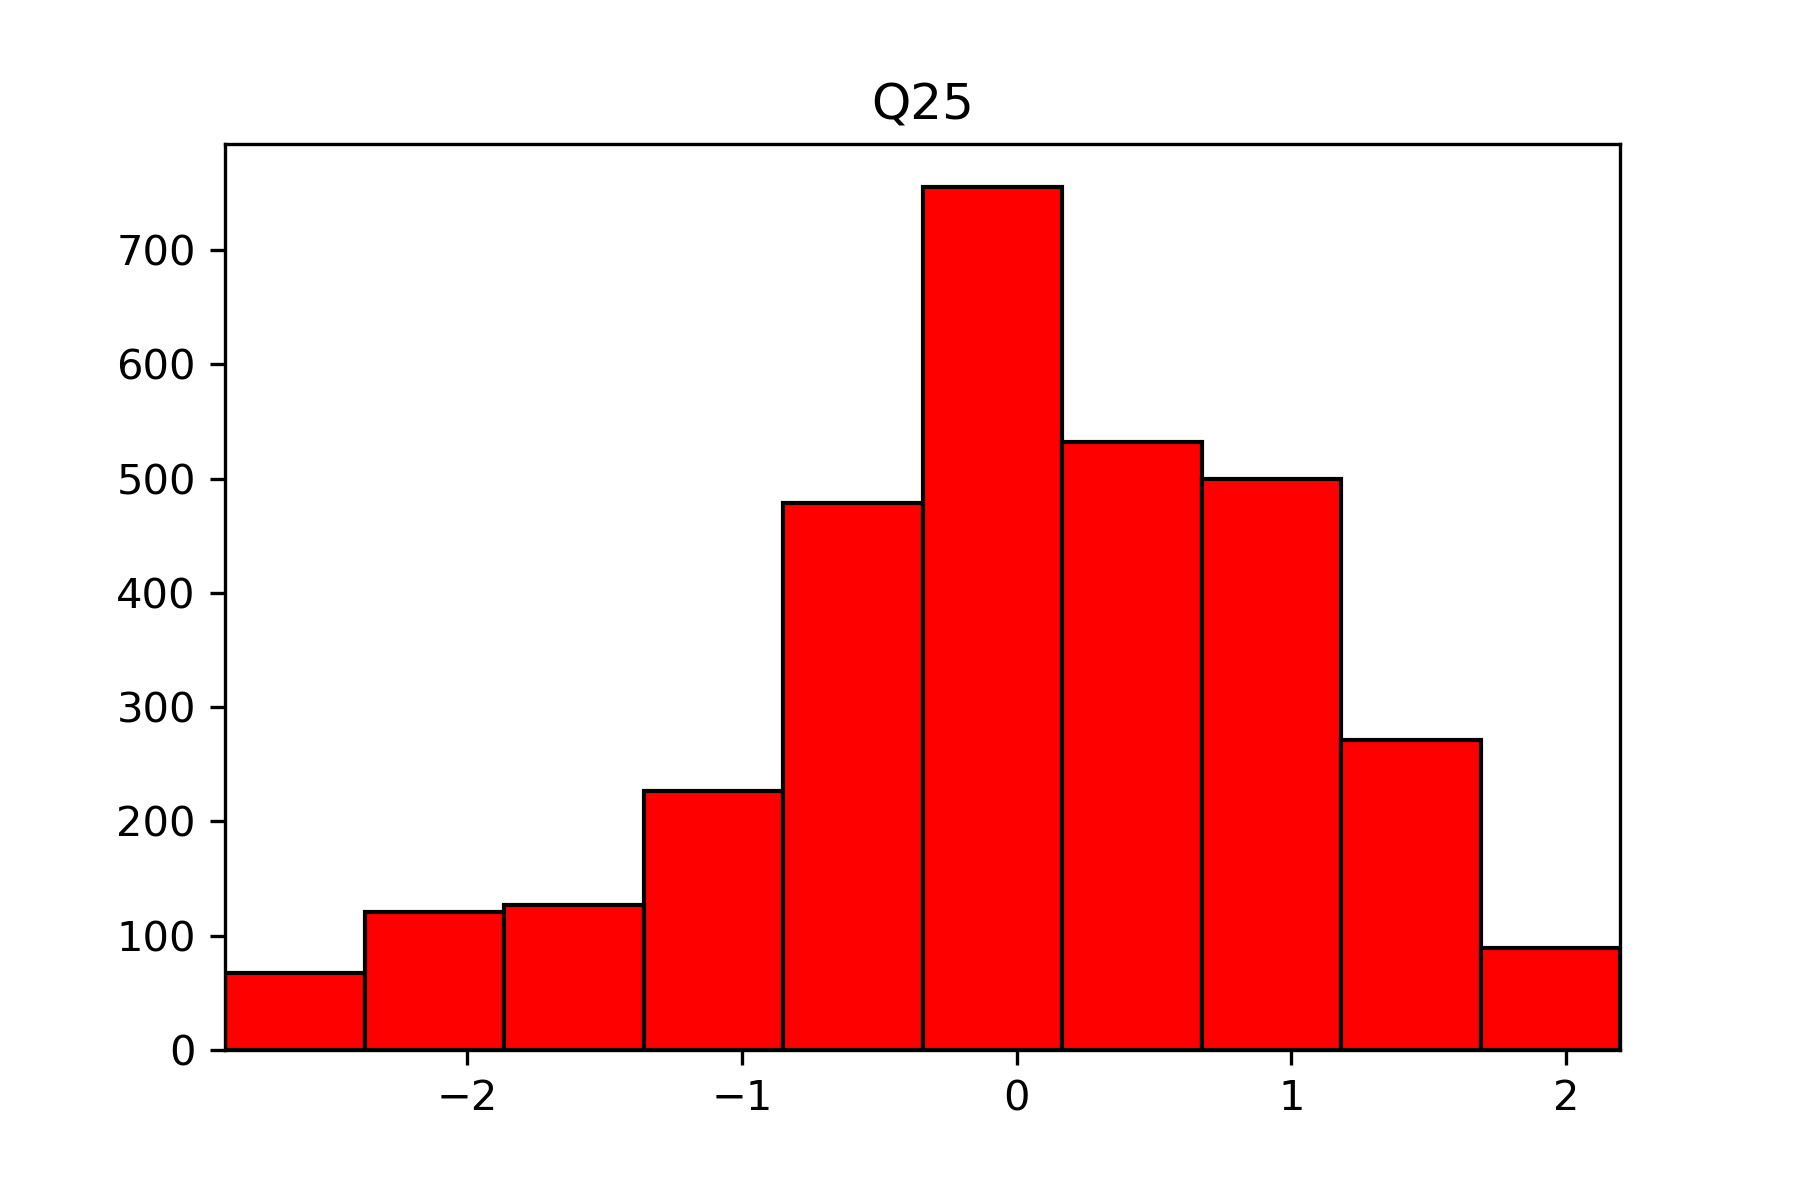
\includegraphics[width=3.85cm]{std_2_Q25}
        \caption{Q25}
        \label{fig:sub_std_3}
    \end{subfigure}%
    \\
    % Q75
    \begin{subfigure}{0.32\textwidth}
        \centering
        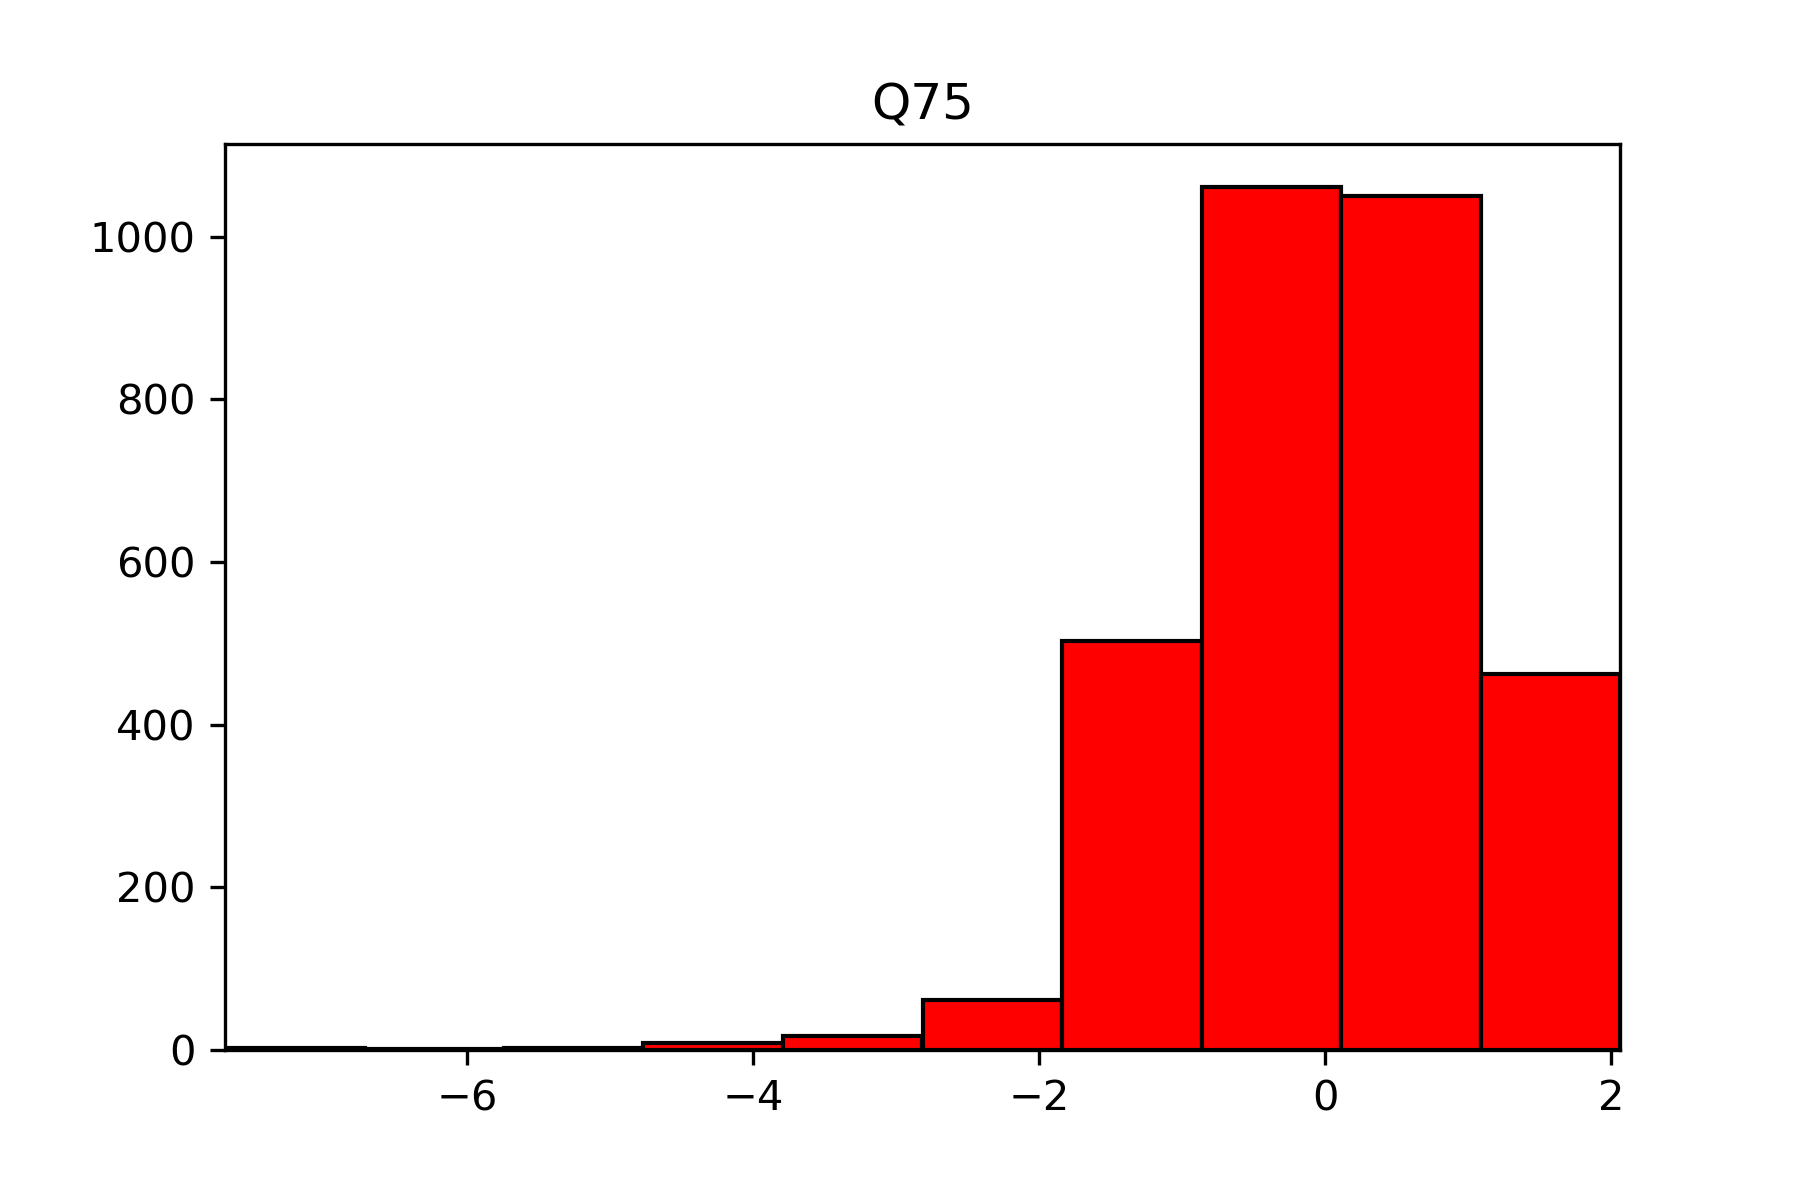
\includegraphics[width=3.85cm]{std_3_Q75}
        \caption{Q75}
        \label{fig:sub_std_4}
    \end{subfigure}\hfill
    % Q75
    \begin{subfigure}{0.32\textwidth}
        \centering
        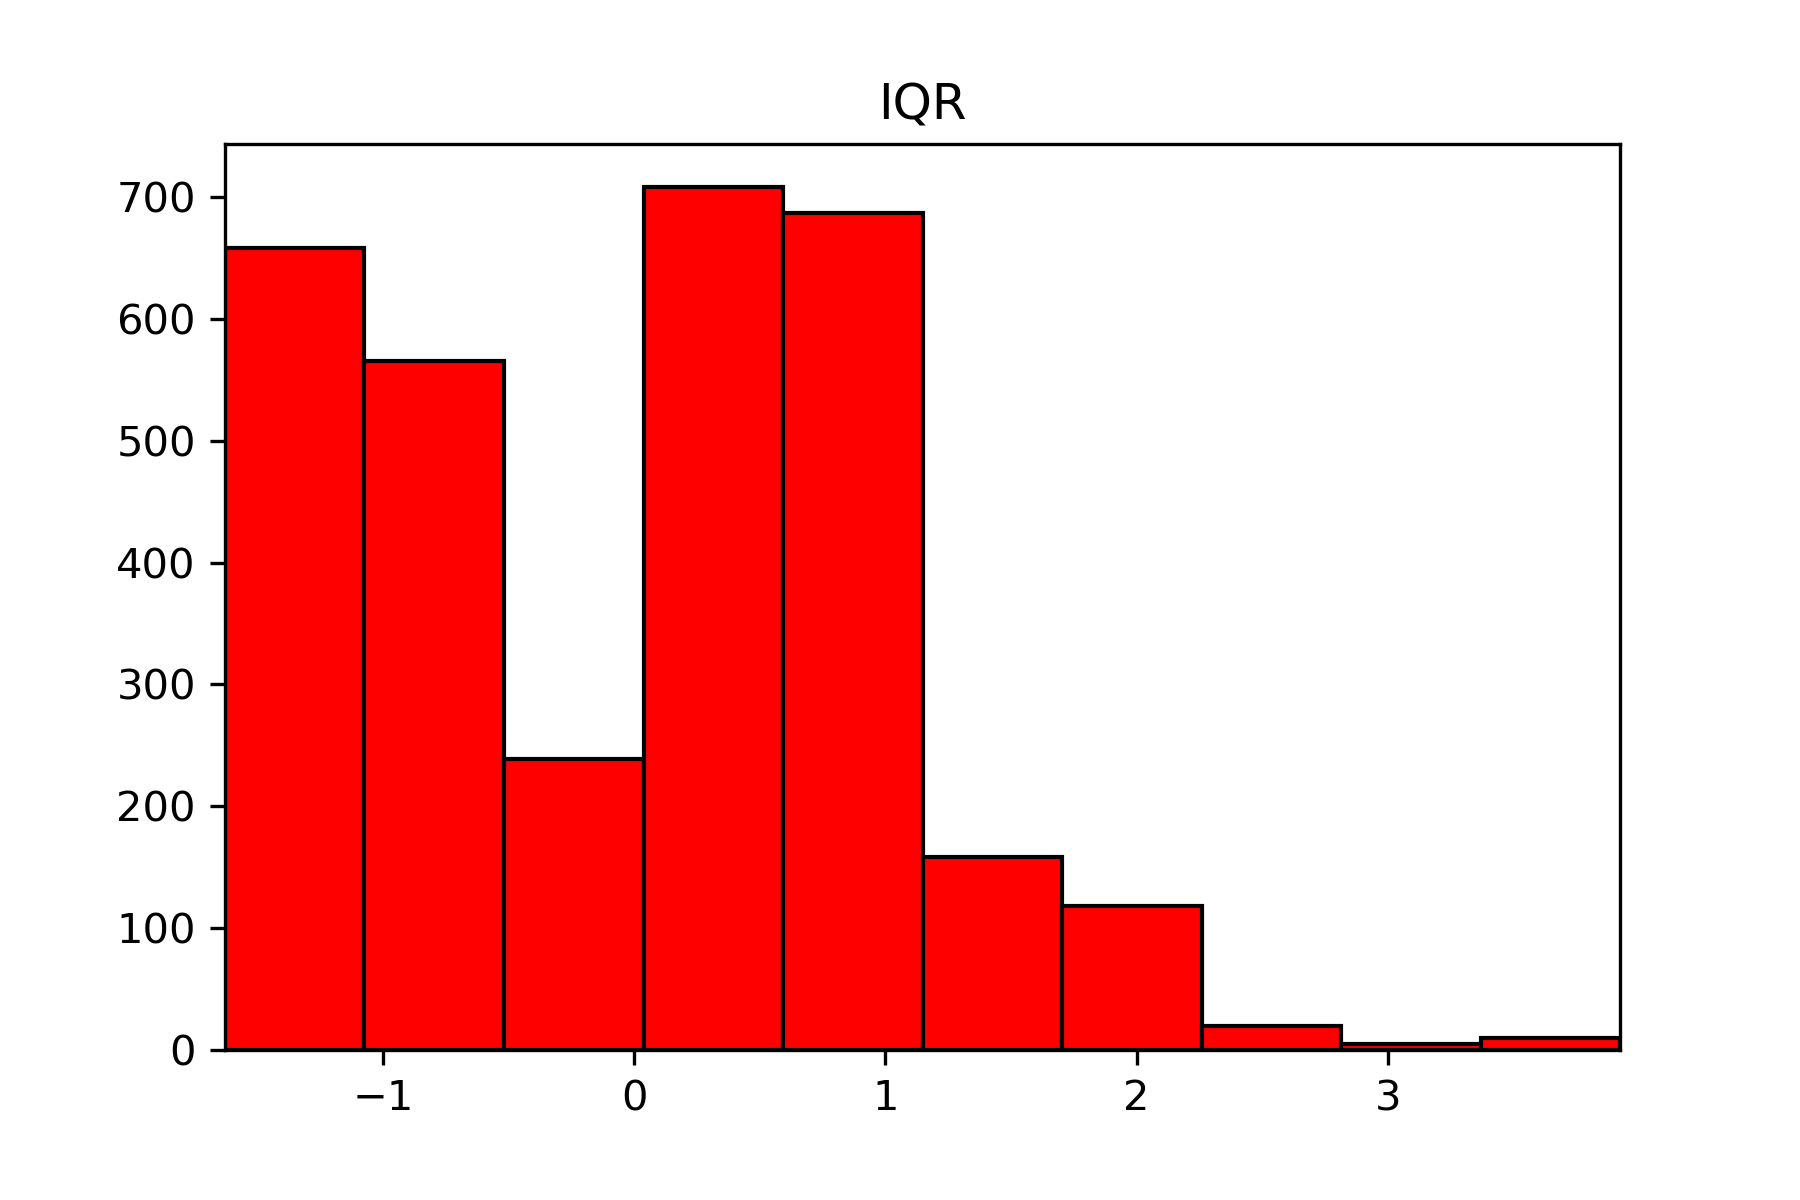
\includegraphics[width=3.85cm]{std_4_IQR}
        \caption{IQR}
        \label{fig:sub_std_5}
    \end{subfigure}\hfill
    % skew
    \begin{subfigure}{0.32\textwidth}
        \centering
        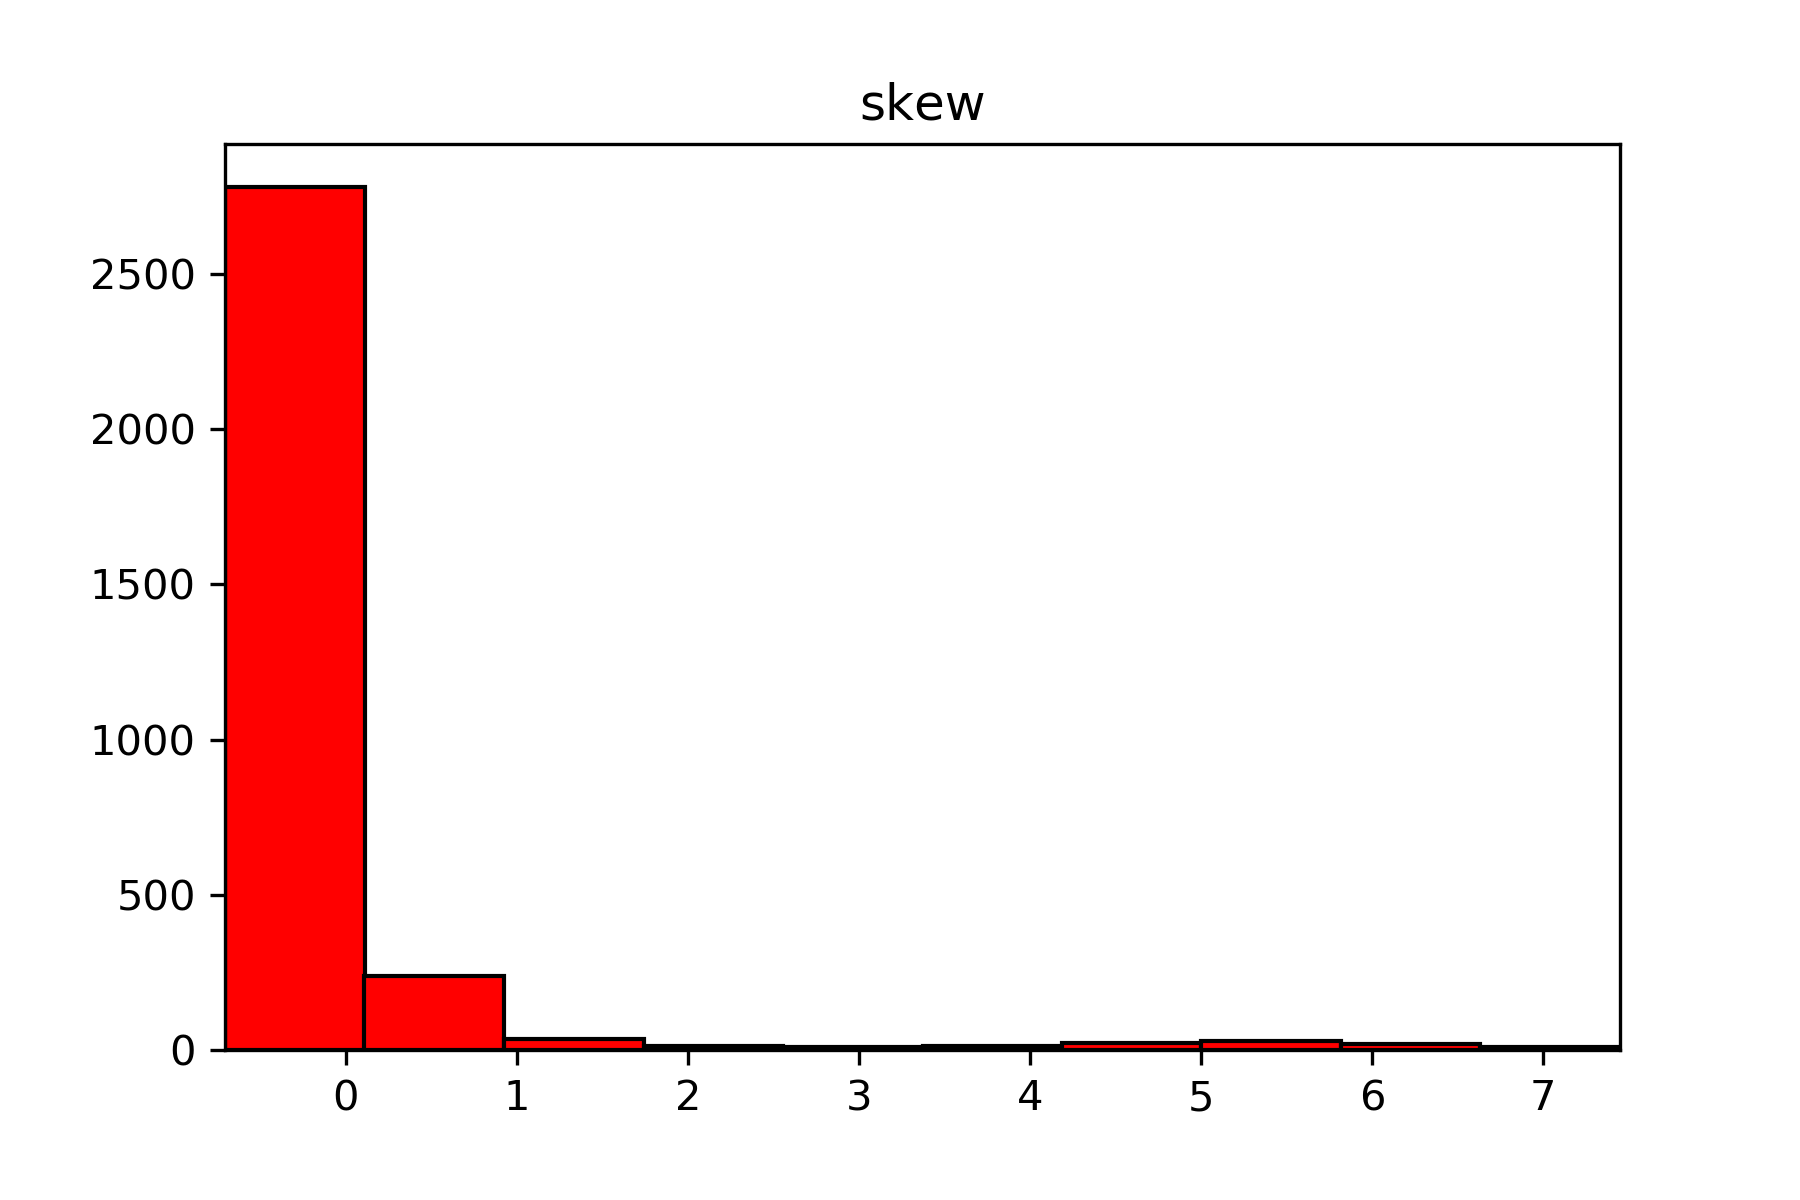
\includegraphics[width=3.85cm]{std_5_skew}
        \caption{skew}
        \label{fig:sub_std_6}
    \end{subfigure}
    \\
    % kurt
    \begin{subfigure}{0.32\textwidth}
        \centering
        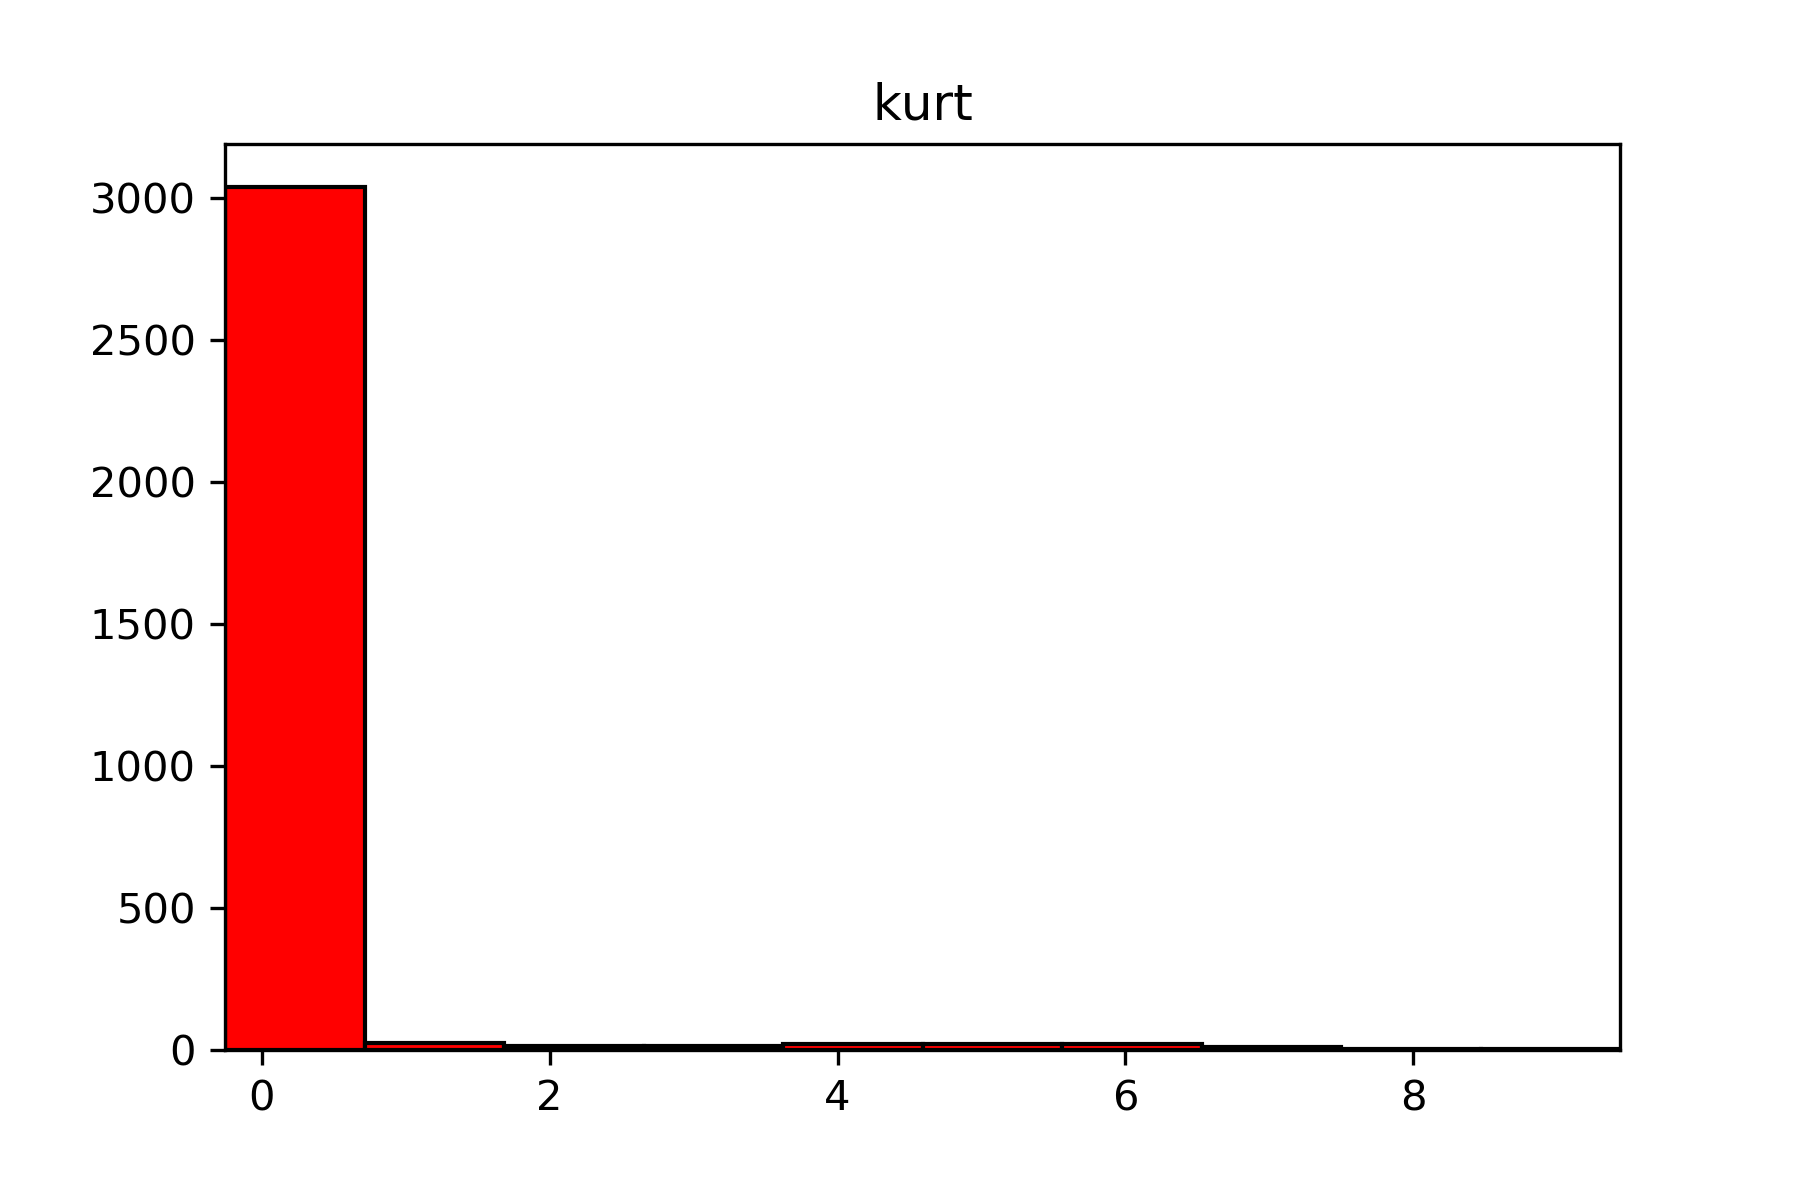
\includegraphics[width=3.85cm]{std_6_kurt}
        \caption{kurt}
        \label{fig:sub_std_7}
    \end{subfigure}\hfill
    % sp ent
    \begin{subfigure}{0.32\textwidth}
        \centering
        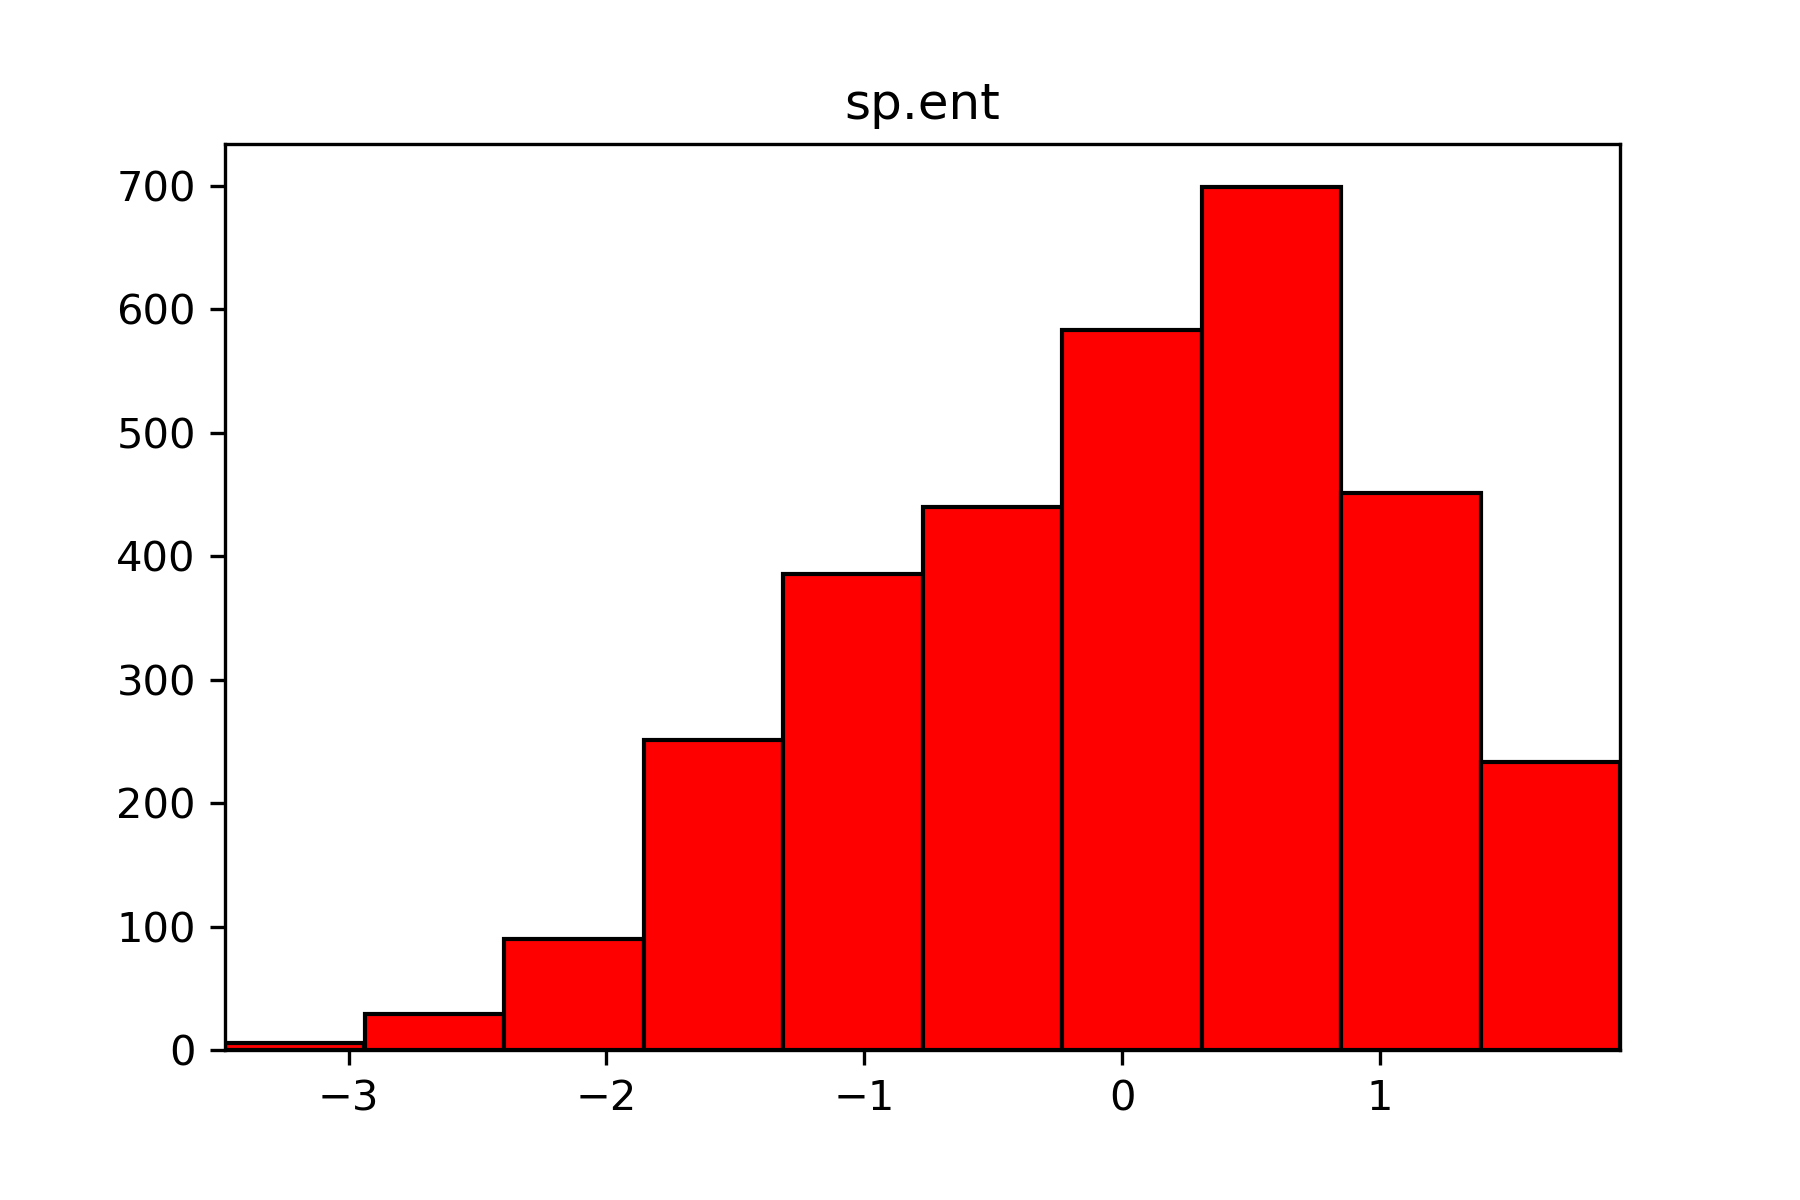
\includegraphics[width=3.85cm]{std_7_sp_ent}
        \caption{sp ent}
        \label{fig:sub_std_8}
    \end{subfigure}\hfill
    % sfm
    \begin{subfigure}{0.32\textwidth}
        \centering
        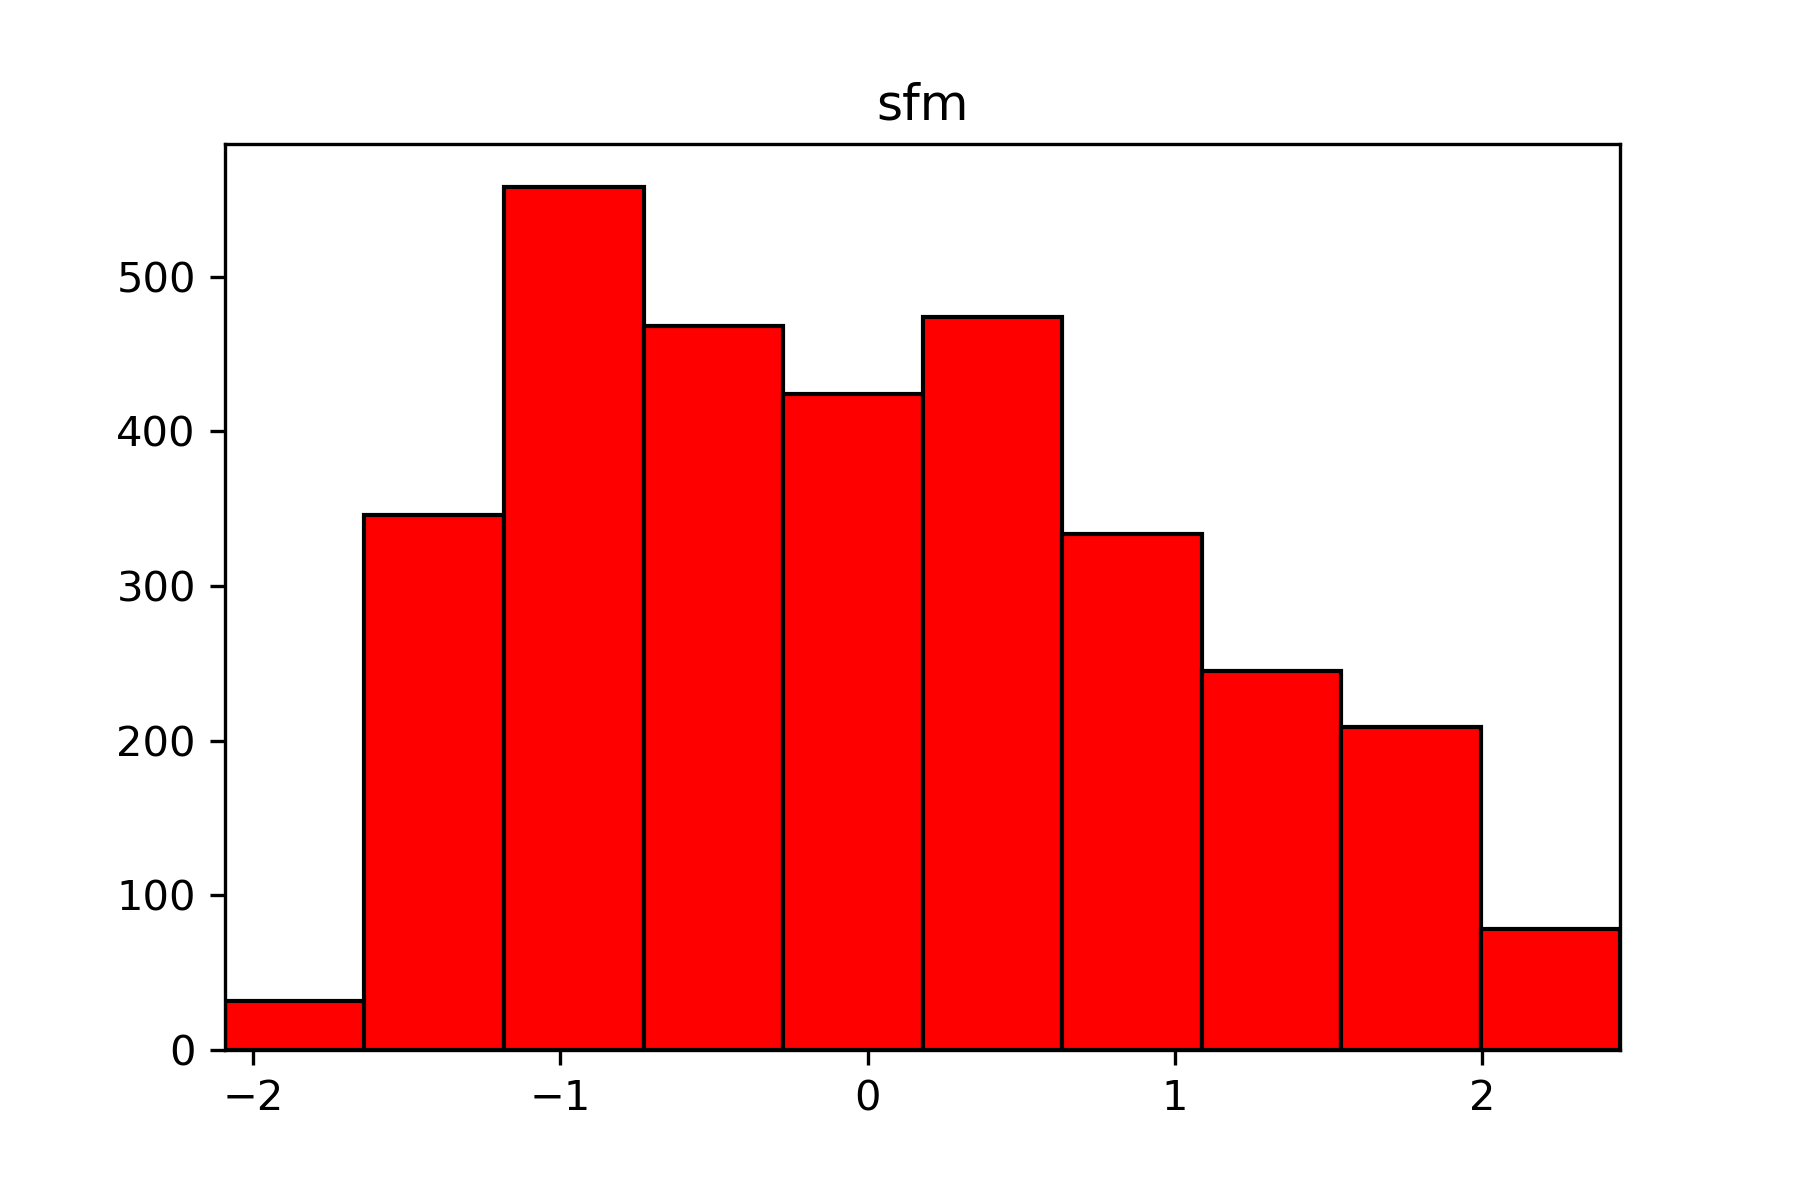
\includegraphics[width=3.85cm]{std_8_sfm}
        \caption{smf}
        \label{fig:sub_std_9}
    \end{subfigure}\hfill
    % mode
    \begin{subfigure}{0.32\textwidth}
        \centering
        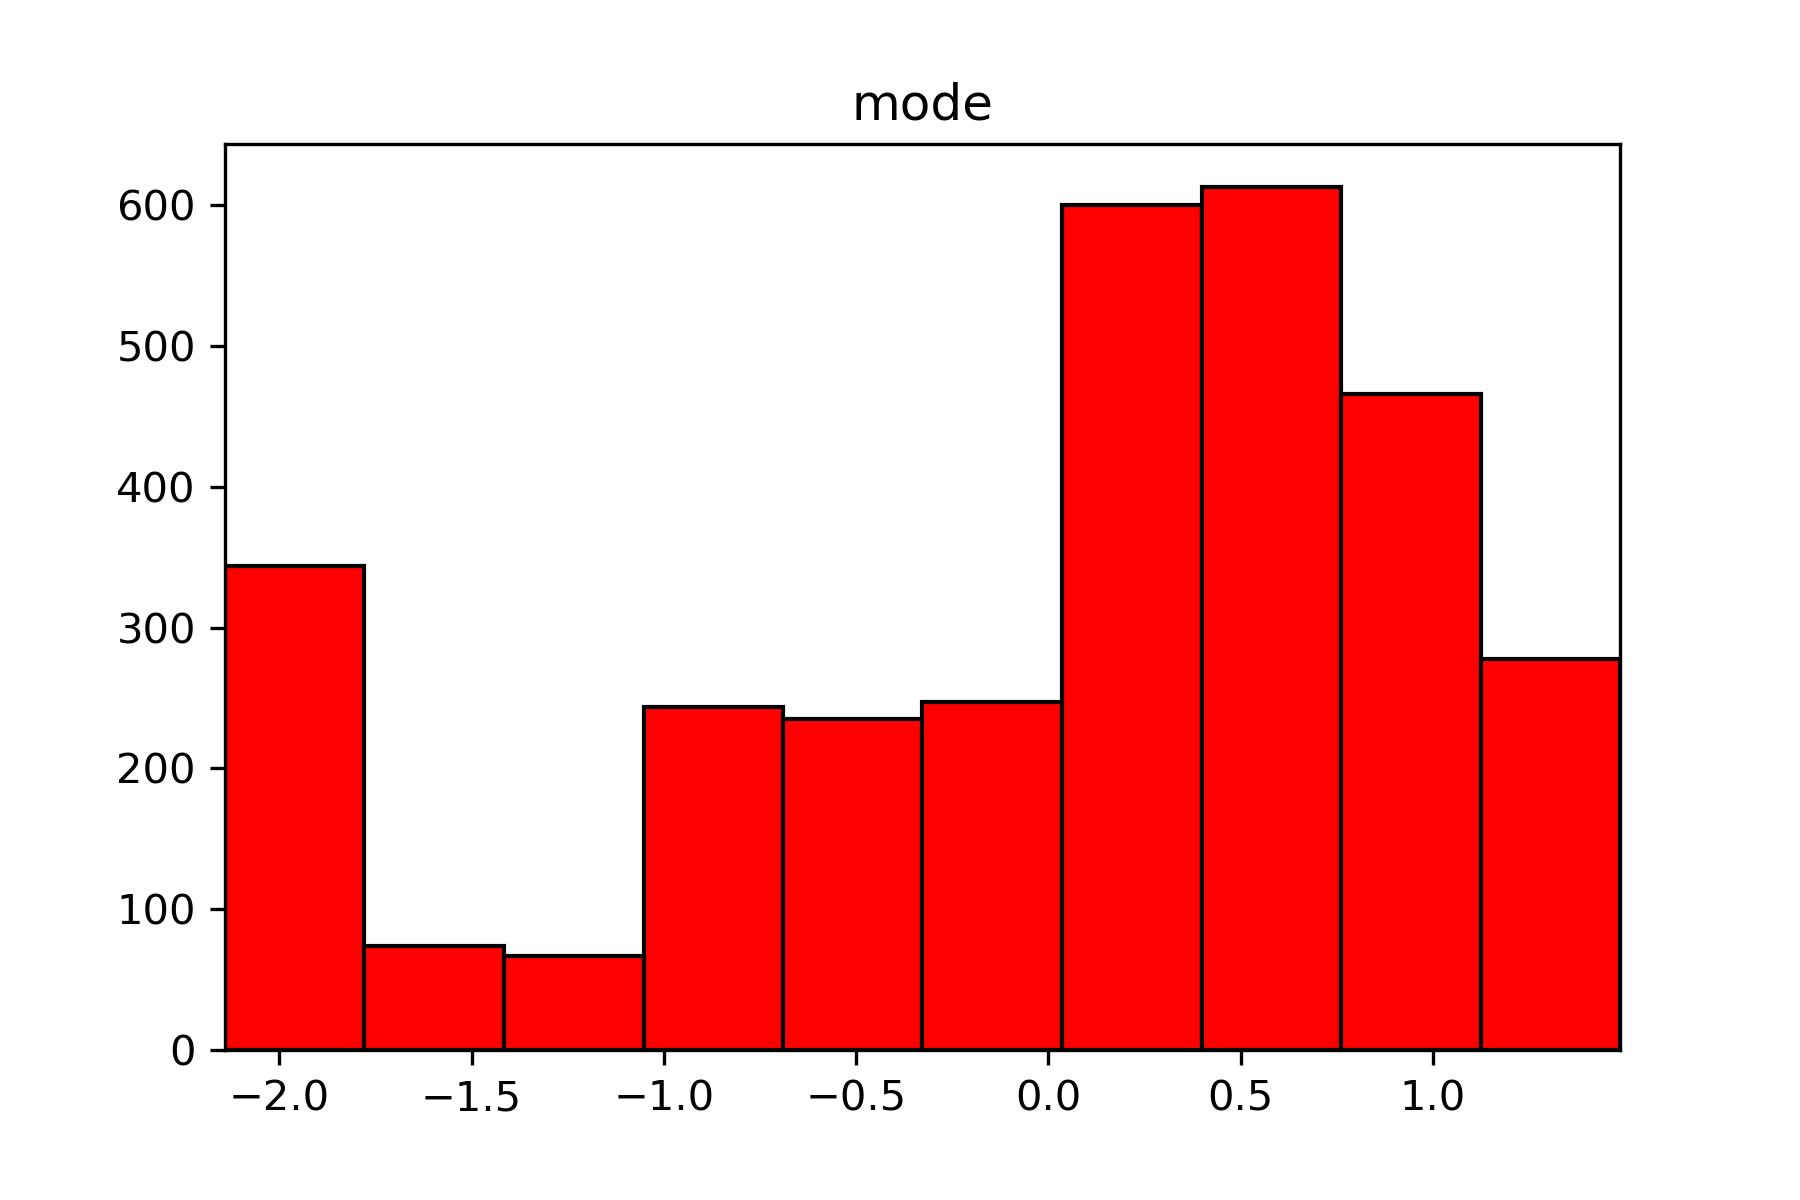
\includegraphics[width=3.85cm]{std_9_mode}
        \caption{mode}
        \label{fig:sub_std_10}
    \end{subfigure}\hfill
    % centroid
    \begin{subfigure}{0.32\textwidth}
        \centering
        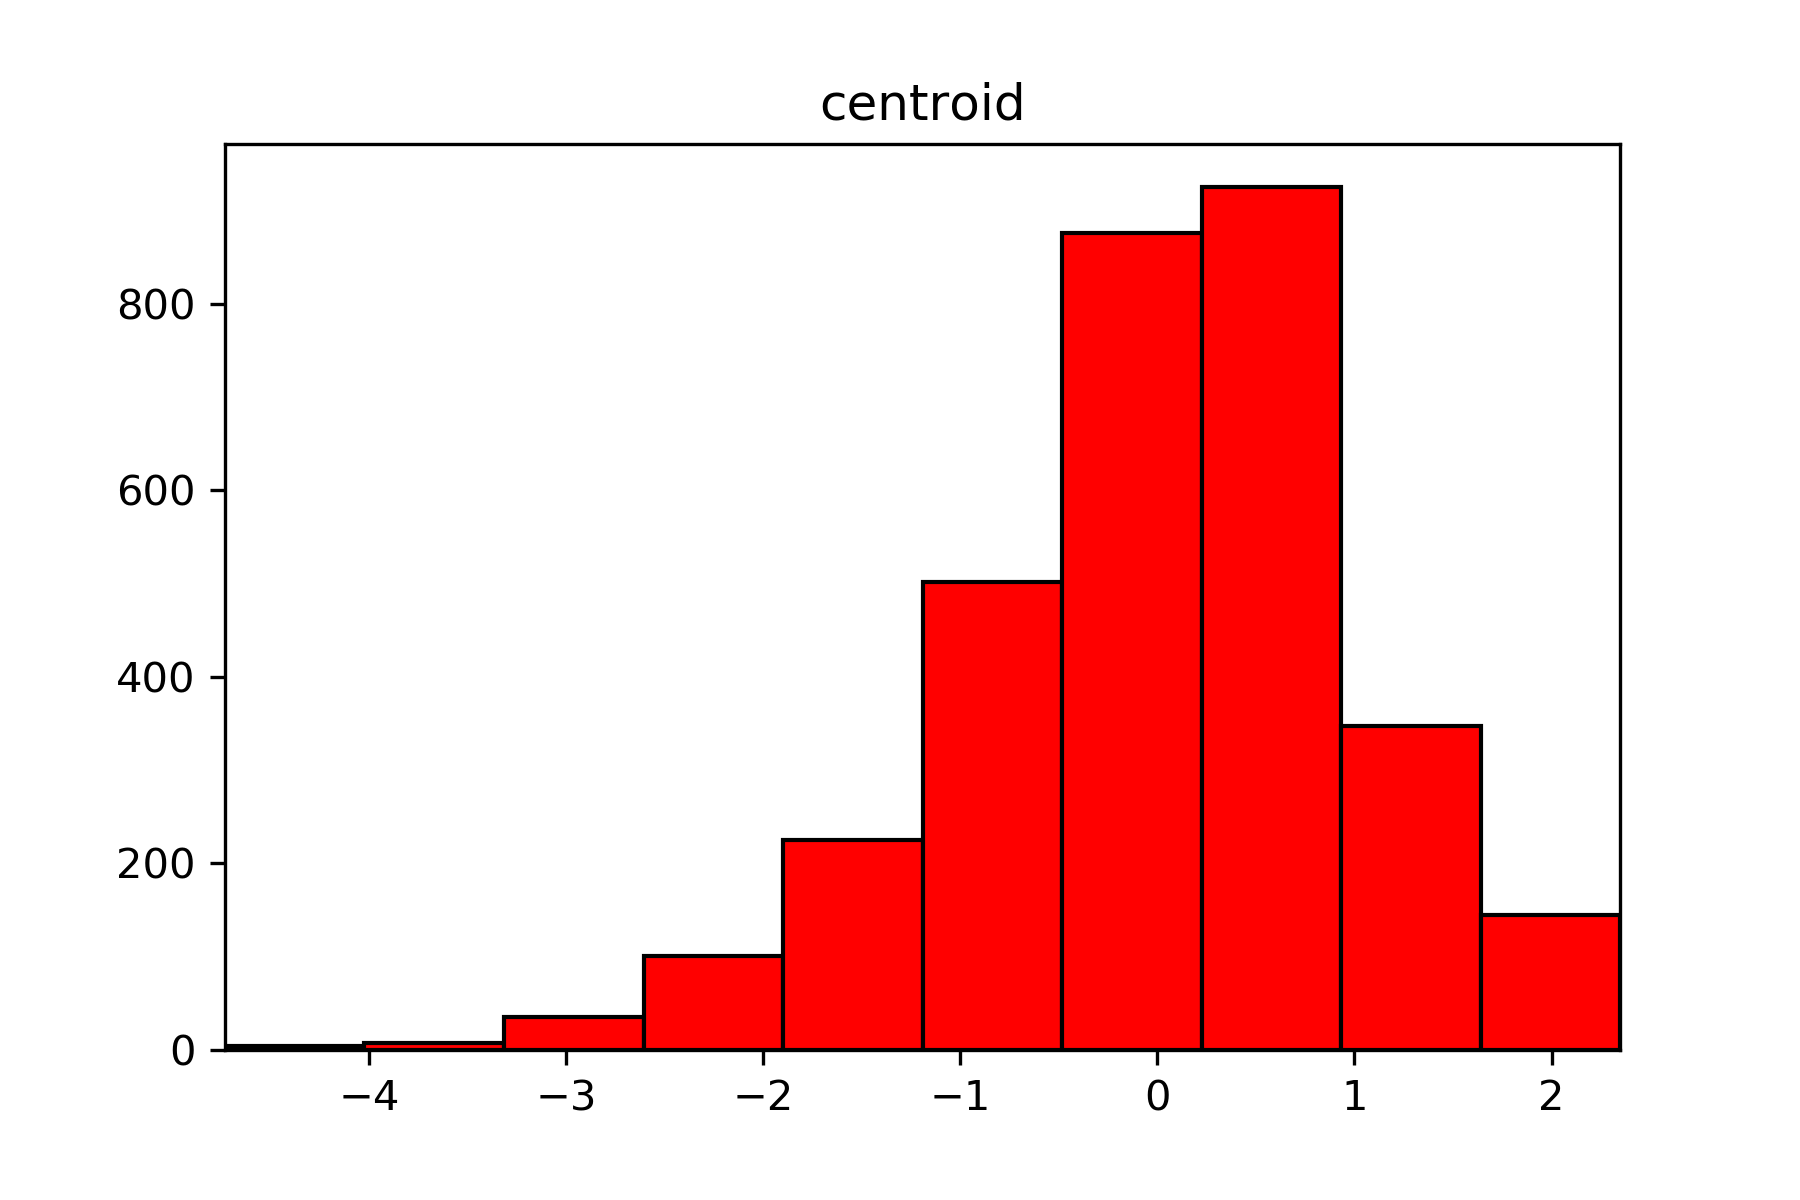
\includegraphics[width=3.85cm]{std_10_centroid}
        \caption{centroid}
        \label{fig:sub_std_11}
    \end{subfigure}\hfill
    % meanfun
    \begin{subfigure}{0.32\textwidth}
        \centering
        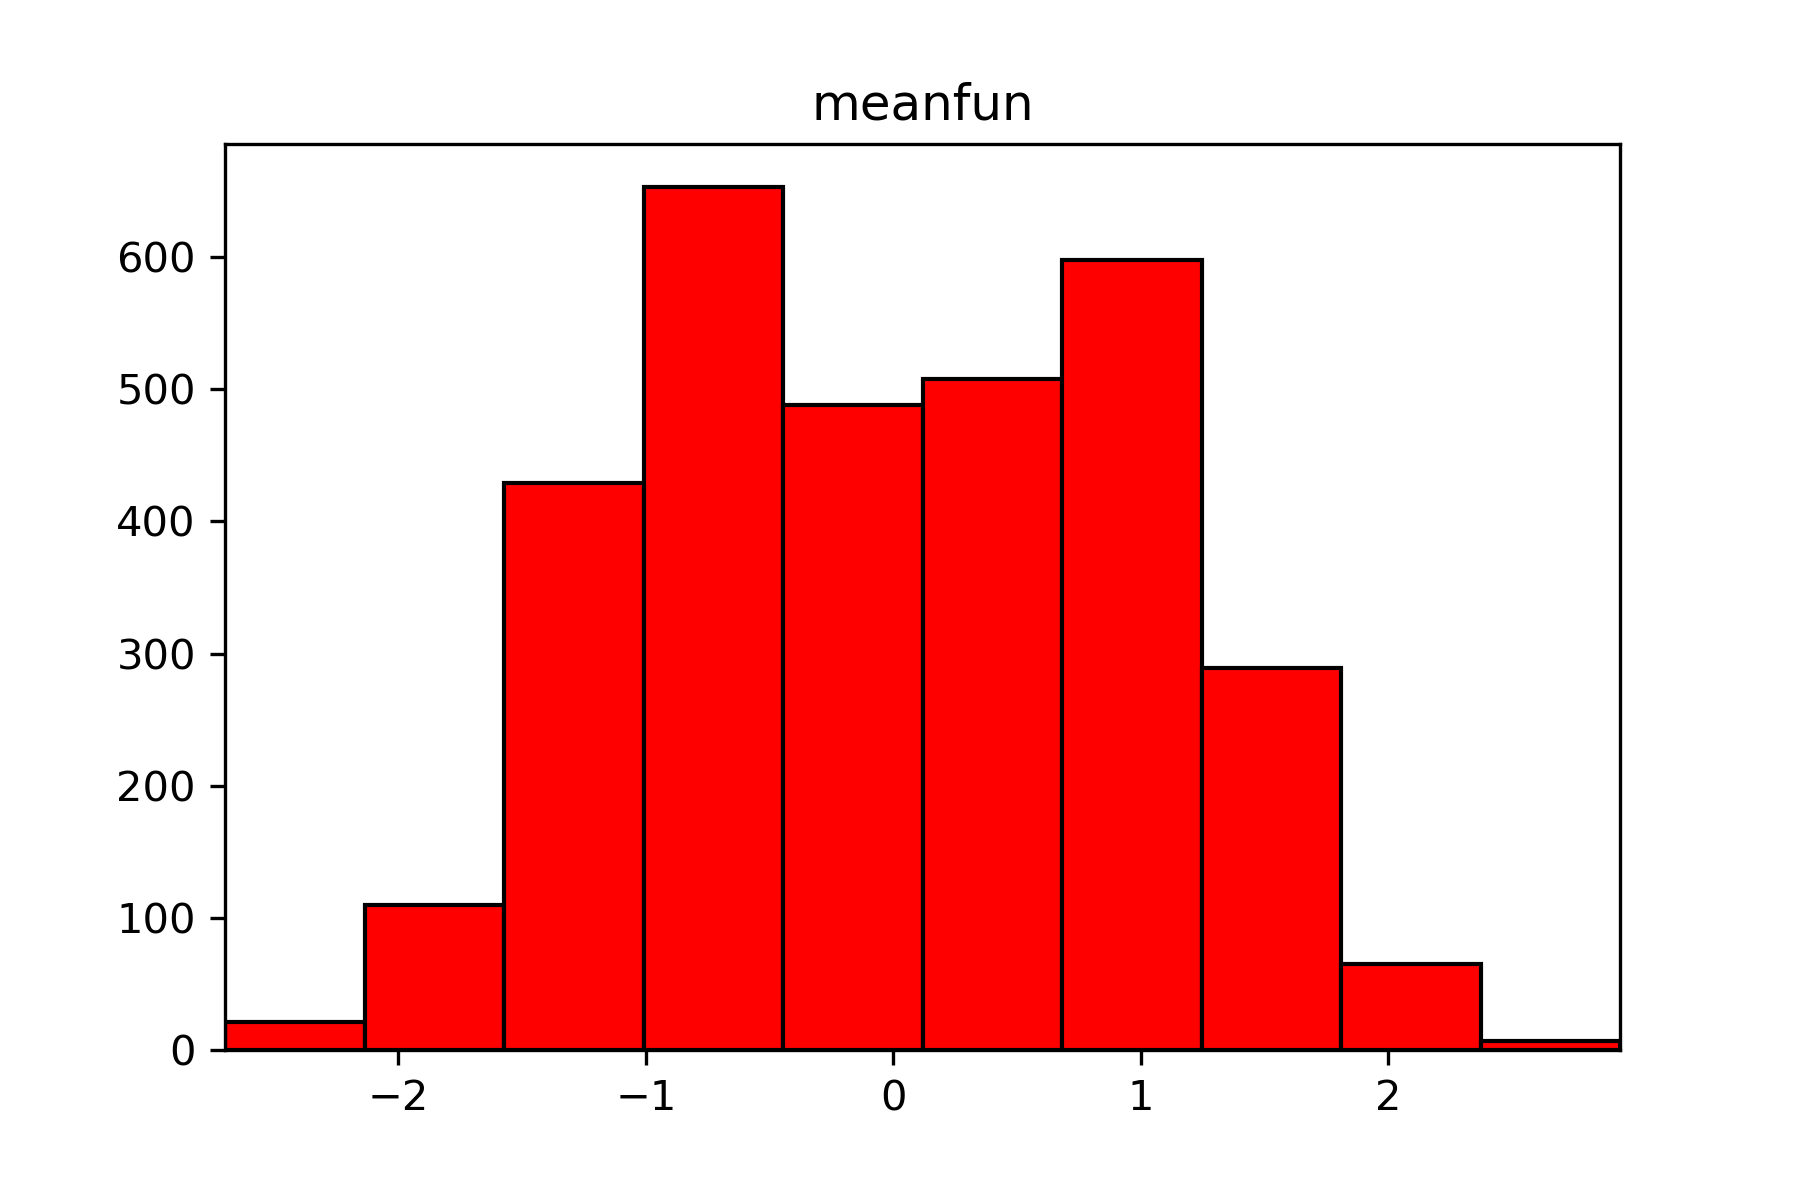
\includegraphics[width=3.85cm]{std_11_meanfun}
        \caption{meanfun}
        \label{fig:sub_std_12}
    \end{subfigure}\hfill
    % minfun
    \begin{subfigure}{0.32\textwidth}
        \centering
        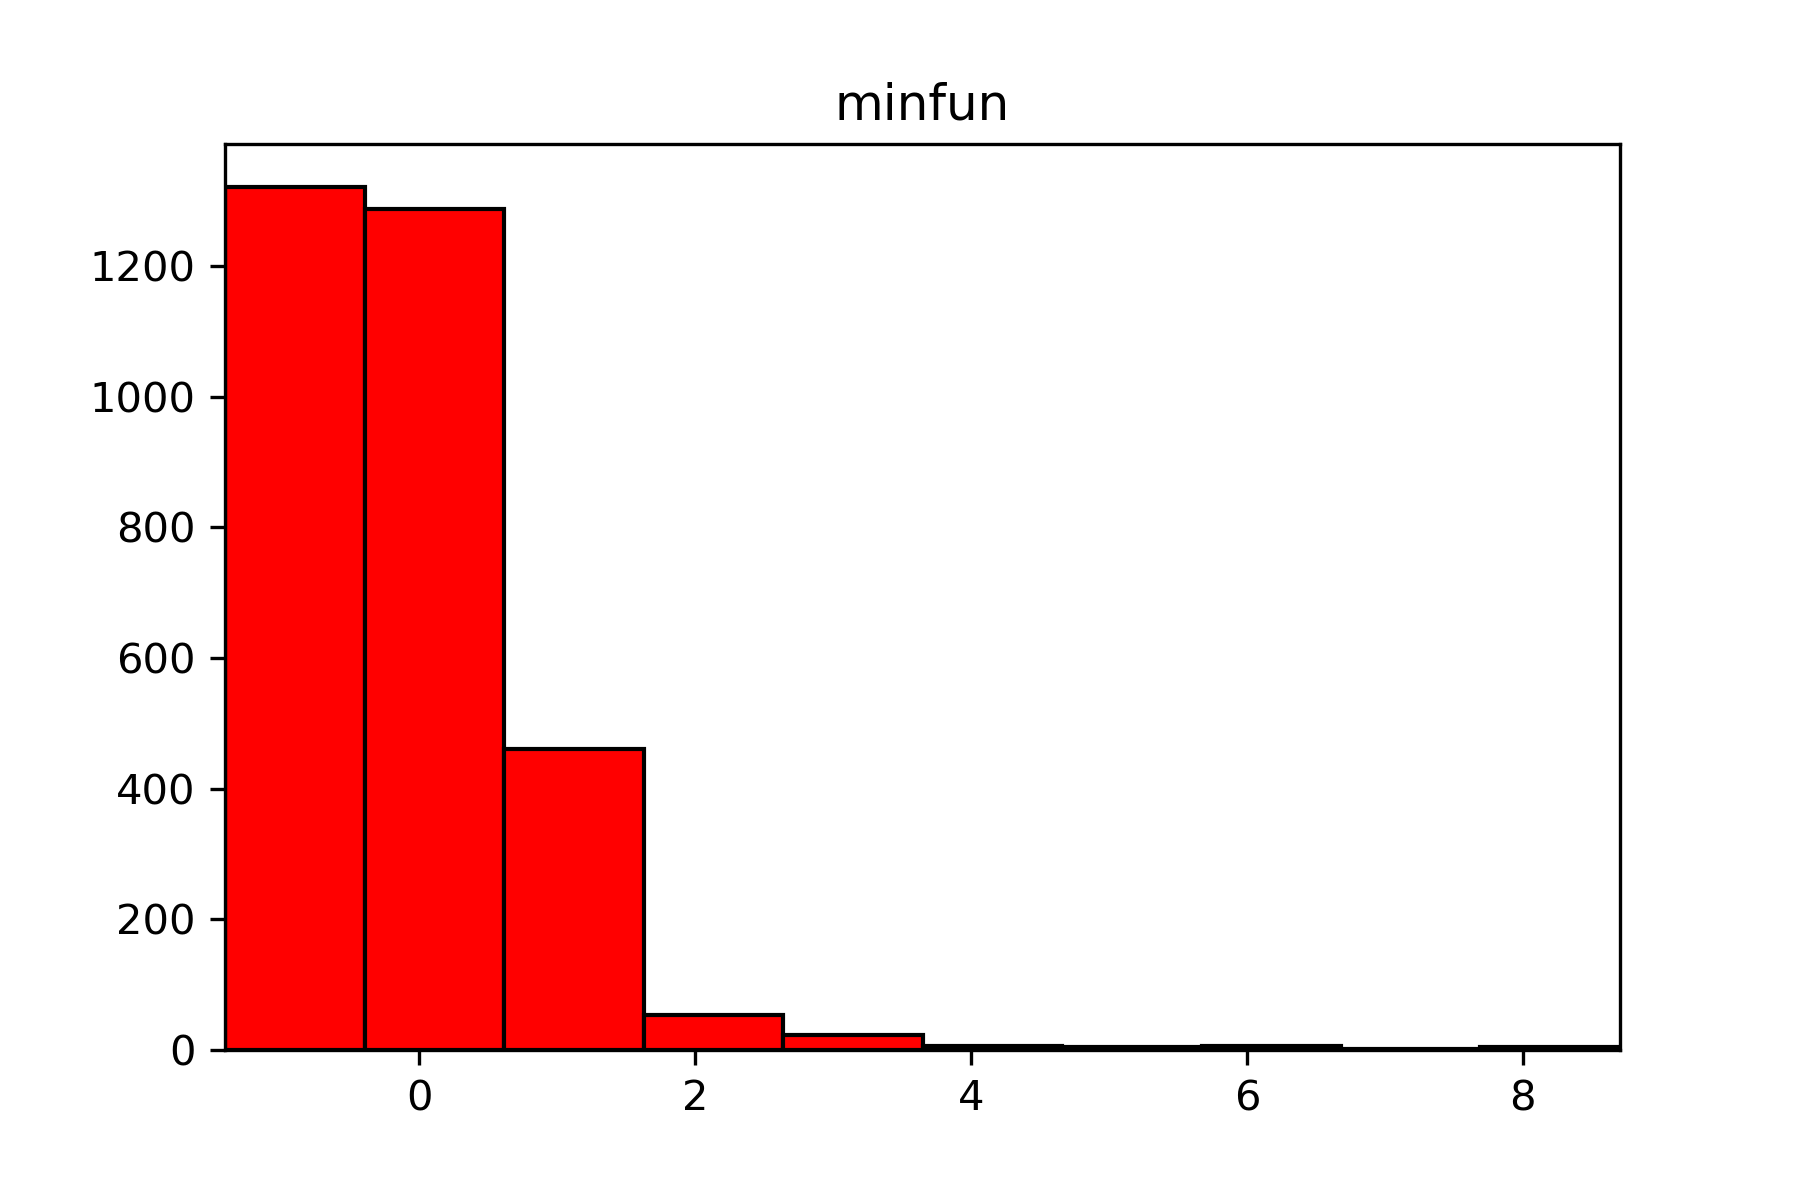
\includegraphics[width=3.85cm]{std_12_minfun}
        \caption{minfun}
        \label{fig:sub_std_13}
    \end{subfigure}\hfill
    % maxfun
    \begin{subfigure}{0.32\textwidth}
        \centering
        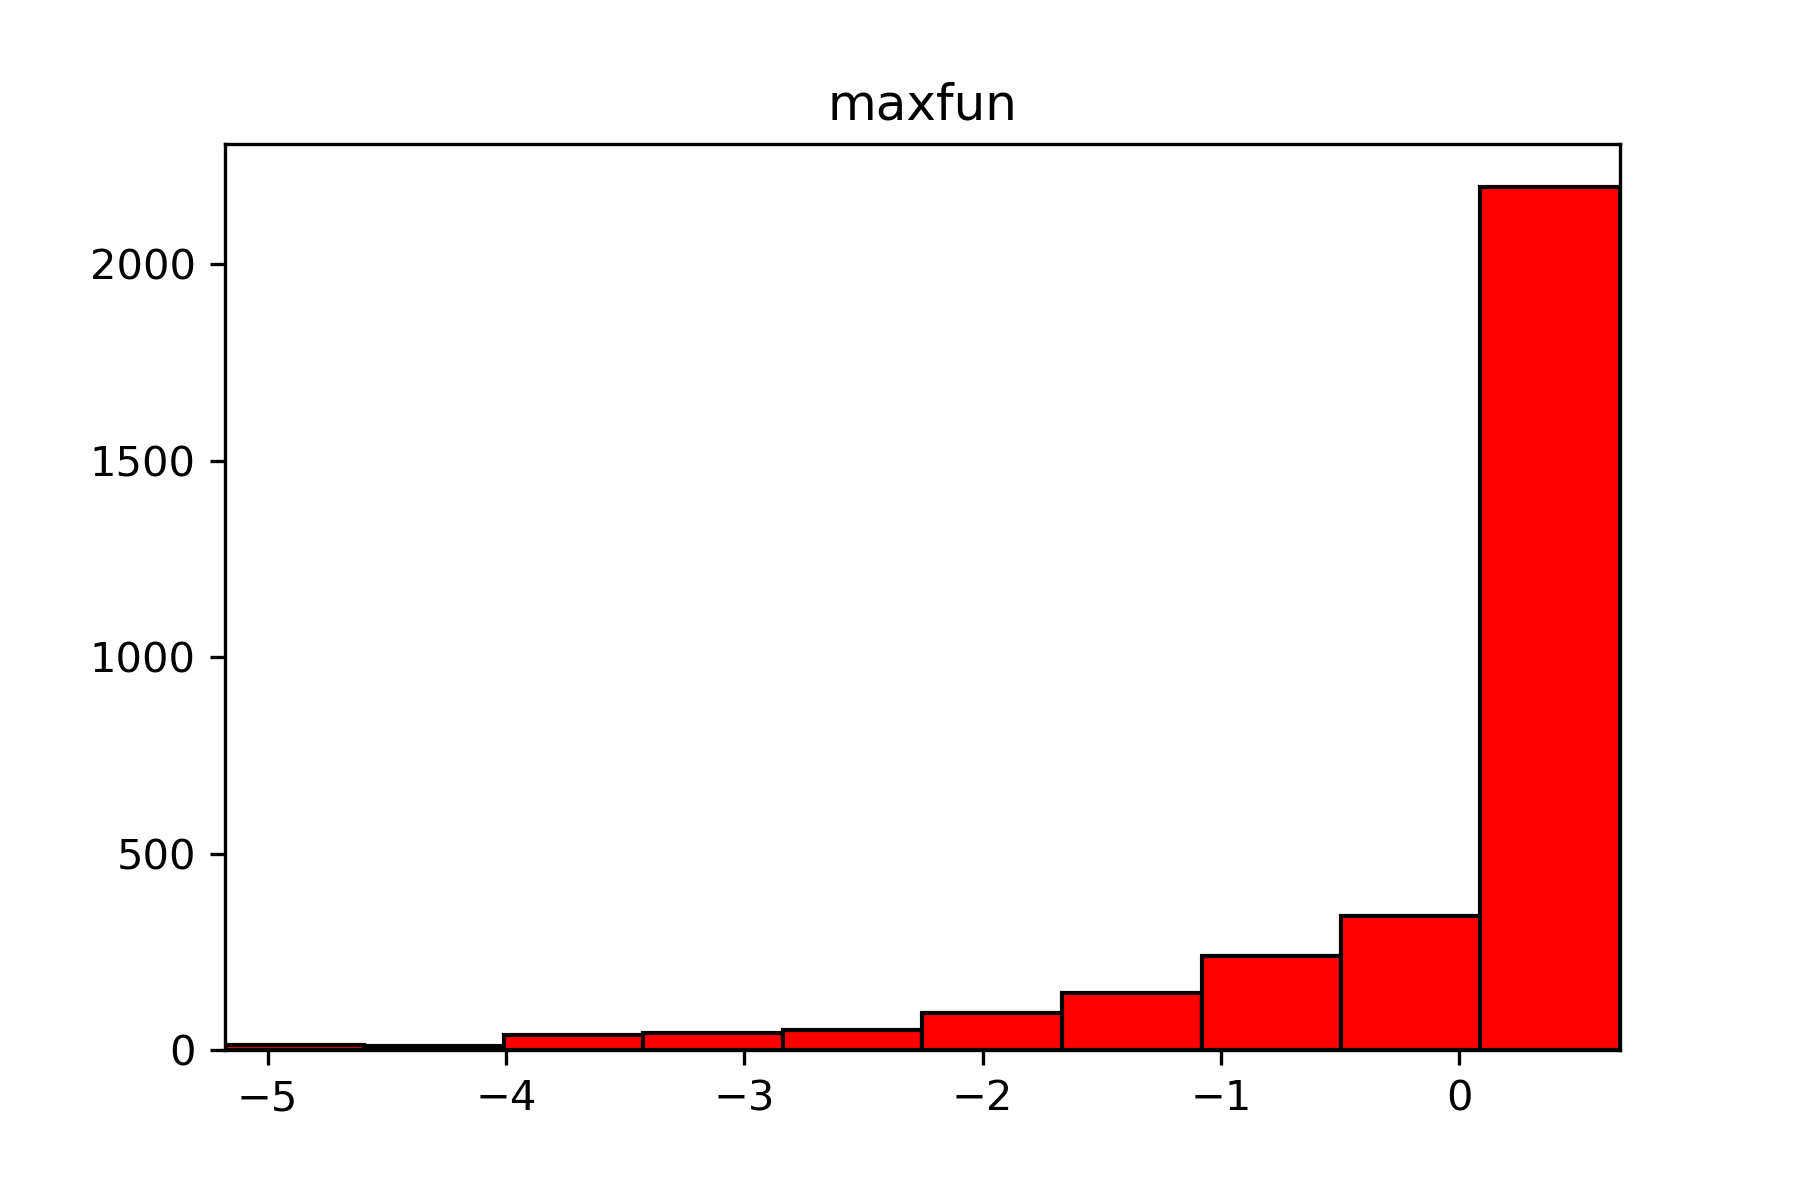
\includegraphics[width=3.85cm]{std_13_maxfun}
        \caption{maxfun}
        \label{fig:sub_std_14}
    \end{subfigure}\hfill
    % meandom
    \begin{subfigure}{0.32\textwidth}
        \centering
        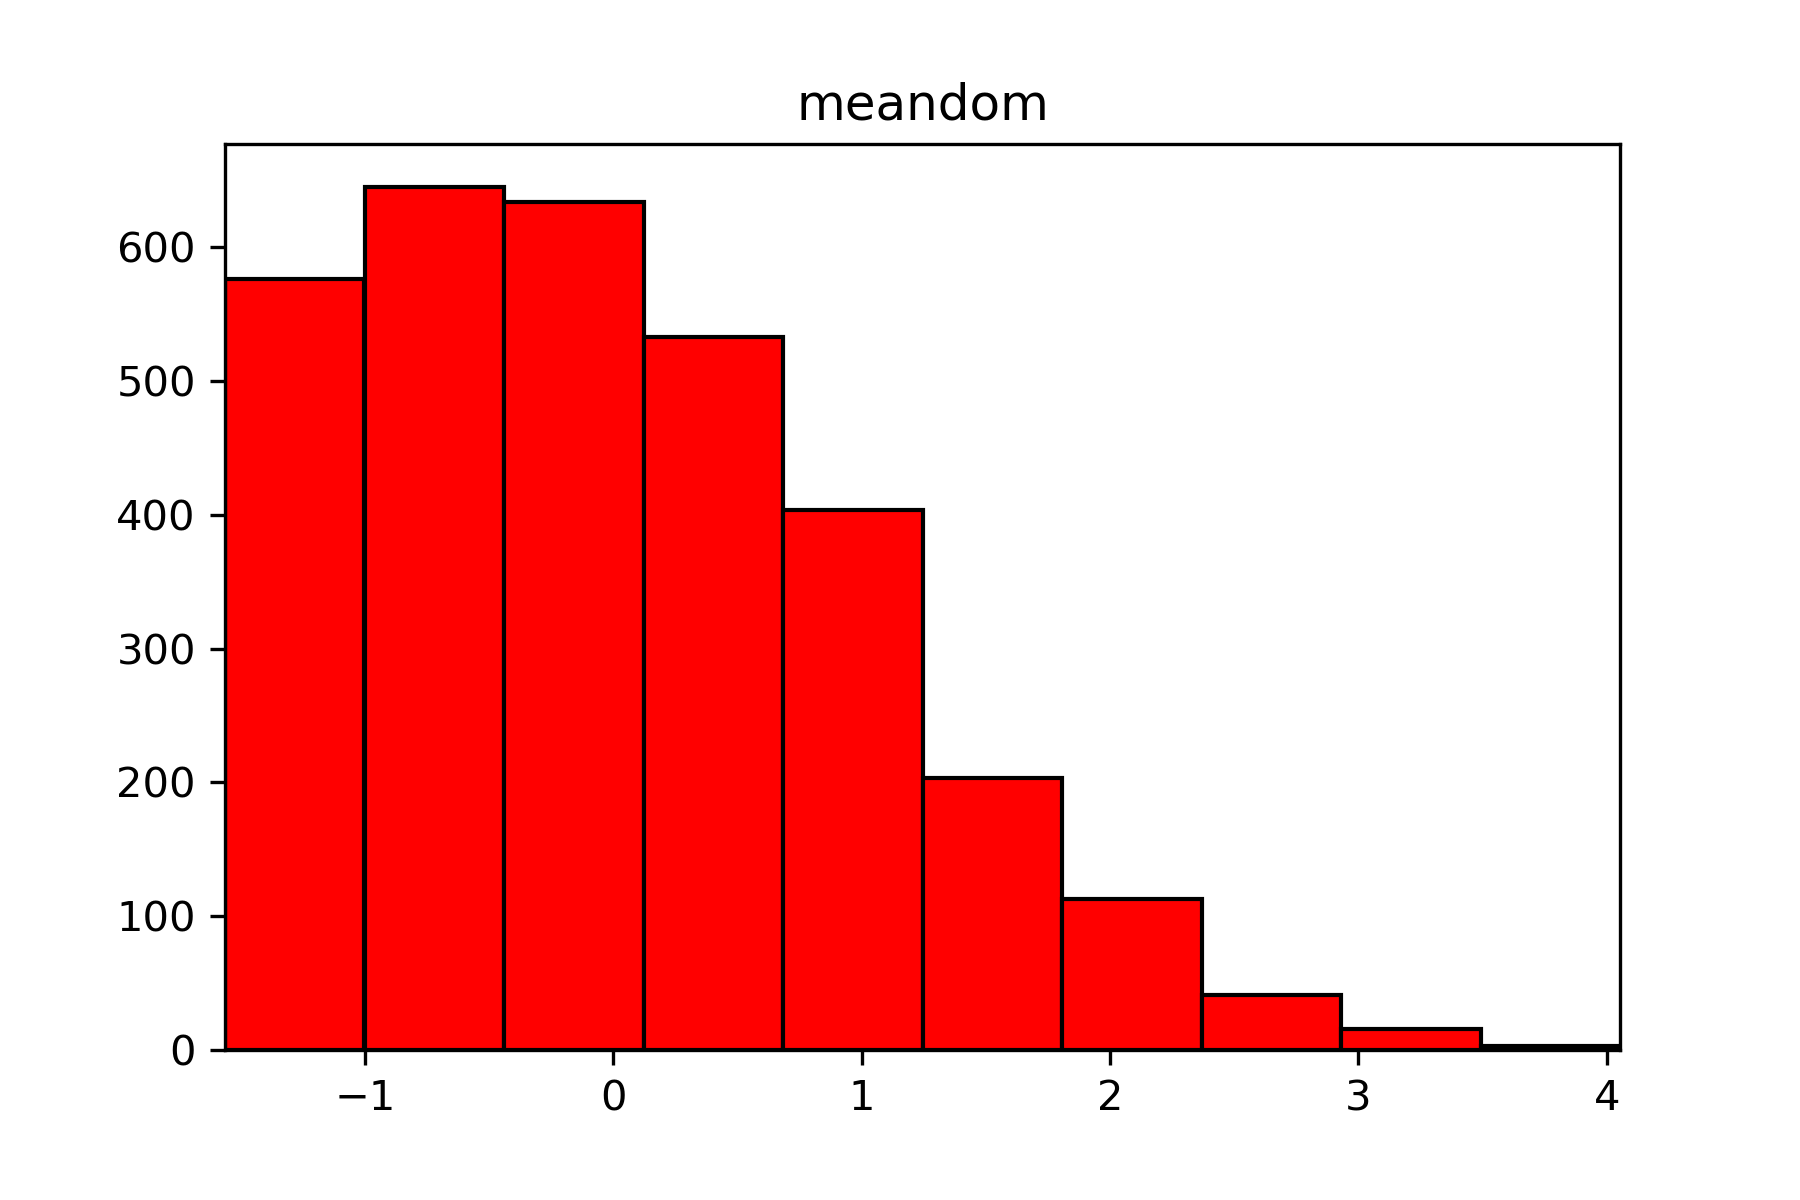
\includegraphics[width=3.85cm]{std_14_meandom}
        \caption{meandom}
        \label{fig:sub_std_15}
    \end{subfigure}\hfill
    % mindom
    \begin{subfigure}{0.32\textwidth}
        \centering
        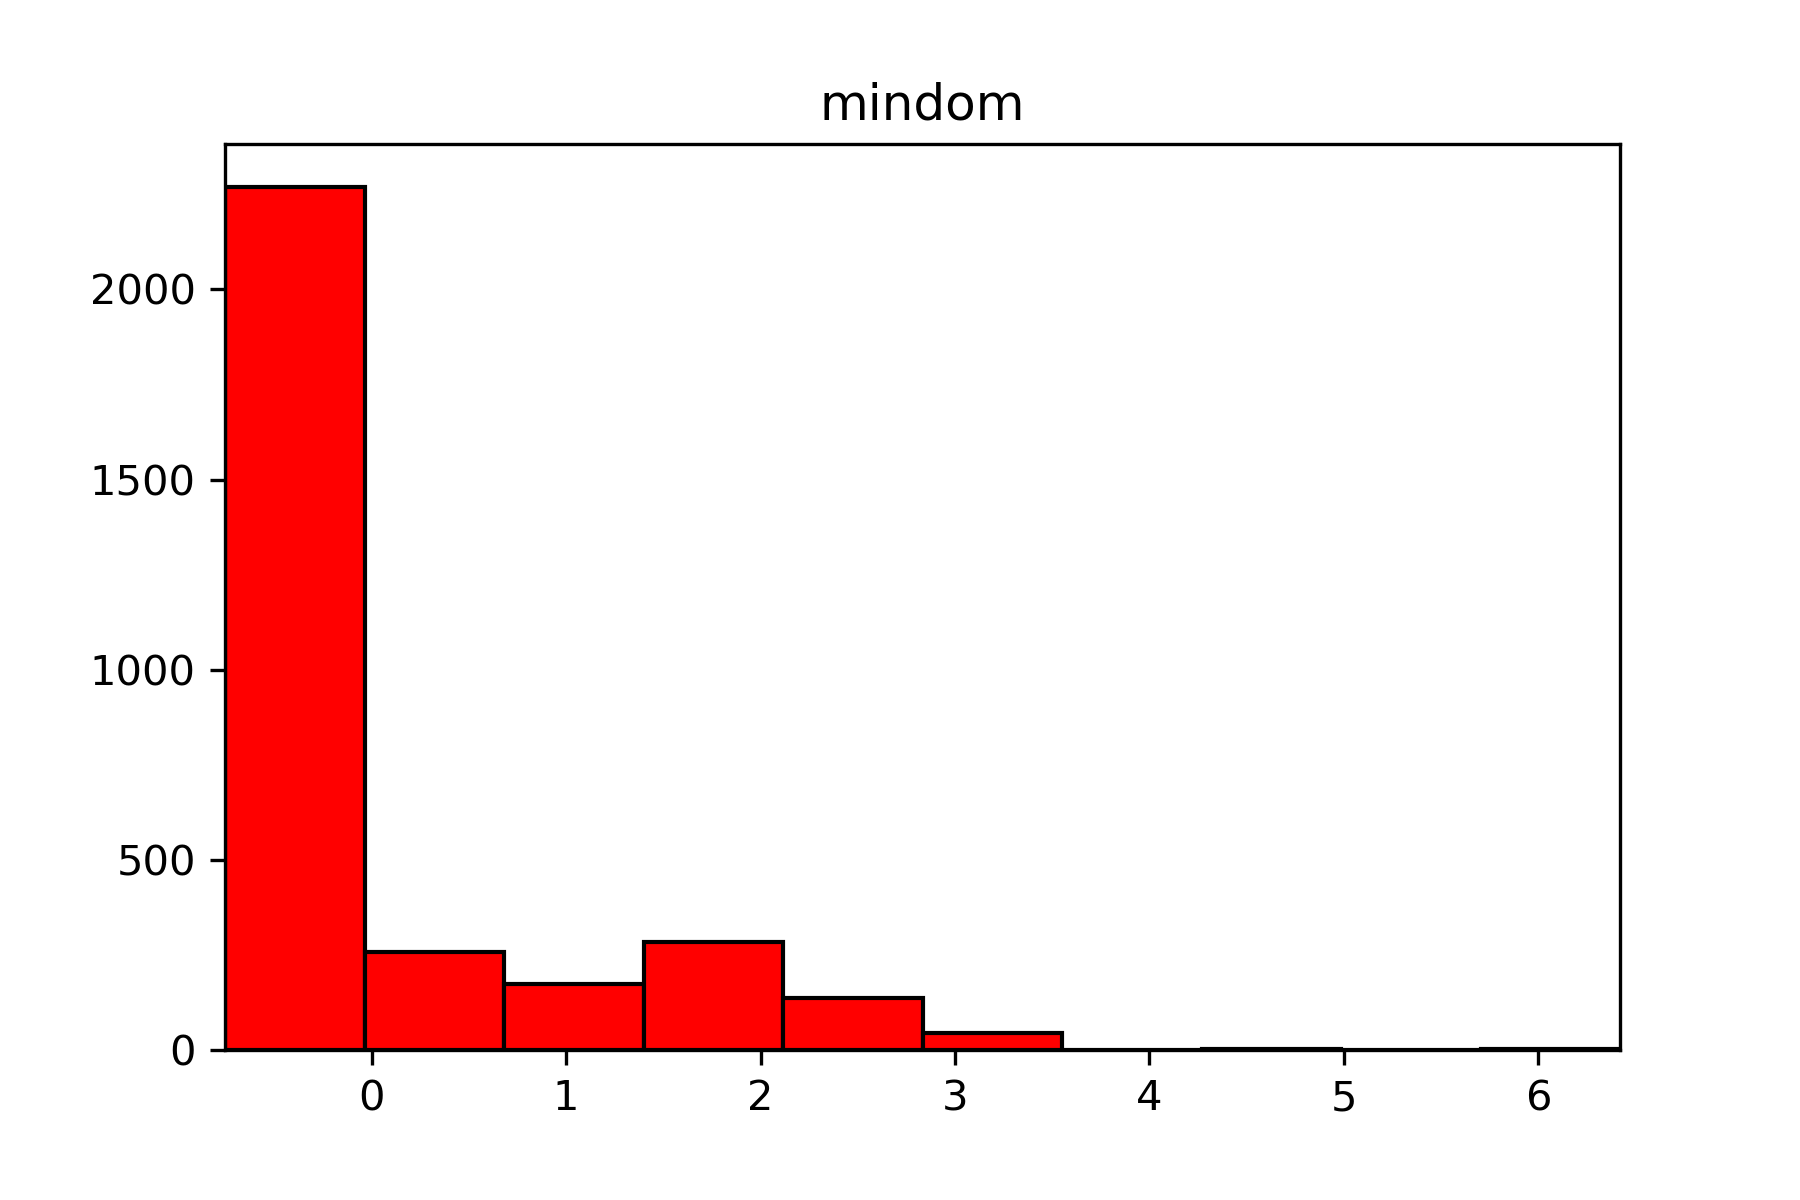
\includegraphics[width=3.85cm]{std_15_mindom}
        \caption{mindom}
        \label{fig:sub_std_16}
    \end{subfigure}\hfill
    % maxdom
    \begin{subfigure}{0.32\textwidth}
        \centering
        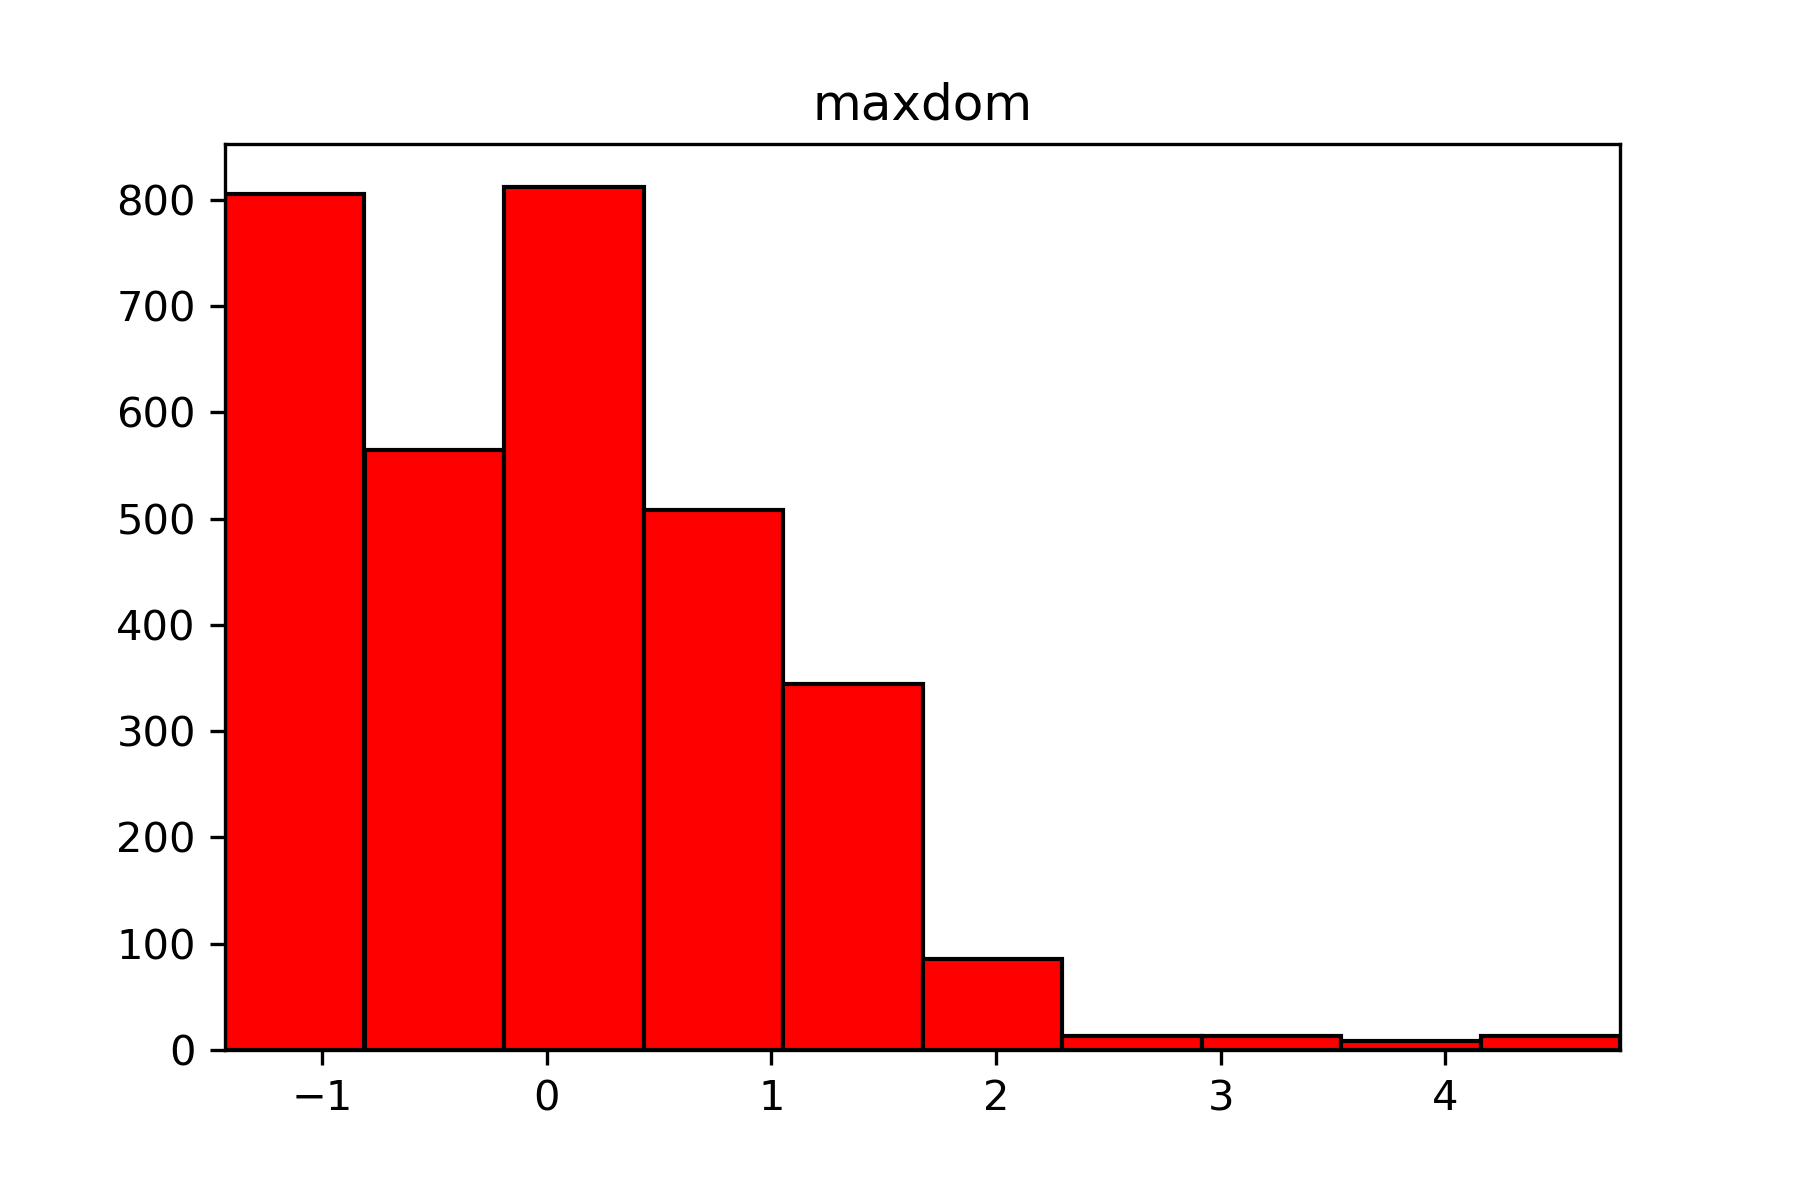
\includegraphics[width=3.85cm]{std_16_maxdom}
        \caption{maxdom}
        \label{fig:sub_std_17}
    \end{subfigure}\hfill
    % dfrange
    \begin{subfigure}{0.32\textwidth}
        \centering
        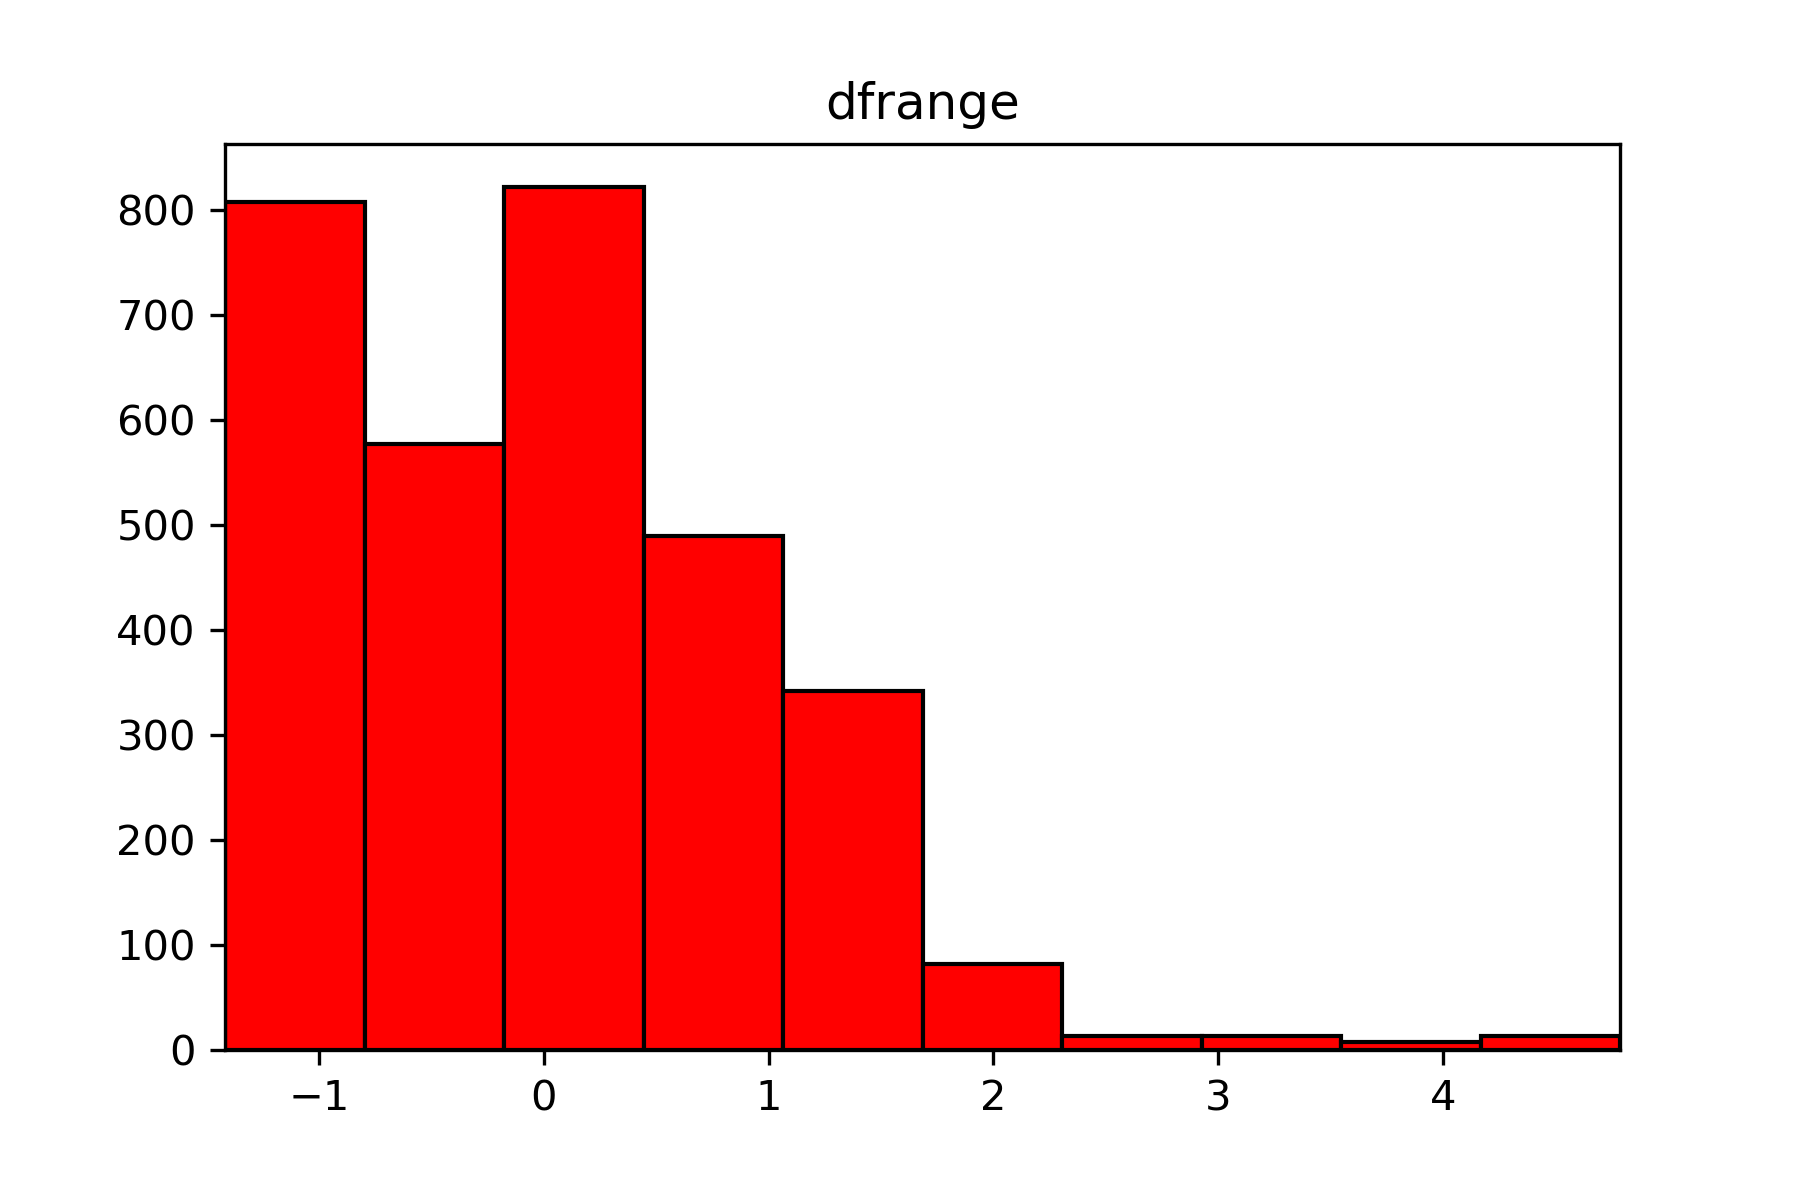
\includegraphics[width=3.85cm]{std_17_dfrange}
        \caption{dfrange}
        \label{fig:sub_std_18}
    \end{subfigure}\hfill
    % modindx
    \begin{subfigure}{0.32\textwidth}
        \centering
        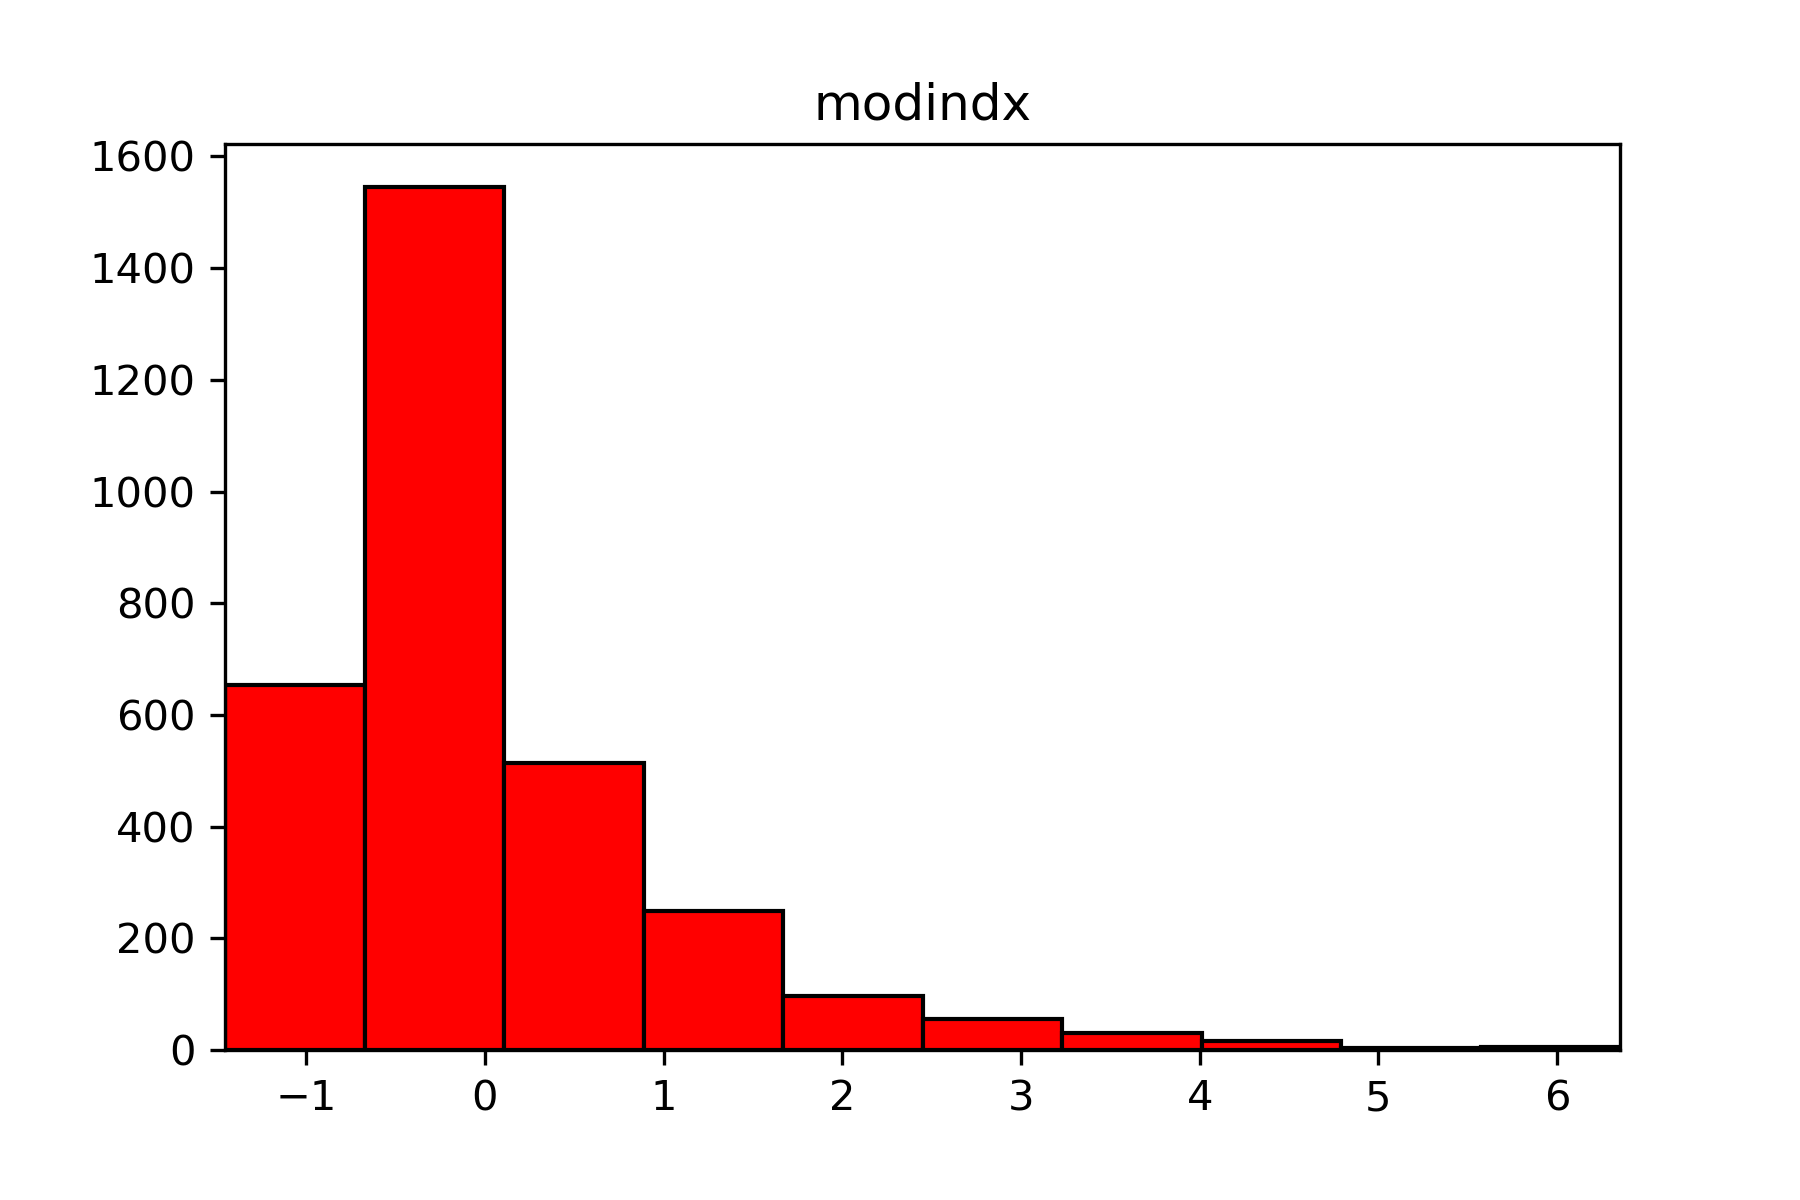
\includegraphics[width=3.85cm]{std_18_modindx}
        \caption{modindx}
        \label{fig:sub_std_19}
    \end{subfigure}
    % caption and label
    \caption{Histograms of input features after data standardization}
    \label{fig:pre-ex1-std_histograms}
\end{figure}



\begin{figure}[H]
    \centering
    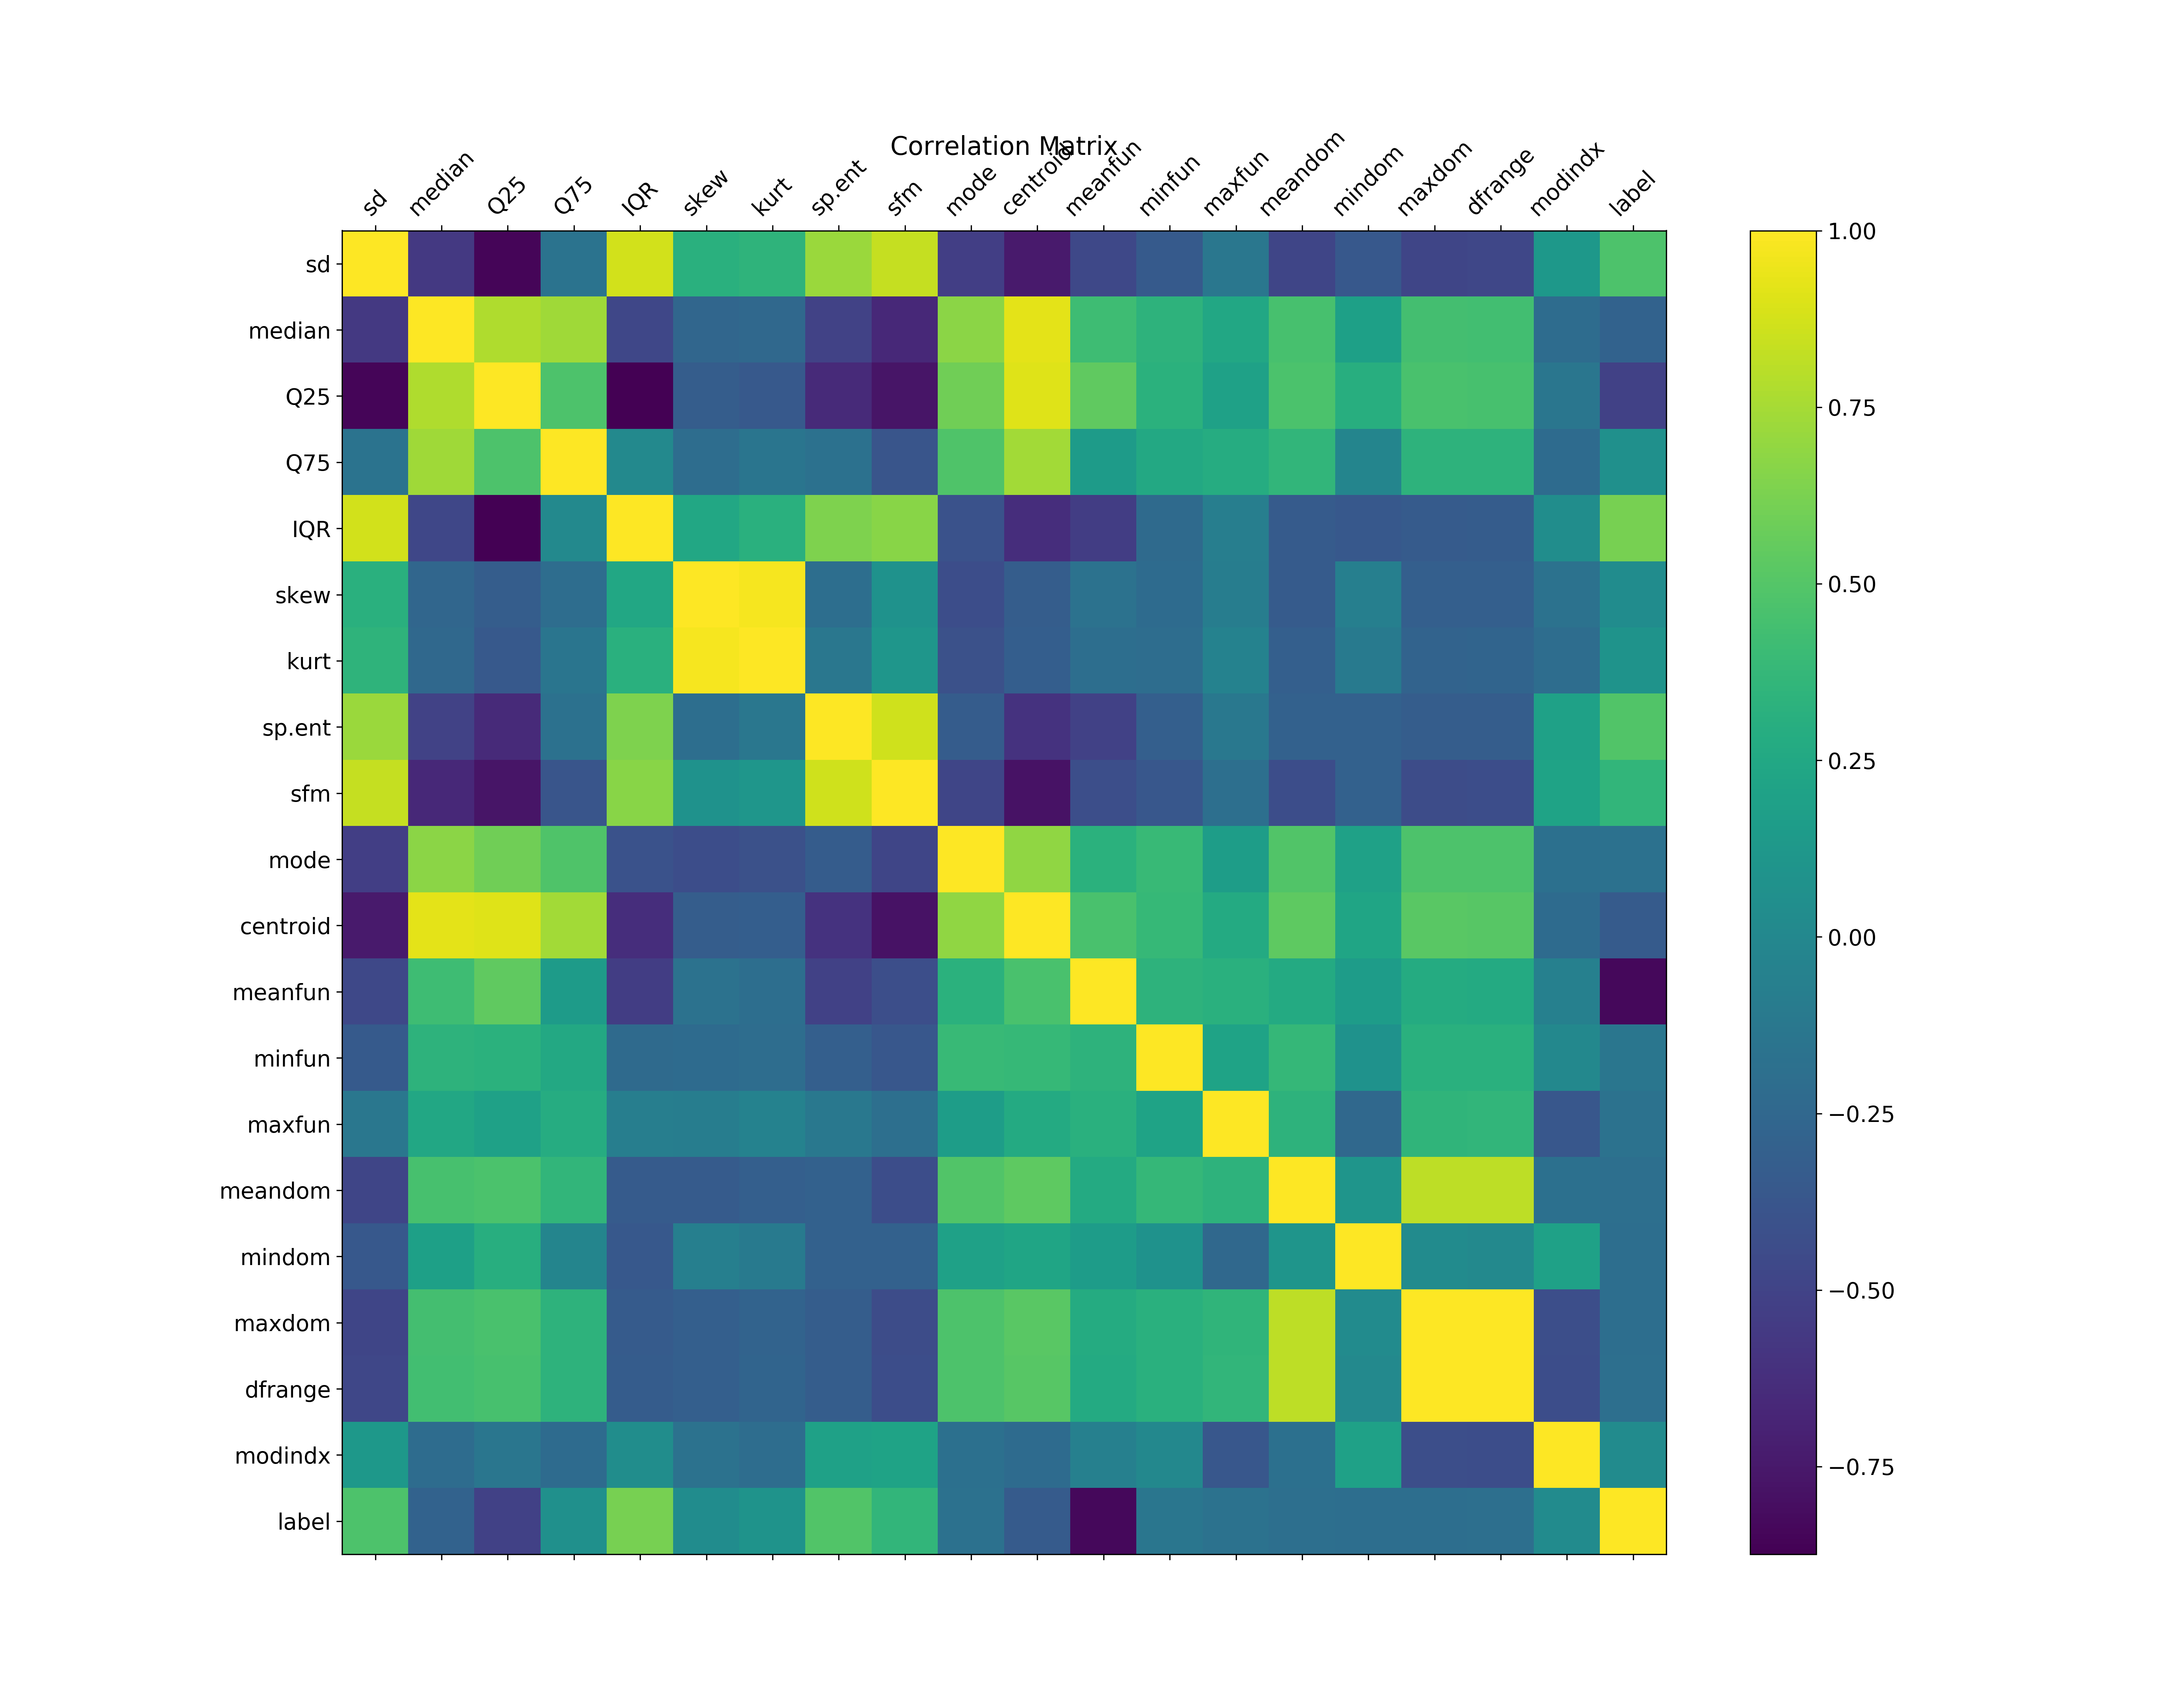
\includegraphics[width=12cm]{correlation}
    \caption{Correlation between input features}
    \label{fig:pre-ex1-correlation}
\end{figure}

\begin{figure}[H]
    \centering
    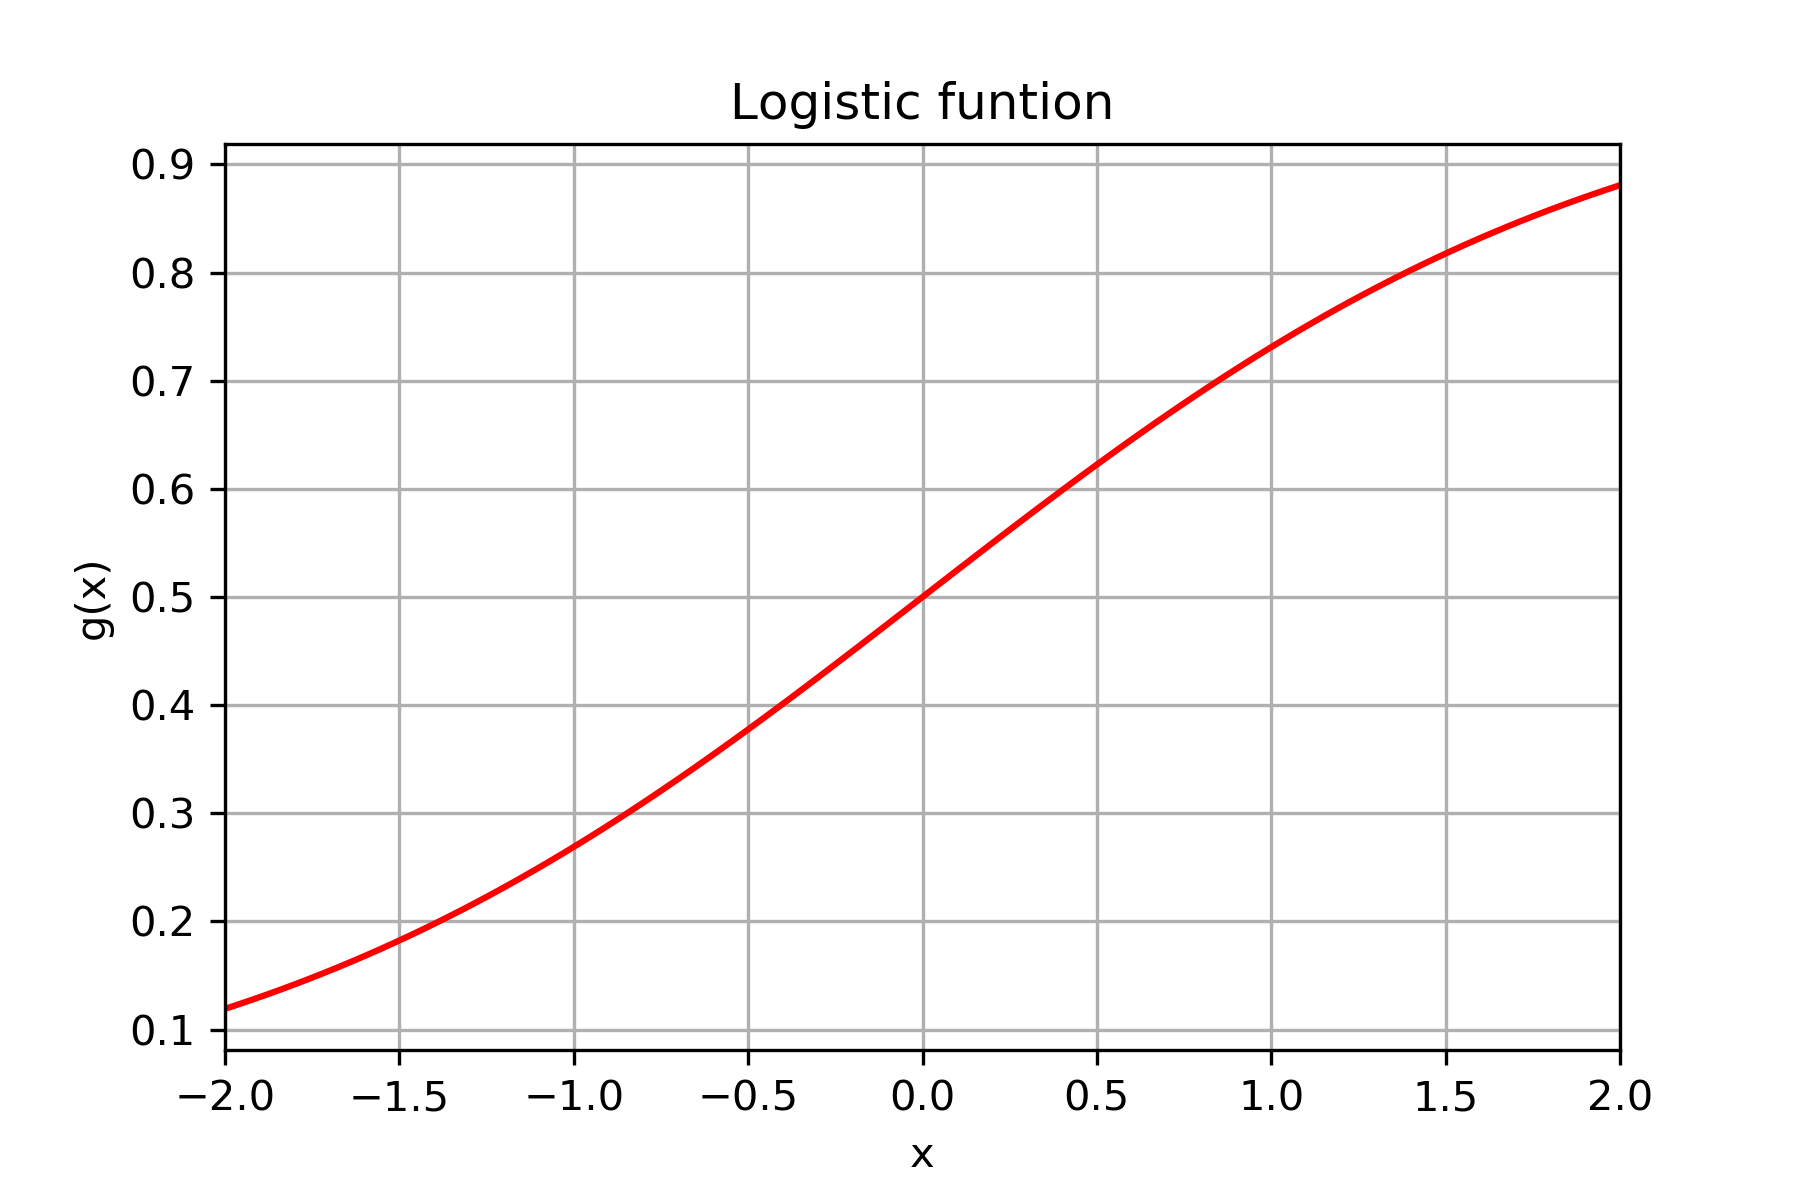
\includegraphics[width=12cm]{logistic_function}
    \caption{Logistic function}
    \label{fig:pre-ex1-logistic}
\end{figure}

\begin{figure}[H]
    \centering
    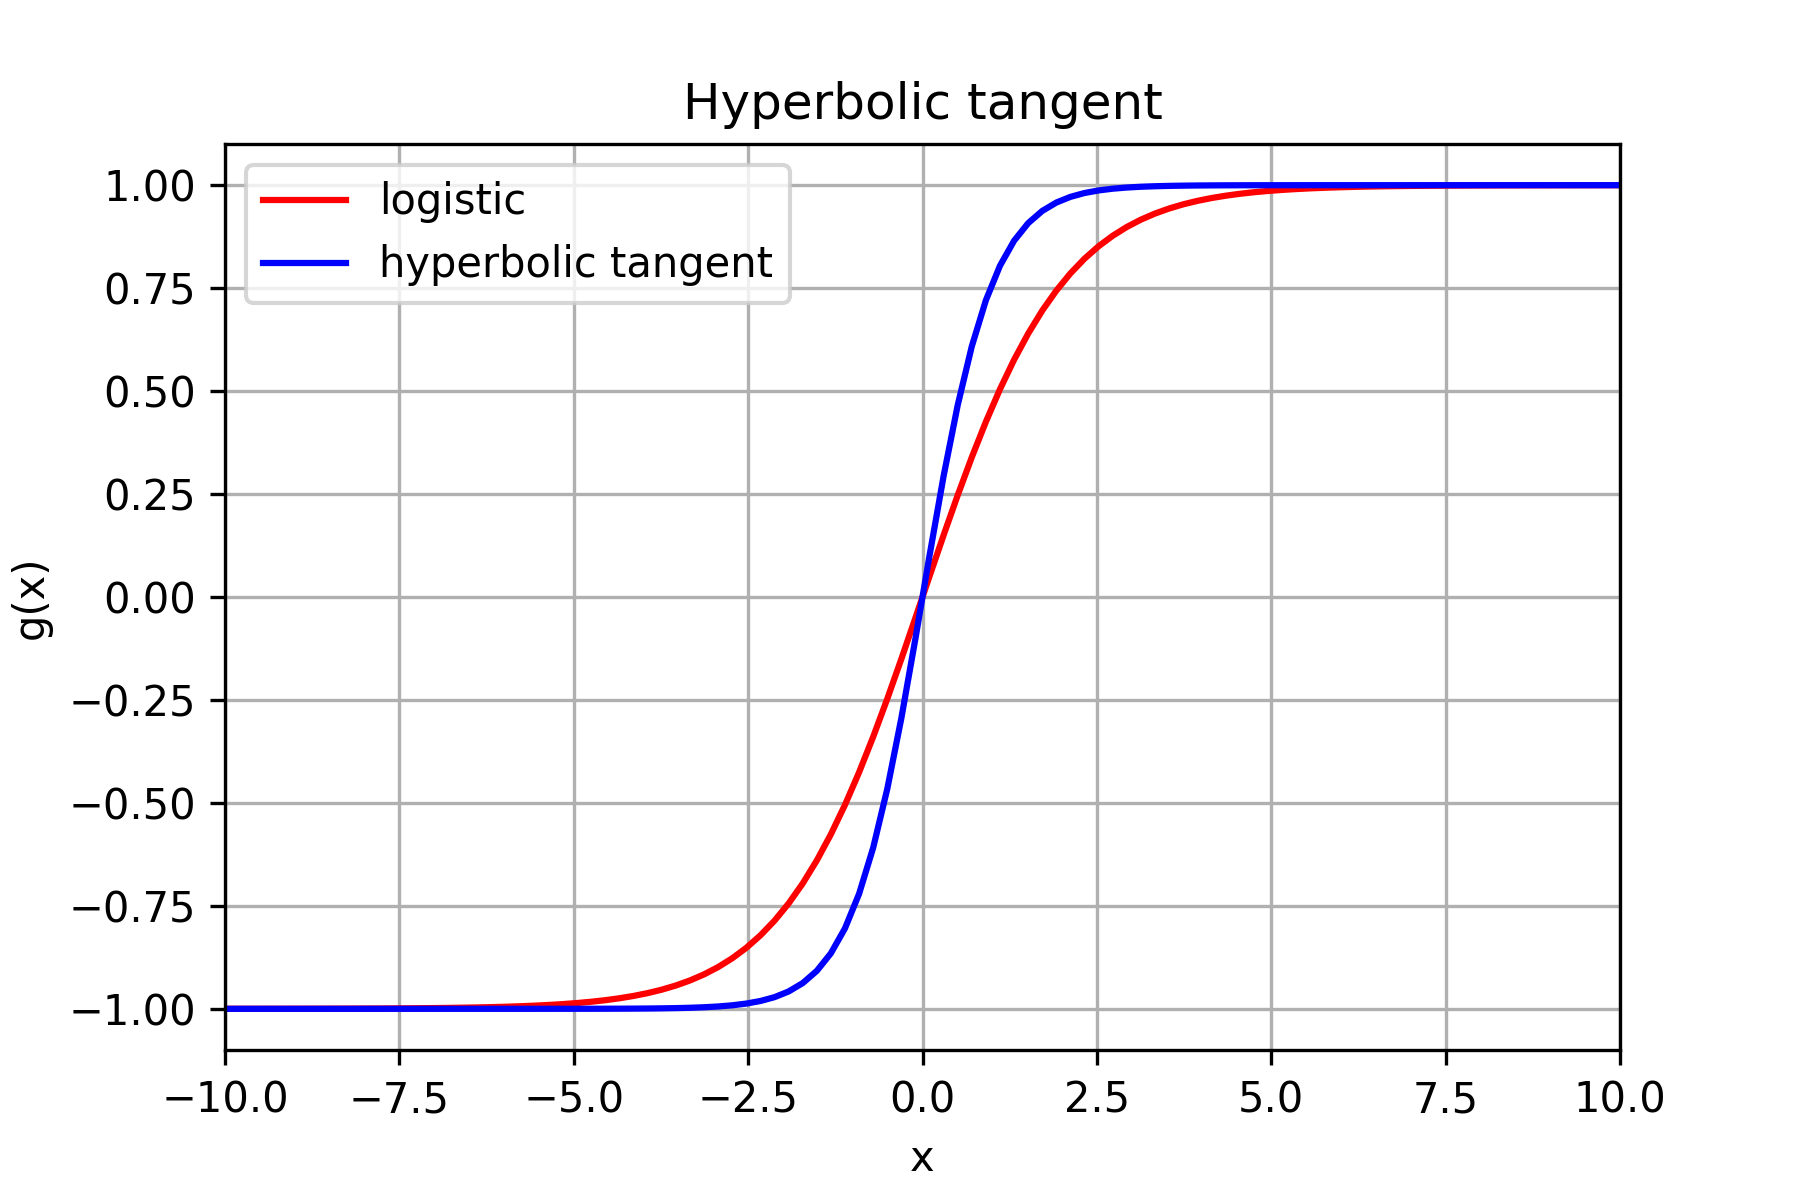
\includegraphics[width=12cm]{logistic_vs_tanh}
    \caption{Comparasion between hyperbolic tangent and logistic function(scaled and with offset)}
    \label{fig:pre-ex1-logistic_tanh}
\end{figure}

%=======================================
\subsection{b) }
%=======================================

\begin{figure}[H]
    \centering
    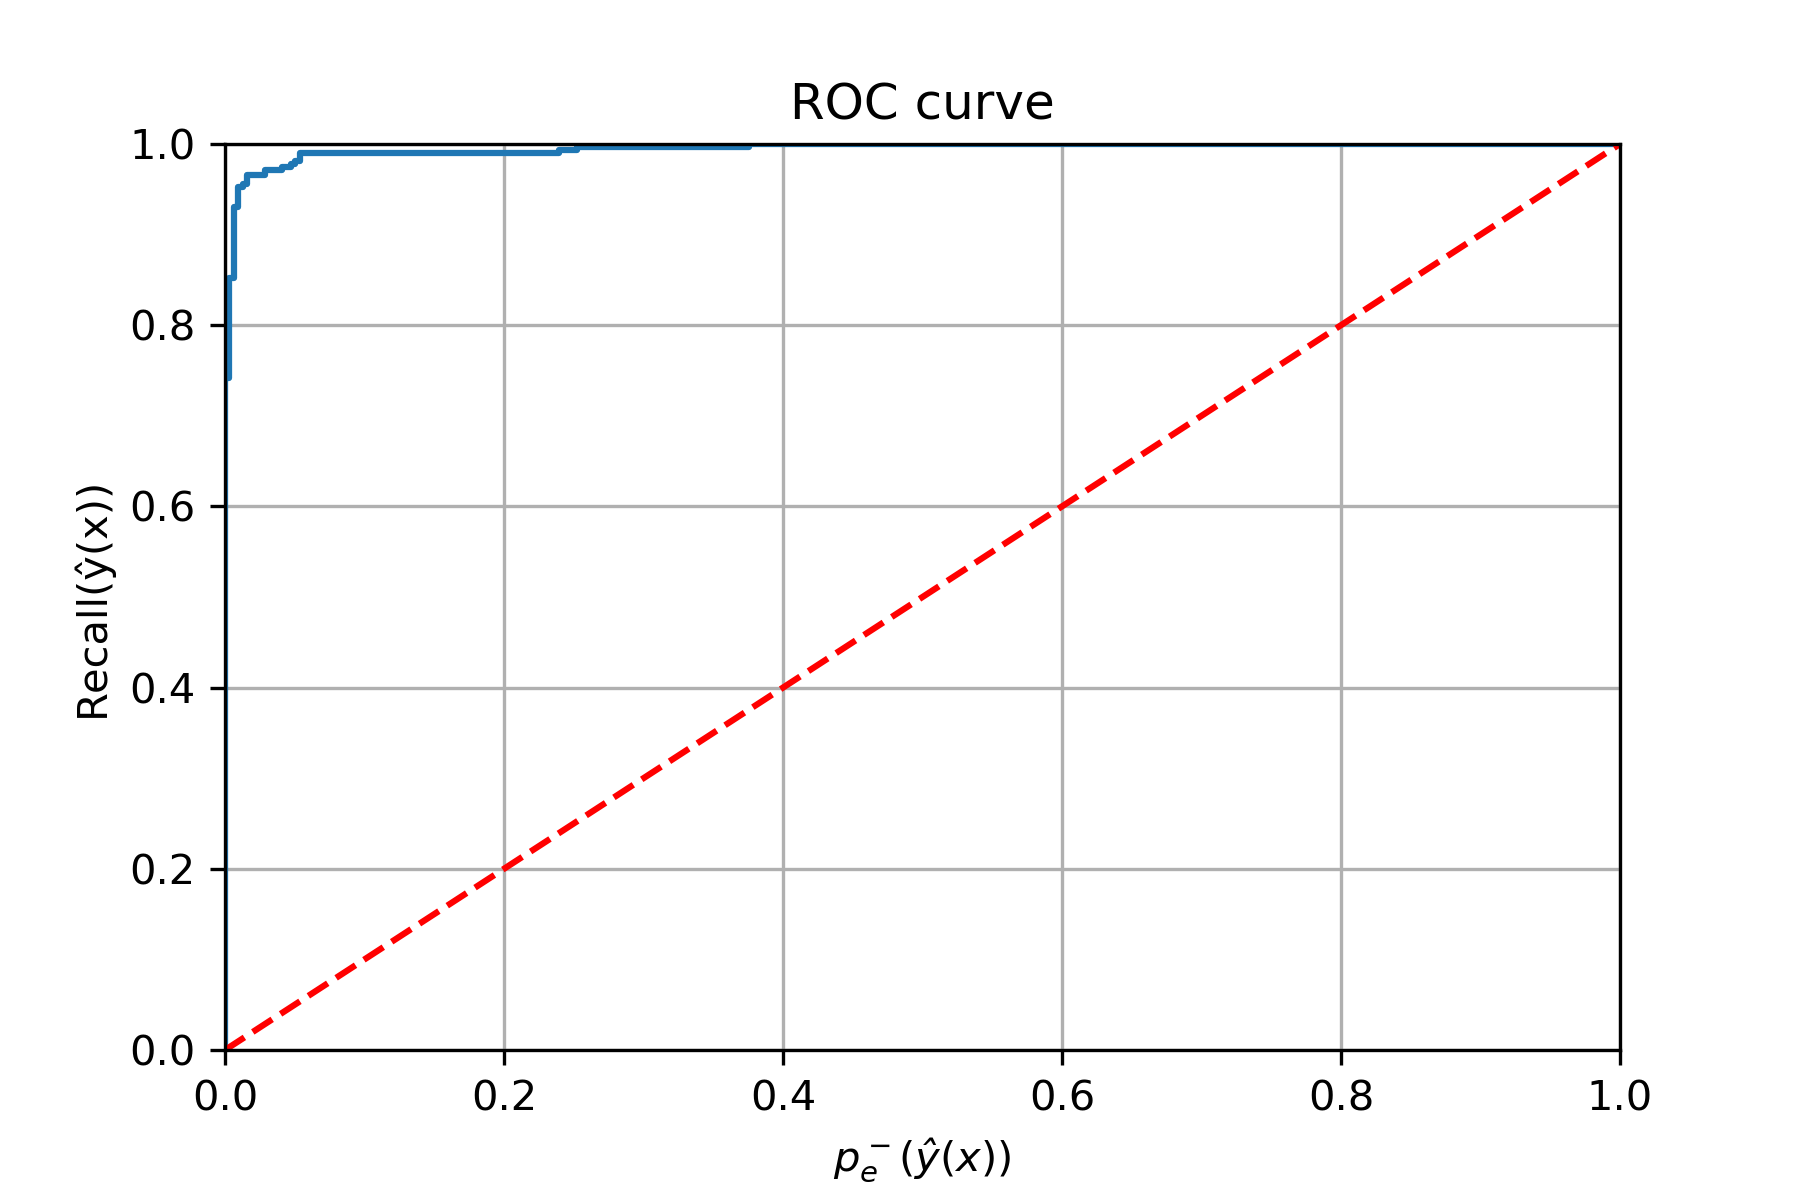
\includegraphics[width=12cm]{ROC}
    \caption{ROC curve}
    \label{fig:ex1-roc}
\end{figure}

\begin{figure}[H]
    \centering
    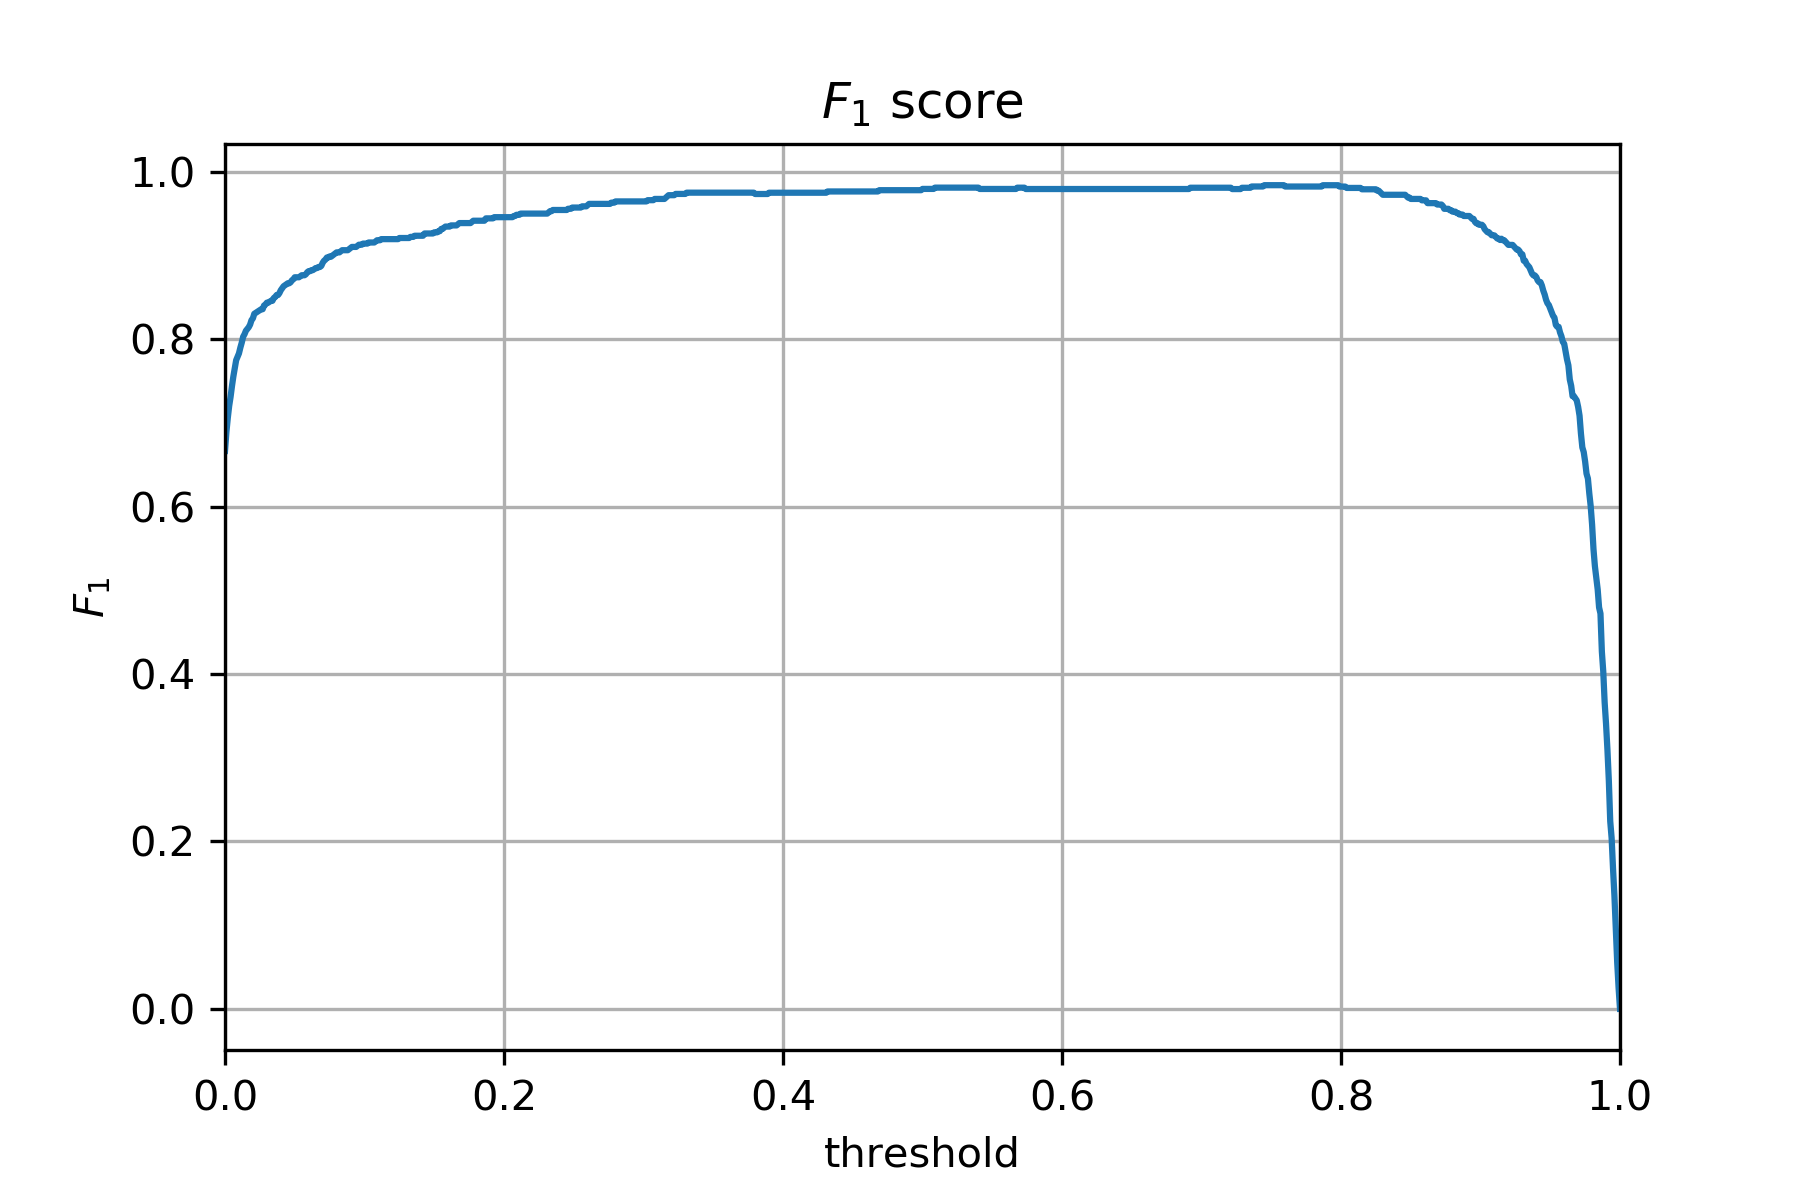
\includegraphics[width=12cm]{F1_score}
    \caption{F1-score curve}
    \label{fig:ex1-f1_score}
\end{figure}

\begin{figure}[H]
    \centering
    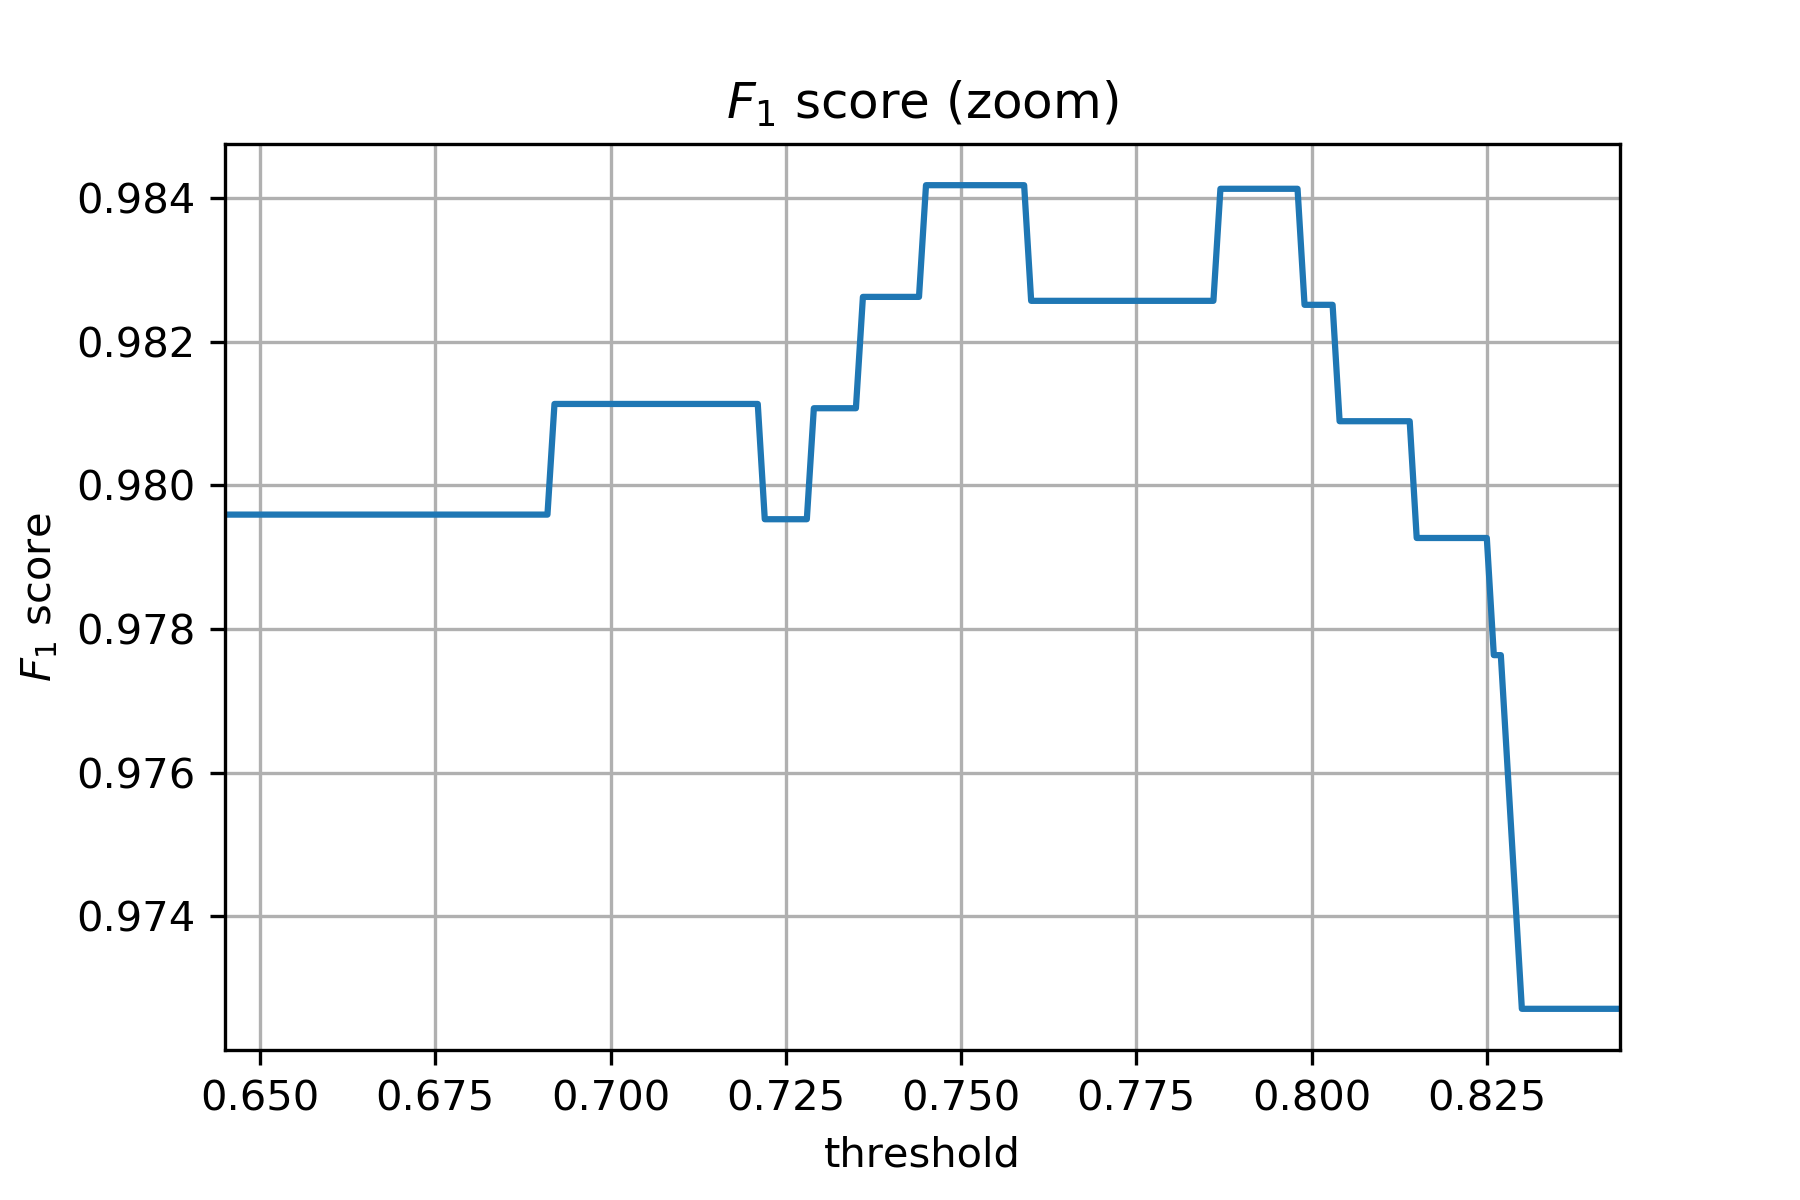
\includegraphics[width=12cm]{F1_score_zoom}
    \caption{Zoom in F1-score curve}
    \label{fig:ex1-f1_score_zoom}
\end{figure}

%=======================================
\subsection{c) }
%=======================================

\paragraph{}

%=================================================
\section{Part 2 - Multiclass Classification}
%=================================================

%=======================================
\subsection{a) }
%=======================================

**output** <br>
1 – caminhada <br>
2 – subindo escadas <br>
3 – descendo escadas <br>
4 – sentado <br>
5 – em pé <br>
6 – deitado <br>
<br>
**one-hot enconding** <br>
[1 0 0 0 0 0]$^T$: walking <br>
[0 1 0 0 0 0]$^T$: climbing stairs <br>
[0 0 1 0 0 0]$^T$: going down stairs <br>
[0 0 0 1 0 0]$^T$: seated <br>
[0 0 0 0 1 0]$^T$: standing <br>
[0 0 0 0 0 1]$^T$: lying <br>

\begin{figure}[H]
    \centering
    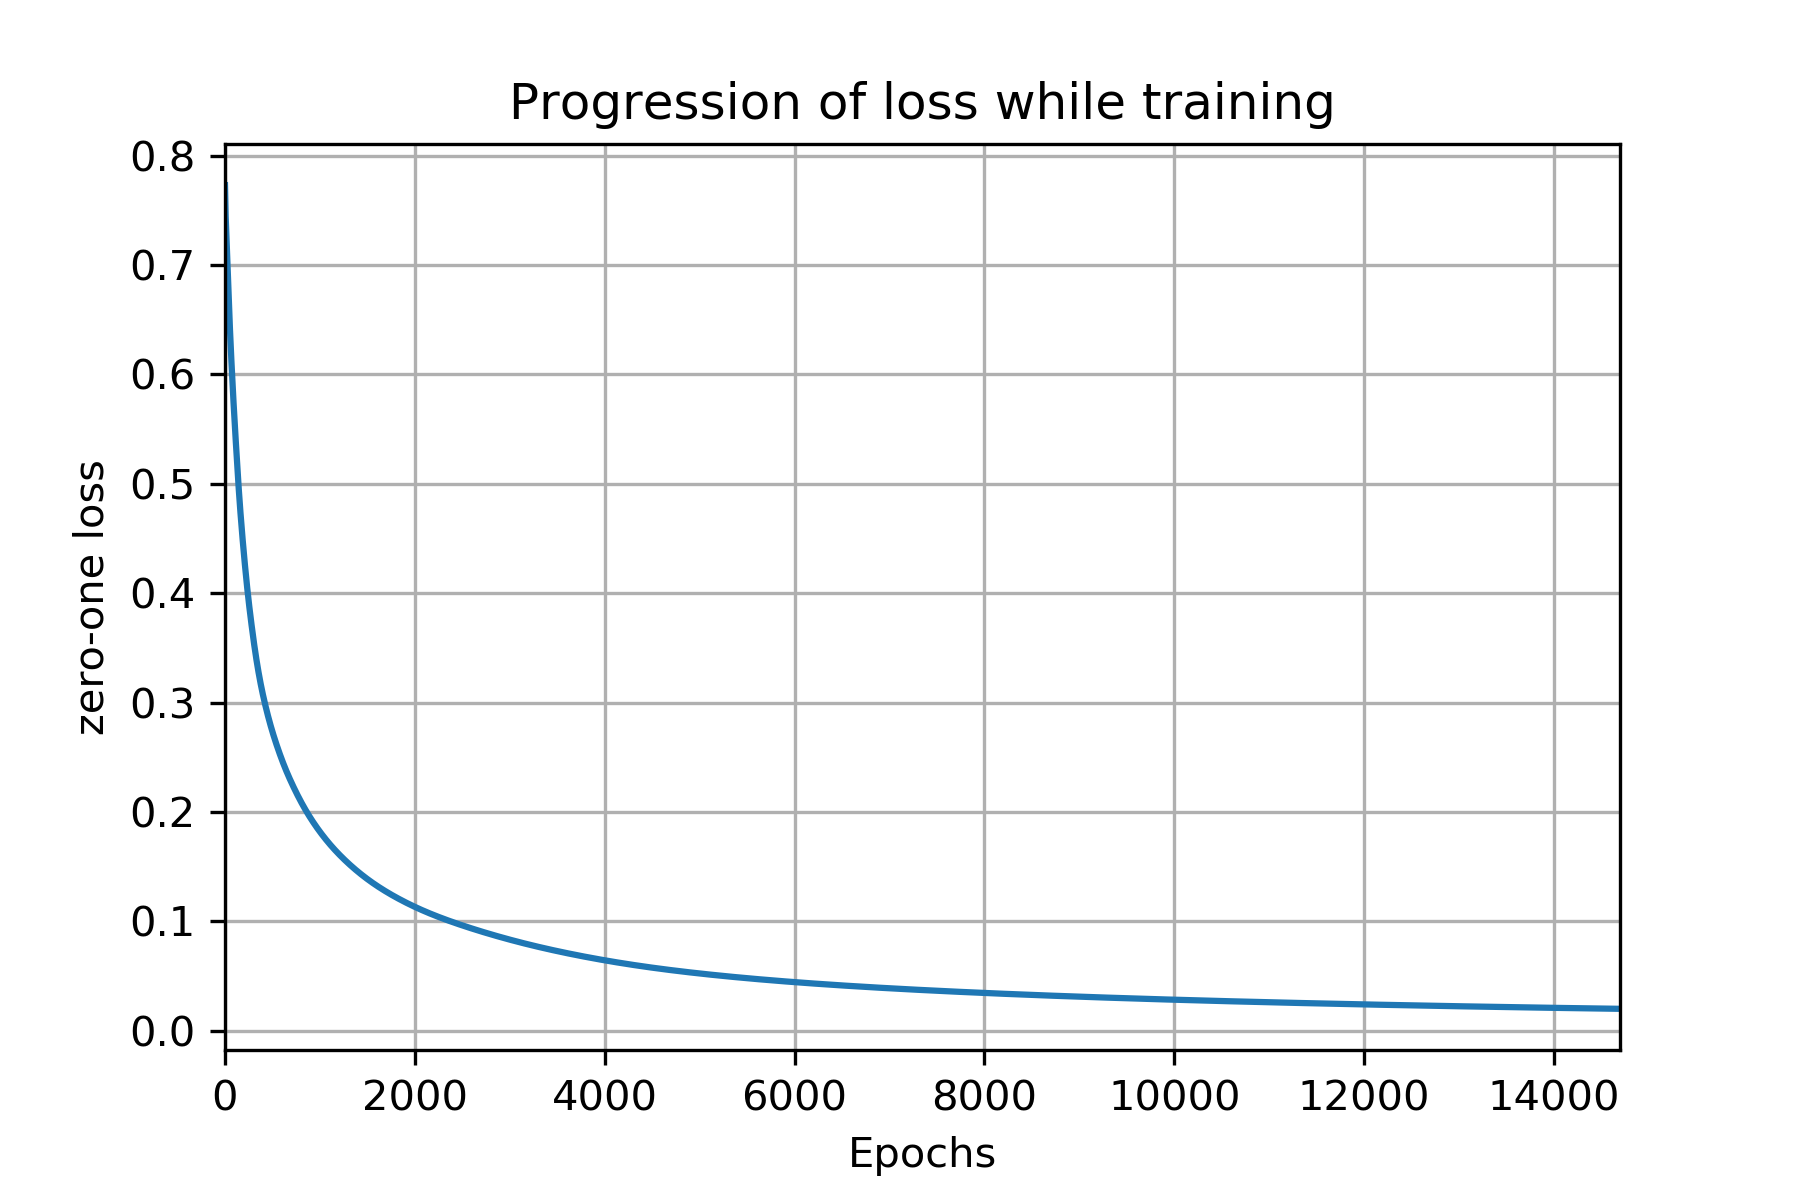
\includegraphics[width=12cm]{zero_one_loss}
    \caption{Zero-one loss curve}
    \label{fig:ex2-a-zero_one_loss}
\end{figure}

\begin{figure}[H]
    \centering
    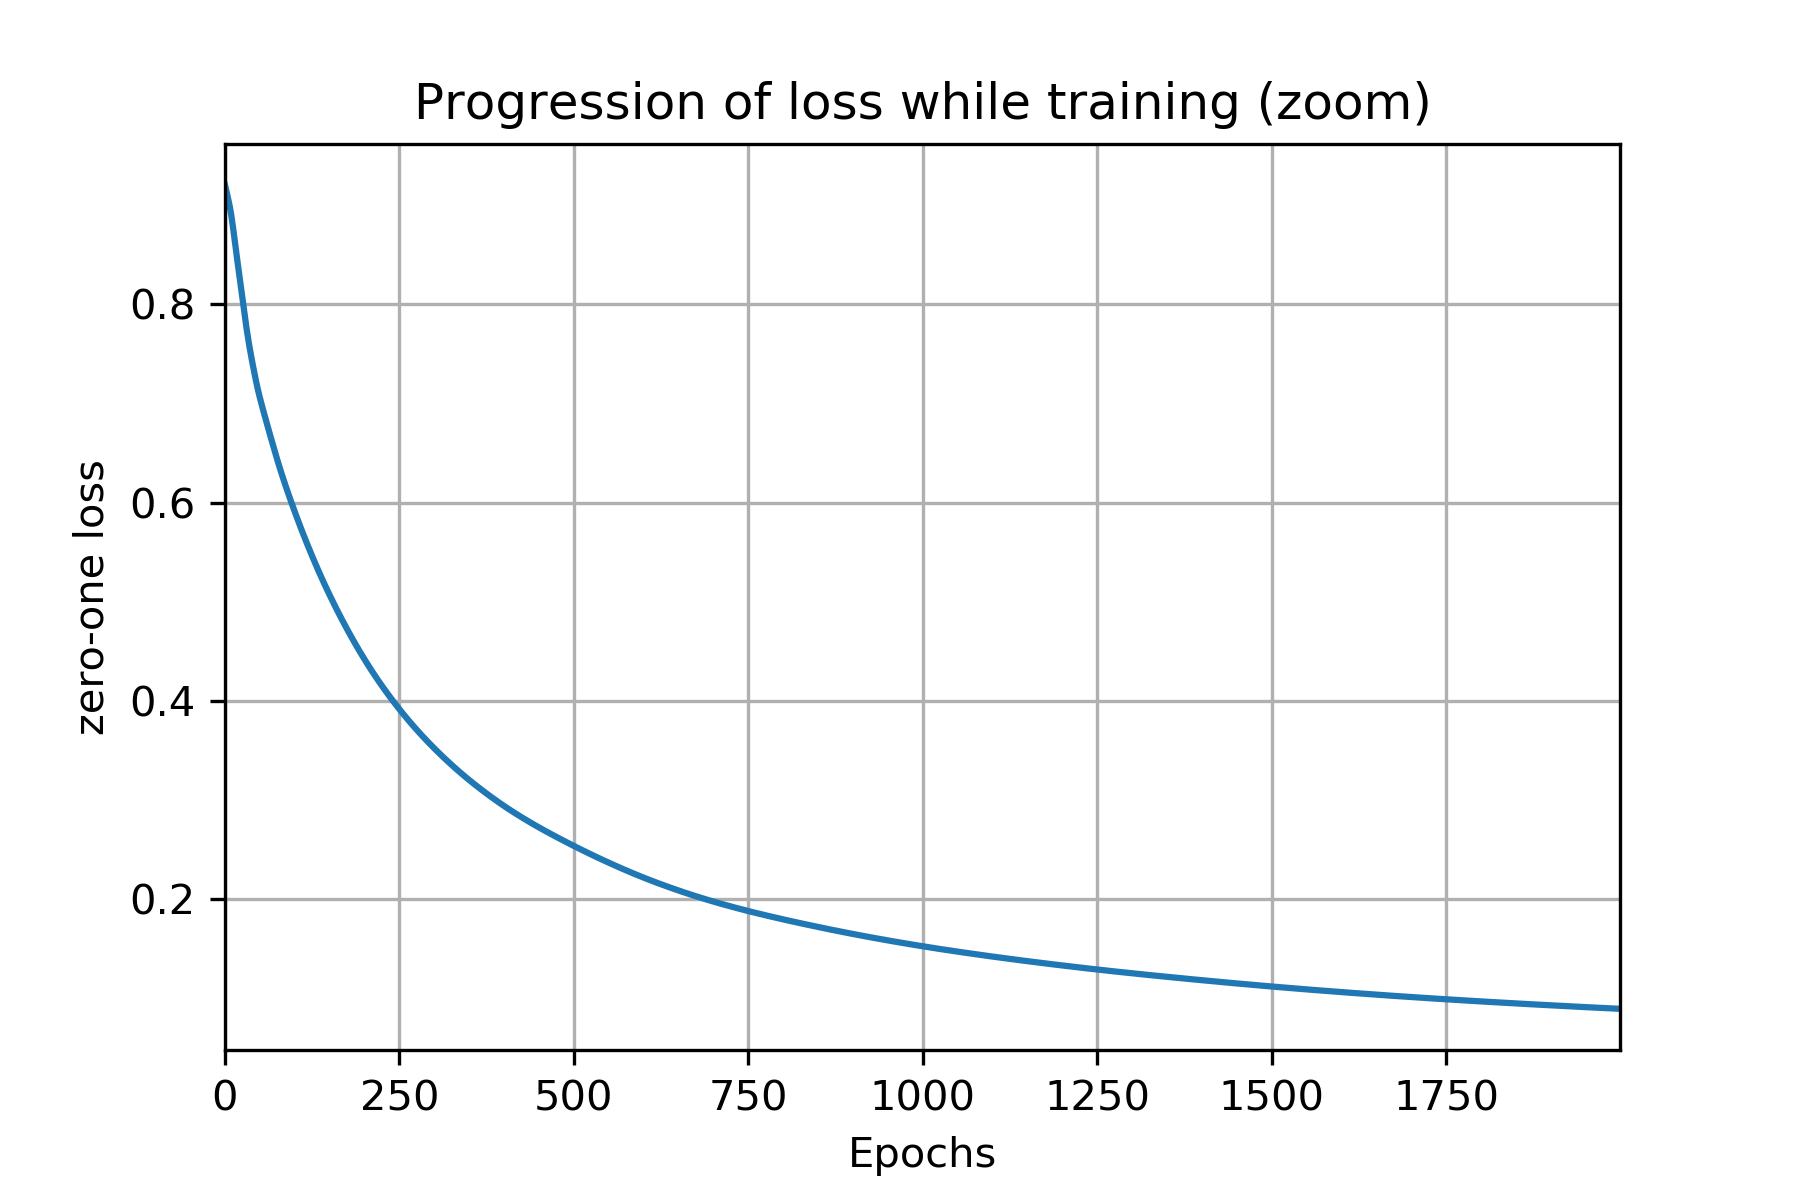
\includegraphics[width=12cm]{zero_one_loss_zoom}
    \caption{Zoom in zero-one loss curve}
    \label{fig:ex2-a-zero_one_loss_zoom}
\end{figure}

%=======================================
\subsection{b) }
%=======================================

\begin{figure}[H]
    \centering
    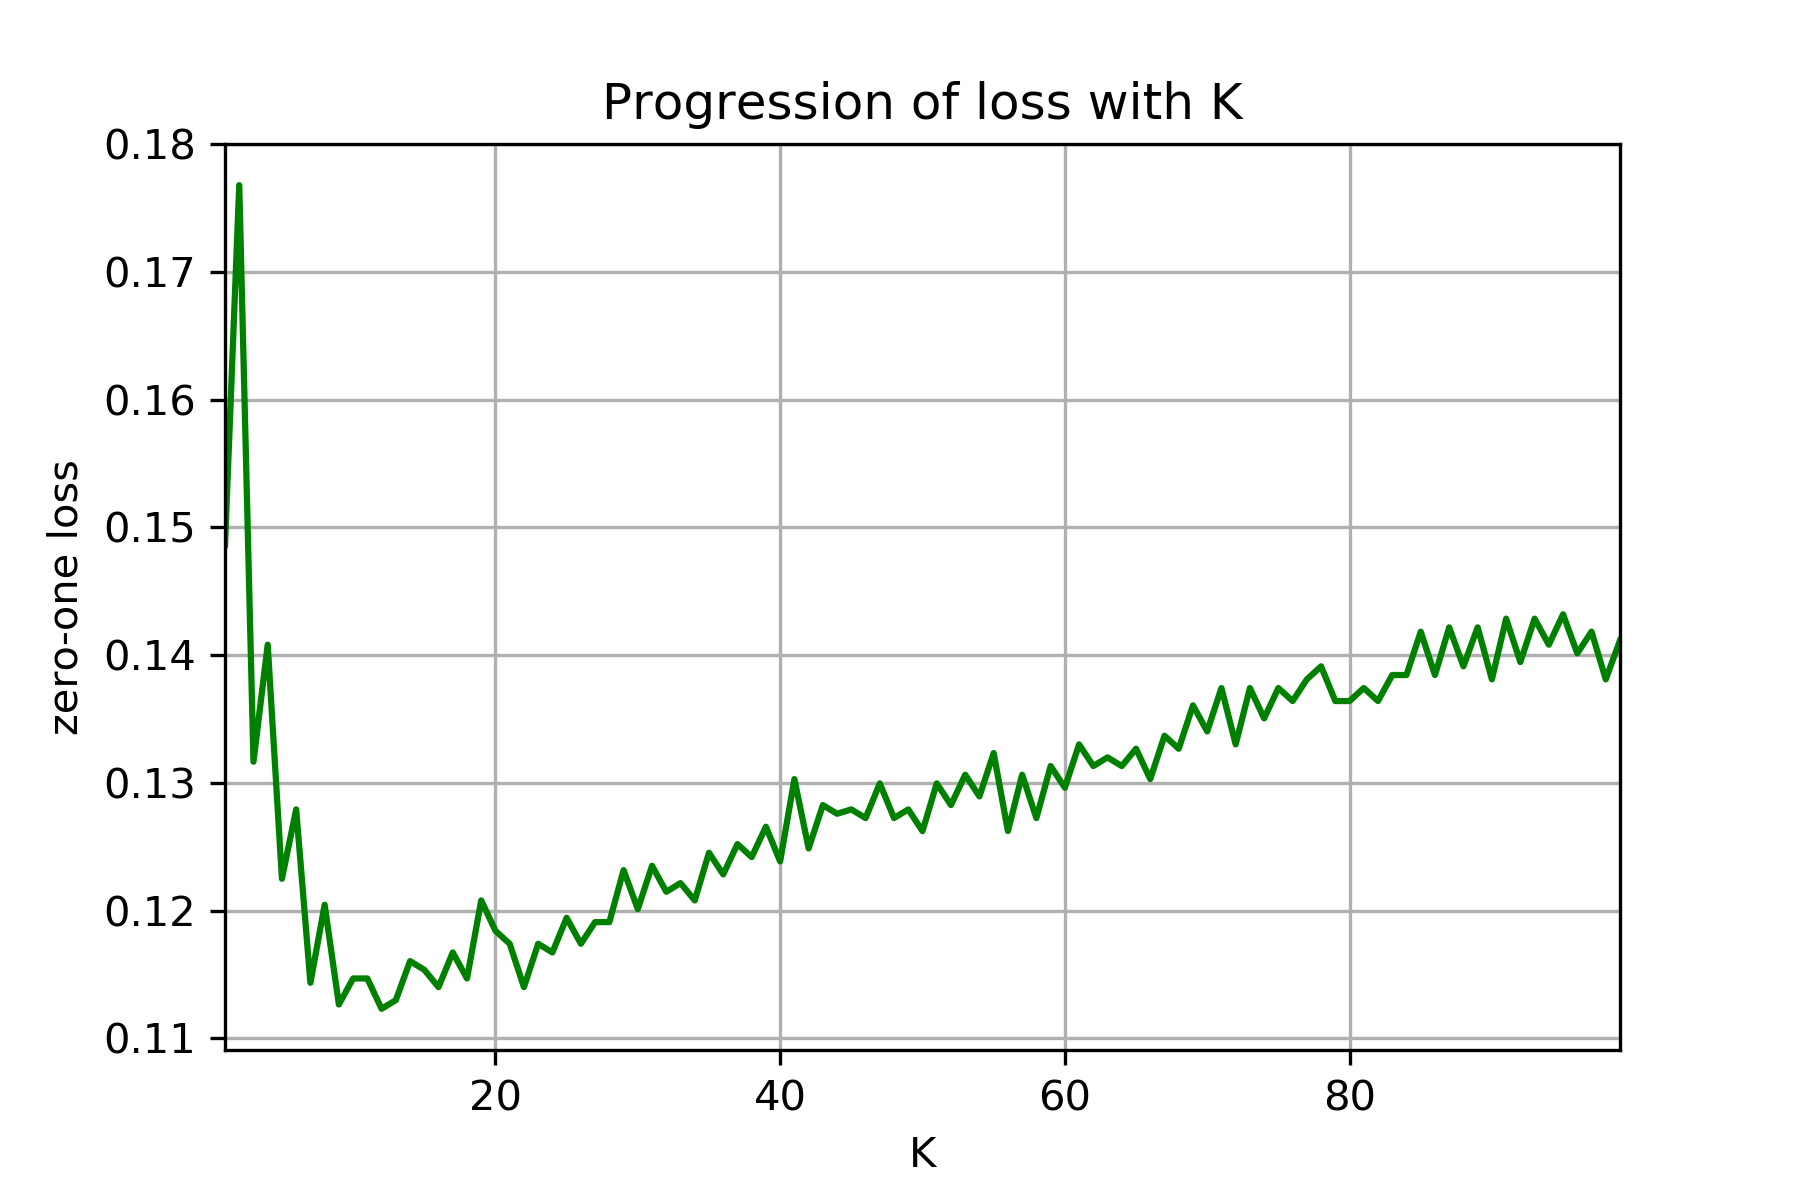
\includegraphics[width=12cm]{error_uniform}
    \caption{Zero-one loss curve (uniform weights}
    \label{fig:ex2-b-error_uniform_0}
\end{figure}

\begin{figure}[H]
    \centering
    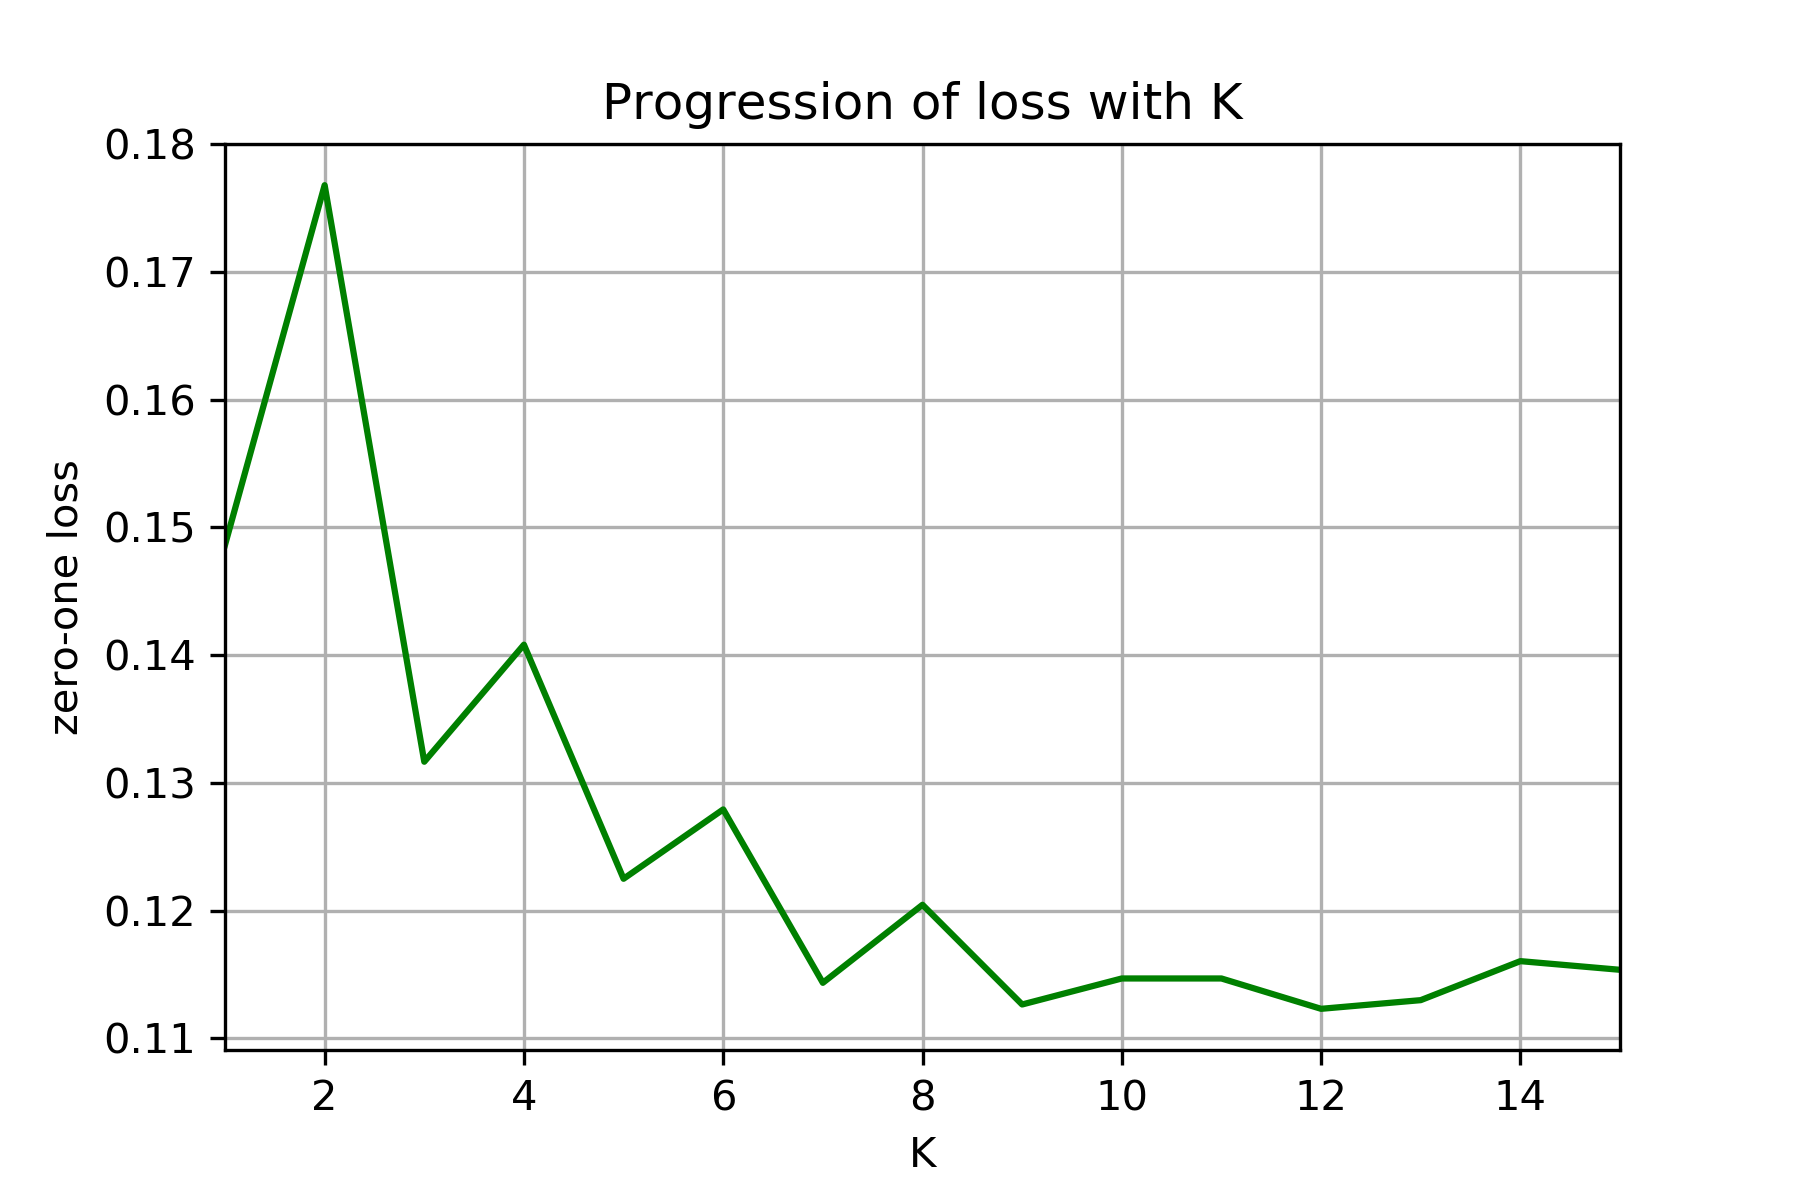
\includegraphics[width=12cm]{error_uniform_(mid_zoom)}
    \caption{Zero-one loss curve (uniform weights}
    \label{fig:ex2-b-error_uniform_1}
\end{figure}

\begin{figure}[H]
    \centering
    \includegraphics[width=12cm]{error_uniform_(full_zoom)}
    \caption{Zero-one loss curve (uniform weights}
    \label{fig:ex2-b-error_uniform_2}
\end{figure}

\begin{figure}[H]
    \centering
    \includegraphics[width=12cm]{error_distance}
    \caption{Zero-one loss curve (inversely proportional to distance weights}
    \label{fig:ex2-b-error_distance_0}
\end{figure}

\begin{figure}[H]
    \centering
    \includegraphics[width=12cm]{error_distance_(mid_zoom)}
    \caption{Zero-one loss curve (inversely proportional to distance weights}
    \label{fig:ex2-b-error_distance_1}
\end{figure}

\begin{figure}[H]
    \centering
    \includegraphics[width=12cm]{error_distance_(full_zoom)}
    \caption{Zero-one loss curve (inversely proportional to distance weights}
    \label{fig:ex2-b-error_distance_2}
\end{figure}

%=================================================
\end{document}
